\documentclass{article}
\usepackage{amsmath}
\usepackage{amsthm}
\usepackage{bm}
\usepackage{amssymb}
\usepackage{mathrsfs}
\usepackage{mathtools}
\usepackage{cancel}
\usepackage{graphicx}
\usepackage{pgfplots}
\usepackage{tikz}
\usepackage{epstopdf}
\usepackage{inputenc}
\usepackage{geometry}
\usepackage{float}
\usepackage{multirow}
\usepackage{comment}
\usepackage{listings}
\usepackage{pgfplotstable}

\usetikzlibrary{calc, patterns, angles, quotes, matrix}



\definecolor{myred}{rgb}{0.5,0,0}
\definecolor{mygreen}{rgb}{0,0.6,0}
\definecolor{mygray}{rgb}{0.5,0.5,0.5}
\definecolor{mymauve}{rgb}{0.58,0,0.82}
\definecolor{elemEXBLUE}{rgb}{0,0.44,0.73}

\definecolor{Blue}{rgb}{0, 0.06, 0.65}
\definecolor{YellowGreen}{rgb}{0.39, 0.58, 0.49}
\definecolor{ForestGreen}{rgb}{0.156, 0.49, 0.196}
\definecolor{Blue}{rgb}{0, 0.06, 0.65}

\lstdefinestyle{PythonSyntax}{
  language=Python,
  backgroundcolor=\color{white},   % choose the background color
  basicstyle=\footnotesize\ttfamily,        % size of fonts used for the code
  breaklines=true,                 % automatic line breaking only at whitespace
  captionpos=b,                    % sets the caption-position to bottom
  frame=single, 
  commentstyle=\color{mygreen},    % comment style
  showspaces=false,                % show spaces adding particular underscores
  showstringspaces=false,          % underline spaces within strings
  showtabs=false,                  % show tabs within strings adding particular underscores
  escapeinside={\%*}{*)},          % if you want to add LaTeX within your code
  keywordstyle=\color{blue},       % keyword style
  stringstyle=\color{mymauve},     % string literal style
}

\lstdefinestyle{RSyntax}{ 
  language=R,                     % the language of the code
  basicstyle=\footnotesize\ttfamily,      % the size of the fonts that are used for the code
  %numbers=left,                   % where to put the line-numbers
  %numberstyle=\tiny\color{Blue},  % the style that is used for the line-numbers
  %stepnumber=1,                   % the step between two line-numbers. If it is 1, each line
  %                                % will be numbered
  %numbersep=5pt,                  % how far the line-numbers are from the code
  backgroundcolor=\color{white},  % choose the background color. You must add \usepackage{color}
  showspaces=false,               % show spaces adding particular underscores
  showstringspaces=false,         % underline spaces within strings
  showtabs=false,                 % show tabs within strings adding particular underscores
  frame=single,                   % adds a frame around the code
  rulecolor=\color{black},        % if not set, the frame-color may be changed on line-breaks within not-black text (e.g. commens (green here))
  tabsize=2,                      % sets default tabsize to 2 spaces
  captionpos=b,                   % sets the caption-position to bottom
  breaklines=true,                % sets automatic line breaking
  breakatwhitespace=false,        % sets if automatic breaks should only happen at whitespace
  keywordstyle=\color{Blue},      % keyword style
  commentstyle=\color{YellowGreen},   % comment style
  stringstyle=\color{ForestGreen}      % string literal style
} 

\makeatletter
\long\def\ifnodedefined#1#2#3{%
    \@ifundefined{pgf@sh@ns@#1}{#3}{#2}%
}

\pgfplotsset{
    discontinuous/.style={
    scatter,
    scatter/@pre marker code/.code={
        \ifnodedefined{marker}{
            \pgfpointdiff{\pgfpointanchor{marker}{center}}%
             {\pgfpoint{0}{0}}%
             \ifdim\pgf@y>0pt
                \tikzset{options/.style={mark=*, fill=white}}
                \draw [densely dashed] (marker-|0,0) -- (0,0);
                \draw[options] plot coordinates {(marker-|0,0)};
             \else
                \tikzset{options/.style={mark=none}}
             \fi
        }{
            \tikzset{options/.style={mark=none}}        
        }
        \coordinate (marker) at (0,0);
        \begin{scope}[options, fill=blue]
    },
    scatter/@post marker code/.code={\end{scope}}
    }
}




\newcommand{\sigmah}{\hat{\sigma}}
\newcommand{\thetah}{\hat{\theta}}
\newcommand{\tspan}{\text{span}}
\newcommand{\tdim}{\text{dim}}
\newcommand{\trank}[1]{\text{rank($#1$)}}
\newcommand{\tmin}{\text{min}}
\newcommand{\tker}{\text{ker}}
\newcommand{\tim}{\text{Im}}
\newcommand{\ttr}{\text{trace}}
\newcommand{\E}{\mathbb{E}}
\newcommand{\V}{\text{Var}}
\newcommand{\R}{\mathbb{R}}
\newcommand{\N}{\mathbb{N}}
\newcommand{\mc}[1]{\mathcal{#1}}
\newcommand{\mb}[1]{\mathbf{#1}}
\newcommand{\trmt}[1]{\mb{#1}_{\Phi}}
\newcommand{\wop}[2]{\langle #1, #2\rangle} % wedge operator
\newcommand{\ssp}{\;\;\;} % space
\renewcommand{\P}{\mathbb{P}}
\newcommand{\ra}{\rightarrow}
\newcommand{\imp}{\;\;\implies\;\;}
%\newcommand{\PR}{\textsc{\textbf{Proof}}}

%ELEM
\newcommand{\EX}[1]{\medskip\noindent\textcolor{elemEXBLUE}{\textbf{Ex. #1}}}

\pgfplotsset{compat=1.16}


\begin{document}

\noindent
{\Huge \textbf{All of Statistics}}

\bigskip\noindent
My proposed solutions to the book:

\medskip\noindent
{\Large\textbf{All of Statistics}} - \textbf{A Concise Course in Statistical Inference}.%, ninth edition.

\medskip\noindent
Publishing code and pdf to the following GitHub repository.\\
\texttt{https://github.com/CoveredInChocolate/AllStatistics}

\bigskip\noindent
Let me know if you find any mistakes! I am sure there are plenty...

\tableofcontents

\newpage
\section{Probability}

\subsection*{Exercises}

%%%%%%%%%%%%%%%%%%%%%%%%%%%%%%%%%%%%%%%%%%%%%%%%%%%%%%%%%%%%%%%%%%%%%%%%%%%%%%%
\textbf{1.1}\\  % PDF page 13
Proving the Continuity of Probabilities.

\bigskip\noindent
\textbf{1.8 Theorem} (Continuity of Probabilities). If $A_n\rightarrow A$
then
\[
    \P(A_n)\rightarrow\P(A)
\]
as $n\rightarrow\infty$.

\bigskip\noindent
\textsc{Proof}. Suppose that $A_n$ is monotone increasing so that
$A_1\subset A_2 \subset\ldots$.
Let $A = \lim_{n\ra\infty} A_n = \bigcup_{i=1}^\infty A_i$.
Define:
\begin{align*}
    B_1 &= A_1 \\
    B_2 &= \{\omega\in\Omega \;:\; \omega\in A_2,\omega\not\in A_1\} \\
    B_3 &= \{\omega\in\Omega \;:\; \omega\in A_3,\omega\not\in A_2,\omega\not\in A_1\} \\
    \vdots &
\end{align*}
\textbf{(1)} Showing that $B_i$ are disjoint sets.\\
We have $B_1 = A_1$. Since $B_2 = \{\omega\in\Omega \;:\; \omega\in A_2,\omega\not\in A_1\}$,
we can rewrite this as $B_2 = A_2 - A_1$ by definition of set difference.

Since $B_3 = \{\omega\in\Omega \;:\; \omega\in A_3,\omega\not\in A_2,\omega\not\in A_1\}$
and since $A_1\subset A_2$, we can rewrite this as $B_3 = A_3 - (A_1\bigcup A_2)$.
In general; $B_k = A_k - (\bigcup_{i=1}^{k-1}A_i)$.

Assuming some random sets $B_m$, $B_p$ for some $m,p\in\N$. Without loss of generality,
we assume $m > p$. Then:
\begin{align*}
    B_m\bigcap B_p &=
    \Big(A_m - (\bigcup_{i=1}^{m-1}A_i)\Big)\bigcap \Big(A_p - (\bigcup_{i=1}^{p-1}A_i)\Big)\\
    &= 
    \Big(A_m \bigcap(\bigcup_{i=1}^{m-1}A_i)^c\Big)\bigcap \Big(A_p \bigcap (\bigcup_{i=1}^{p-1}A_i)^c\Big)\\
    \shortintertext{DeMorgan's law}
    &= 
    \Big(A_m \cap A_1^c \cap A_2^c \cap \ldots \cap A_p^c \cap \ldots \cap A_{m-1}^c\Big)\bigcap
    \Big(A_p \cap A_1^c \cap A_2^c \cap \ldots \cap A_{p-1}^c\Big) \\
\shortintertext{Reshuffling terms and repeated use of $C\cap C = C$}
    &= A_m \cap A_1^c \cap A_2^c \cap \ldots \cap \underbrace{A_p^c\cap A_p}_{=\emptyset} \cap \ldots \cap A_{m-1}^c\Big) \\
    &= \emptyset
\end{align*}
Since $B_m\cap B_p = \emptyset$, they are disjoint. (\emph{Quite certain this is a correct argument, but could have
made it a bit easier by going directly to the $A_3\cap A_2^c\cap A_1^c$ version of the sets.})


\medskip\noindent
\textbf{(2)} Showing that 
\[
A_n = \bigcup_{i=1}^n A_i = \bigcup_{i=1}^n B_i
\]
for each $n$. Showing this with an induction argument. Note that $A_1 = B_1$, and $A_2\cup A_1 = A_2$ since $A_1\subset A_2$. Note also that:
\begin{align*}
    B_2\cup B_1 &= (A_2\cap A_1^c)\cup A_1 \\
    &= (A_2\cup A_1)\cap(A_1^c\cup A_1) \\
    &= (A_2\cup A_1)\cap(\Omega) \\
    &= A_2\cup A_1 \\
    &= A_2
\end{align*}
So this is true for $n=2$. Assume that $A_k = \cup_{i=1}^k A_i = \cup_{i=1}^k B_i$ for $k\in\N$. Showing that this applies to $k+1$.
$$
\bigcup_{i=1}^{k+1} A_i = A_{k+1}\cup\Big(\bigcup_{i=1}^{k}A_i\Big) = A_{k+1}\cup A_k = A_{k+1}
$$
\begin{align*}
    \bigcup_{i=1}^{k+1} B_i &= B_{k+1}\cup\Big(\bigcup_{i=1}^{k} B_i\Big)\\
    &= B_{k+1}\cup A_k \\
    &= \Big[A_{k+1}\cap \Big(A_k^c\cap\ldots\cap A_1^c\Big)\Big]\cup A_k \\
    &= \Big[A_{k+1}\cap \Big(A_k\cup\ldots\cup A_1\Big)^c\Big]\cup A_k \\
    %\shortintertext{Since $A_j\subset A_{j+1}$.}
    &= \Big[A_{k+1}\cap A_k^c\Big]\cup A_k \\
    &= (A_{k+1}\cup A_k)\cap (A_k^c\cup A_k) \\
    &= (A_{k+1}\cup A_k)\cap\Omega \\
    &= A_{k+1}\cup A_k \\
    &= A_{k+1}
\end{align*}
Result verified by induction argument.

\medskip\noindent
\textbf{(3)} Showing that 
\[
\bigcup_{i=1}^\infty B_i = \bigcup_{i=1}^\infty A_i.
\tag{$\diamondsuit$}
\]
By definition:
$$
A = \lim_{n\ra\infty} A_n = \bigcup_{i=1}^\infty A_i.
$$
By step (2):
$$
A = \lim_{n\ra\infty} A_n = \lim_{n\ra\infty}\bigcup_{i=1}^n A_i = \lim_{n\ra\infty}\bigcup_{i=1}^n B_i = \bigcup_{i=1}^\infty B_i.
$$
Hence, $(\diamondsuit)$ is satisfied.

\newpage\noindent
%%%%%%%%%%%%%%%%%%%%%%%%%%%%%%%%%%%%%%%%%%%%%%%%%%%%%%%%%%%%%%%%%%%%%%%%%%%%%%%
\textbf{1.2}\\  % PDF page 13
Proving some well known results by using the axioms:
\begin{align*}
    \P(A) \geq 0,\;\forall A\subset\Omega \tag{A.1} \\
    \P(\Omega) = 1, \tag{A.2} \\
    \P\left(\bigcup_{i=1}^\infty A_i\right) = \sum_{i=1}^\infty \P(A_i) \tag{A.3}
\end{align*}
where $A_1, A_2,\ldots$ are disjoint in  $(A.3)$.

\medskip\noindent$\bullet$ \textbf{Claim}: $\P(\emptyset) = 0$.\\
\textsc{Proof}. Since $\Omega\cap\emptyset = \emptyset$ and the empty set is disjoint with itself, we can
make set $E_1 = \Omega$ and $E_k = \emptyset$ for all $k\geq 2$. Now assume for contradiction that $\P(\emptyset) = a > 0$
for some $a\in\R$. Then by $(A.3)$:
$$
\P\left(\bigcup_{i=1}^\infty E_i\right) \overset{A.3}{=} \sum_{i=1}^\infty \P(E_i) = \P(\Omega) + \sum_{i=2}^\infty \P(\emptyset)
= 1 + \sum_{i=2}^\infty a = \infty
$$
Now instead of using $(A.3)$ we use that the infinite set of $E_i$ becomes $\Omega$:
\begin{equation*}
    \P\left(\bigcup_{i=1}^\infty E_i\right) = \P(\Omega) \overset{A.2}{=} 1
\end{equation*}
We have reached a contradiction. This shows that $\P(\emptyset) = 0$. \qed
% they are disjoint
% and $\Omega = \Omega\cup\emptyset$, so by properties (A.2) and (A.3):
% $$
% 1 \overset{A.2}{=} \P(\Omega) = \P(\Omega\cup\emptyset)
% \overset{A.3}{=} \P(\Omega) + \P(\emptyset) \overset{A.2}{=} 1 + \P(\emptyset)
% $$
% So:
% \begin{equation*}
%     1 = 1 + \P(\emptyset) \;\;\Longrightarrow\;\; \P(\emptyset) = 0
%     \tag*{$\blacksquare$}
% \end{equation*}

\medskip\noindent$\bullet$ \textbf{Claim}: $A\cap B = \emptyset \;\Longrightarrow\; \P(A\cup B) = \P(A) + \P(B)$.\\
\textsc{Proof}. Set $E_1 = A$ and $E_2 = B$ and $E_k = \emptyset$ for all $k\geq 3$. Then:
\begin{equation*}
\P(A\cup B) = \P\left(\bigcup_{i=1}^\infty E_i\right) \overset{A.3}{=} \sum_{i=1}^\infty \P(E_i)
= \P(A) + \P(B) + \sum_{k=3}^\infty \P(\emptyset) = \P(A) + \P(B) + 0 = \P(A) + \P(B)
\tag*{\qed}
\end{equation*}

\medskip With this result, we can apply $(A.3)$ indirectly to any finite sum of disjoint sets.
All other sets are set to $\emptyset$ and then (A.3) is applied. Not giving a formal argument, but if $A,B,C$ are mutually disjoint
we can set $E_k = \emptyset$ for all $k\geq 4$.
$$
\P(A\cup B\cup C) = \P\left(\bigcup_{i=1}^\infty E_i\right) \overset{A.3}{=} \sum_{i=1}^\infty \P(E_i)
= \P(A) + \P(B) + \P(C) + 0 = \P(A) + \P(B) + \P(C)
$$


\medskip\noindent$\bullet$ \textbf{Claim}: $A\subset B \;\Longrightarrow\; \P(A) \leq \P(B)$.\\
\textsc{Proof}. Since $A\subset B$ we can split $B$ into two disjoint parts: $B = A\cup B-A$.
By axiom (A.3):
\begin{equation*}
\P(B) = \P(A\cup B-A) \overset{A.3}{=} \P(A) + \P(B-A) \overset{A.1}{\geq} \P(A)
\;\;\Longrightarrow\;\;
\P(A) \leq \P(B)
\tag*{\qed}
\end{equation*}

\medskip\noindent$\bullet$ \textbf{Claim}: $0\leq \P(A) \leq 1$.\\
\textsc{Proof}. Since $A\subset \Omega$ and by the previous proof: $\P(A) \leq \P(\Omega) = 1$
Combining this with axiom (A.1):
\begin{equation*}
0 \overset{A.1}{\leq} \P(A) \leq \P(\Omega) = 1
\;\;\Longrightarrow\;\;
0\leq \P(A) \leq 1
\tag*{\qed}
\end{equation*}

\medskip\noindent$\bullet$ \textbf{Claim}: $\P(A^c) = 1 - \P(A)$.\\
\textsc{Proof}. Since $A\cup A^c$ are disjoint, we get by finite version of (A.3):
$$
\P(A\cup A^c) = \P(A) + \P(A^c)
$$
Since $\Omega = A\cup A^c$ we also get by (A.2):
$$
\P(A\cup A^c) = \P(\Omega) = 1
$$
Putting them together:
\begin{equation*}
\P(A) + \P(A^c) = 1 \ssp\Longrightarrow\ssp 
\P(A^c) = 1 - \P(A)
\tag*{\qed}
\end{equation*}


\bigskip\noindent
%%%%%%%%%%%%%%%%%%%%%%%%%%%%%%%%%%%%%%%%%%%%%%%%%%%%%%%%%%%%%%%%%%%%%%%%%%%%%%%
\textbf{1.3}\\  % PDF page 14
$\Omega$ is a sample space and $A_1,A_2,\ldots$ are events. We define:
$$
B_n = \bigcup_{i=n}^\infty A_i,
\qquad
C_n = \bigcap_{i=n}^\infty A_i
$$
(a) \textbf{Claim}: $B_1\supset B_2\supset\ldots$\\
\textsc{Proof}. This follows directly from the definition of $B_n$. First we see that:
$$
B_1 = \bigcup_{i=1}^\infty A_i =
A_1 \cup \left(\bigcup_{i=2}^\infty A_i\right) \supset
\bigcup_{i=2}^\infty A_i = B_2, \;\;\Longrightarrow\;\;
B_1\supset B_2
$$
The same argument can be used for some $k\in\N$.
$$
B_k = \bigcup_{i=k}^\infty A_i =
A_{k} \cup \left(\bigcup_{i=k+1}^\infty A_i\right) \supset
\bigcup_{i=k+1}^\infty A_i = B_{k+1}, \;\;\Longrightarrow\;\;
B_{k}\supset B_{k+1}
$$
From this, it follows that $B_1\supset B_2 \supset \ldots$. \qed

\medskip\noindent
\textbf{Claim}: $C_1\subset C_2\subset\ldots$\\
\textsc{Proof}. This also follows directly from the definition. First note that:
$$
C_1 = \bigcap_{i=1}^\infty A_i = A_1\cap\left(\bigcap_{i=2}^\infty A_i\right) \subset
\bigcap_{i=2}^\infty A_i = C_2 \;\;\Longrightarrow\;\;
C_1\subset C_2
$$
And, in general, for some $k\in\N$.
$$
C_k = \bigcap_{i=k}^\infty A_i = A_k\cap\left(\bigcap_{i=k+1}^\infty A_i\right) \subset
\bigcap_{i=k+1}^\infty A_i = C_{k+1} \;\;\Longrightarrow\;\;
C_k\subset C_{k+1}
$$
This shows that $C_1\subset C_2\subset\ldots$. \qed

\newpage\noindent
(b) \textbf{Claim}:
$$
\omega\in \bigcap_{n=1}^\infty B_n
\;\;\Longleftrightarrow\;\;
\omega\in A_1,A_2,\ldots
$$
\textsc{Proof}.\\
$\Rightarrow$) Assume $\omega\in \bigcap_{n=1}^\infty B_n$, which means $\omega\in B_k,\forall k\in\N$. Expanding the intersection:
$$
\omega\in B_1\cap B_2\cap\ldots\cap B_k\cap B_{k+1}\cap\ldots
$$
Now, from the definition of $B_1$, like we used above:
$$
B_1 = \bigcup_{i=1}^\infty A_i = A_1\cup \bigcup_{i=2}^\infty A_i = A_1\cup B_2
$$
So, we can write: $B_1\cap B_2 = (A_1\cup B_2)\cap B_2 = (A_1\cap B_2)\cup(B_2\cap B_2) = (A_1\cap B_2)\cup B_2$.
And in general:
$$
B_k = \bigcup_{i=k}^\infty A_i = A_k\cup \bigcup_{i=k+1}^\infty A_i = A_k\cup B_{k+1},
$$
so $B_k\cap B_{k+1} = (A_k\cup B_{k+1})\cap B_{k+1} = (A_k\cap B_{k+1})\cup B_{k+1}$. So, each $B_i$ can be
decomposed into $(A_i\cap B_{i+1})\cup B_{i+1}$ and the $B_{i+1}$ is rewritten as its own intersection.
Ultimately, we get:
\begin{align*}
    &\omega\in B_1\cap B_2\cap B_3\cap\ldots\cap B_k\cap B_{k+1}\cap\ldots \;\;\Longrightarrow \\
    &\omega\in \big[(A_1\cap B_2)\cup B_2\big]\cap B_3\cap\ldots\cap B_k\cap B_{k+1}\cap\ldots  \;\;\Longrightarrow \\
    &\omega\in \big[(A_1\cap B_2)\cup (A_2\cap B_3)\cup B_3\big]\cap\ldots\cap B_k\cap B_{k+1}\cap\ldots  \;\;\Longrightarrow \\
    &\omega\in (A_1\cap B_2)\cup (A_2\cap B_3)\cup\ldots \cup(A_k\cap B_{k+1})\cup(A_{k+1}\cap B_{k+2})\cup\ldots\;\;\Longrightarrow \\
    &\omega\in (A_k\cap B_{k+1})\forall k\in\N \;\;\text{by assumption that}\; \omega\in B_k\forall k\in\N \;\;\Longrightarrow \\
    &\omega\in A_k,\forall k\in\N
\end{align*}
which means $\omega\in A_1,A_2,\ldots,A_k,A_{k+1},\ldots$ proving the first implication.

\medskip\noindent $\Leftarrow$) Now assume $\omega\in A_1,A_2,\ldots, A_k,\ldots$ which means
that $\omega\in A_k$ for any $k\in\N$. Then,
$$
\omega\in A_k \;\Longrightarrow\; \omega\in A_k\cup\left(\bigcup_{i=k+1}^\infty A_i\right)
= \bigcup_{i=k}^\infty A_i = B_k
\;\;\Longrightarrow\;\;
\omega\in B_k,
$$
So $\omega$ is included in all $B_k$ for $k\in\N$ which means $\omega$ is also in the intersection of all $B_i$.
\[
\omega\in B_1,B_2,\ldots, B_k,\ldots \;\;\Longrightarrow\;\;
\omega\in \bigcap_{n=1}^\infty B_n
\]
By implication both ways, we have proved the equivalency.\qed\\

\bigskip\noindent
(c) \emph{Skipped}.


\newpage\noindent
%%%%%%%%%%%%%%%%%%%%%%%%%%%%%%%%%%%%%%%%%%%%%%%%%%%%%%%%%%%%%%%%%%%%%%%%%%%%%%%
\textbf{1.4}\\  % PDF page 14
Proving DeMorgan's laws. First in the case when $i = \{1,2,\ldots, n\}$.

\medskip\noindent
\textbf{Claim}:
$$
\left(\bigcup_{i=1}^n A_i\right)^c = \bigcap_{i=1}^nA_i^c
$$
\textsc{Proof}. Starting with $x\in(\cup_{i=1}^n A_i)^c$, we have the following equivalencies:
\begin{align*}
    x\in \left(\bigcup_{i=1}^n A_i\right)^c
    &\;\;\Longleftrightarrow\;\;
    x\not\in \bigcup_{i=1}^n A_i \\
    &\;\;\Longleftrightarrow\;\;
    x\not\in A_1\;\text{and}\; x\not\in A_2\;\text{and}\;\ldots\;\text{and}\; x\not\in A_n \\
    &\;\;\Longleftrightarrow\;\;
    x\in A_1^c\;\text{and}\; x\in A_2^c\;\text{and}\;\ldots\;\text{and}\; x\in A_n^c \\
    &\;\;\Longleftrightarrow\;\;
    x\in \bigcap_{i=1}^nA_i^c
    \tag*{\qed}
\end{align*}
\textbf{Claim}:
$$
\left(\bigcap_{i=1}^n A_i\right)^c = \bigcup_{i=1}^nA_i^c
$$
\textsc{Proof}. Starting with $x\in(\cap_{i=1}^n A_i)^c$, we have the following equivalencies:
\begin{align*}
    x\in \left(\bigcap_{i=1}^n A_i\right)^c
    &\;\;\Longleftrightarrow\;\;
    x\not\in \bigcap_{i=1}^n A_i \\
    &\;\;\Longleftrightarrow\;\;
    \exists p\in \{1,\ldots, n\}\;x\not\in A_p \\
    &\;\;\Longleftrightarrow\;\;
    \exists p\in \{1,\ldots, n\}\;x\in A_p^c \\
    &\;\;\Longleftrightarrow\;\;
    x\in \bigcup_{i=1}^nA_i^c
    \tag*{\qed}
\end{align*}
Proving these results for a random index set is essentially the same, except finding some way of numerating the index
set with $i_1, \ldots, i_n$ (since it has to be countably infinite) which I won't bother doing.


\bigskip\noindent
%%%%%%%%%%%%%%%%%%%%%%%%%%%%%%%%%%%%%%%%%%%%%%%%%%%%%%%%%%%%%%%%%%%%%%%%%%%%%%%
\textbf{1.5}\\  % PDF page 14
Tossing a fair coin until we get exactly two heads. Description of the sample space:
$$
\Omega = \{(\omega_1, \omega_2, \ldots, \omega_{k-1},\omega_k) :
\omega_i\in\{H, T\}, \omega_{k-1} = \omega_k = H, \omega_{p-1} = H \,\Rightarrow\,\omega_p = T, p<k \}
$$
Now, to calculate the probability that there will be exactly $k$ tosses. Let us look at a few specific examples:
\begin{align*}
    &k=2: \{H, H\} \;\;\Longrightarrow \P(2) = \frac{1}{2^2} = \frac{1}{4} = 0.25\\
    &k=3: \{T, H, H\} \;\;\Longrightarrow \P(3) = \frac{1}{2^3} = \frac{1}{8} = 0.125
\end{align*}
For all tosses after $k> 3$, the last three tosses have to be $\{T,H,H\}$.

\newpage\noindent
\begin{align*}
    &k=4:\;\;
    \left.
    \begin{matrix} 
        H \\ 
        T \\ 
    \end{matrix}
    \right|,T, H, H
    = 2\cdot \frac{1}{2^4} = \frac{1}{8} = 0.125\\
    &k=5:\;\;
    \left.
    \begin{matrix} 
        TT \\ 
        TH \\ 
        HT \\ 
    \end{matrix}
    \right|,T, H, H
    = 3\cdot \frac{1}{2^5} = \frac{3}{32} = 0.09375\\
    &k=6:\;\;
    \left.
    \begin{matrix} 
        TTT \\ 
        TTH \\ 
        THT \\ 
        HTT \\ 
        HTH \\ 
    \end{matrix}
    \right|,T, H, H
    = 5\cdot \frac{1}{2^6} = \frac{5}{64} = 0.078125 \\
    &k=7\;\;
    \left.
    \begin{matrix} 
        TTTT \\ 
        TTTH \\ 
        TTHT \\ 
        THTT \\ 
        HTTT \\ 
        THTH \\ 
        HTHT \\ 
        HTTH \\ 
    \end{matrix}
    \right|,T, H, H
    = 8\cdot \frac{1}{2^7} = \frac{1}{2^4} = \frac{1}{16} = 0.0625
\end{align*}
We can see a pattern emerging. The last three tosses are fixed, and for the first $k-3$ tosses, we have to count
all the combinations that do not contain 2 simultaneous H. The details are quite interesting, and it turns out
that the number after the $k-3$ first tosses follows the Fibonacci sequence (as we can see above). Defining:
$$
F(1) = 2, F(2) = 3, F(3) = 5, \ldots
$$
In general, we will then get:
$$
\P(K=k) =
\left\{
    \begin{matrix}
        \displaystyle\frac{1}{2^k} & k = 2,3 \\
        \rule{0pt}{22pt}\displaystyle\frac{F(k-3)}{2^k} & k > 3
    \end{matrix}
\right.
$$

\bigskip\noindent
%%%%%%%%%%%%%%%%%%%%%%%%%%%%%%%%%%%%%%%%%%%%%%%%%%%%%%%%%%%%%%%%%%%%%%%%%%%%%%%
\textbf{1.6}\\  % PDF page 14
Let the sample space be $\Omega = \{0, 1, 2, \ldots\}$ (which is $\{0\}\cup\N$). We are going to prove that there
is no uniform distribution on this sample space. That is, if $\P(A) = \P(B)$ whenver $|A| = |B|$ (the cardinality of the sets)
then $\P$ cannot satisfy the axioms of probability. 

The first two properties are satisfied. If we take some $k\in\N$ and define $A_1 = \{1, \ldots, k\}$ in such a way that
$P(A_1) > 0$, and generally define $A_m = \{mk+1, mk+2, \ldots, mk + k\}$, then $A_n\cap A_m = \emptyset$. (This can be
checked by setting $k=100$ and $n=5$ and $m=6$ for instance). Also, $|A_n| = |A_m|$ and $\P(A_n) = \P(A_m) > 0$.
This will cause problems in the third axiom:
$$
\P\left(\bigcup_{i=1}^\infty A_i\right) = \sum_{i=1}^\infty \P(A_i) = \infty,
$$
since we are summing an infinite number of positive values. The axioms of probability are not satisfied, so we cannot
have a uniform distribution on $\{0, 1, 2, \ldots\}$.

\bigskip\noindent
%%%%%%%%%%%%%%%%%%%%%%%%%%%%%%%%%%%%%%%%%%%%%%%%%%%%%%%%%%%%%%%%%%%%%%%%%%%%%%%
\textbf{1.7}\\  % PDF page 14
For some events $A_1, A_2, \ldots$, we are going to show that:
$$
\P\left(\bigcup_{n=1}^\infty A_n\right) \leq \sum_{n=1}^\infty \P(A_n).
$$
\textsc{Proof}. Following the hint, we define:
$$
B_n = A_n - \bigcup_{i=1}^{n-1} A_i.
$$
Next, we show that any $B_m$ and $B_n$ are disjoint for $n,m\in\N$ and $m>n$.
\begin{align*}
    B_m\cap B_n &= \left(A_m - \bigcup_{i=1}^{m-1} A_i\right)\cap\left(A_n - \bigcup_{i=1}^{n-1} A_i\right) \\
    &= \left(A_m \cap\left(\bigcup_{i=1}^{m-1} A_i\right)^c\right)\cap\left(A_n \cap\left(\bigcup_{i=1}^{n-1} A_i\right)^c\right) \\
    &= \left(A_m \cap\bigcap_{i=1}^{m-1} A_i^c\right)\cap\left(A_n \cap\bigcap_{i=1}^{n-1} A_i^c\right) \\
    &= \Big(A_m\cap A_{m-1}^c\cap\ldots\cap A_n^c\cap\ldots\cap A_2^c\cap A_1^c\Big)\cap\Big(A_n\cap A_{n-1}^c\cap\ldots\cap A_2^c\cap A_1^c\Big)  \\
    &= A_m\cap A_{m-1}^c\cap\ldots\cap A_2^c\cap A_1^c\cap A_{n-1}^c\cap\ldots\cap A_2^c\cap A_1^c\cap 
    \underbrace{A_n^c\cap A_n}_{=\emptyset} \\
    &= \emptyset
\end{align*}
Hence, the sets $B_i$ are mutually disjoint. Next, we show that:
$$
\left(\bigcup_{n=1}^\infty A_n\right) = \left(\bigcup_{n=1}^\infty B_n\right).
$$
We will use an induction argument. For the first element we have: $B_1 = A_1$, and:
\begin{align*}
    \cup_{i=1}^2 B_i &= B_1\cup B_2 \\
    &= A_1\cup (A_2 - A_1) \\
    &= A_1\cup(A_2\cap A_1^c) \\
    &= (A_1\cup A_2)\cap(A_1\cup A_1^c) \\
    &= (A_1\cup A_2)\cap\Omega \\
    &= (A_1\cup A_2) \\
    &= \cup_{i=1}^2 A_i
\end{align*}
So, we assume that for $k\in\N$, we have:
$$
\left(\bigcup_{n=1}^k A_n\right) = \left(\bigcup_{n=1}^k B_n\right),
$$
and show that this applies to $k+1$.

\newpage\noindent
\begin{align*}
    \bigcup_{i=1}^{k+1} B_i &= B_{k+1}\cup \left(\bigcup_{i=1}^{k} B_i\right) \\
    &= B_{k+1}\cup \left(\bigcup_{i=1}^{k} A_i\right) \\
    &= \left(A_{k+1} - \bigcup_{i=1}^{k} A_i\right)\cup \left(\bigcup_{i=1}^{k} A_i\right) \\
    &= \left(A_{k+1} \cap \left(\bigcup_{i=1}^{k} A_i\right)^c\right)\cup \left(\bigcup_{i=1}^{k} A_i\right) \\
    &= \left(A_{k+1} \cup \bigcup_{i=1}^{k} A_i\right)\cap \left[\left(\bigcup_{i=1}^{k} A_i\right)^c\cup\left(\bigcup_{i=1}^{k} A_i\right)\right] \\
    &= \left(\bigcup_{i=1}^{k+1} A_i\right)\cap \Omega \\
    &= \bigcup_{i=1}^{k+1} A_i
\end{align*}
So, by induction, we have verfied the equality for $k+1$, so it follows that the sets are equal for all indexes.

By definition of $B_n$, we have $B_n\subset A_n$ which means $\P(B_n)\leq \P(A_n)$. Using this, we can prove the
main statement:
\begin{equation*}
    \P\left(\bigcup_{n=1}^\infty A_n\right) = \P\left(\bigcup_{n=1}^\infty B_n\right) = \sum_{n=1}^\infty \P(B_n) \leq \sum_{n=1}^\infty \P(A_n).
    \tag*{\qed}
\end{equation*}

\bigskip\noindent
%%%%%%%%%%%%%%%%%%%%%%%%%%%%%%%%%%%%%%%%%%%%%%%%%%%%%%%%%%%%%%%%%%%%%%%%%%%%%%%
\textbf{1.8}\\  % PDF page 14
Suppose that $\P(A_i) = 1$ for each $A_i$. We are going to prove that:
$$
\P\left(\bigcap_{i=1}^\infty A_i\right) = 1.
$$
\textsc{Proof}. We will prove this by induction. For events $A_1$ and $A_2$,
we know that $\P(A_1) = 1$ and $\P(A_2) = 1$. 
By the probability axioms:
$$
A_1\subset A_1\cup A_2 \subset \Omega \;\;\implies\;\;  \P(A_1) \leq \P(A_1\cup A_2) \leq \P(\Omega)
$$
Using that $\P(A_1) = 1$ and $\P(\Omega) = 1$:
$$
1 \leq \P(A_1\cup A_2) \leq 1 \;\;\implies\;\;  \P(A_1\cup A_2) = 1
$$
By Lemma 1.6:
\begin{align*}
    \P(A_1\cup A_2) &= \P(A_1) + \P(A_2) - \P(A_1\cap A_2) \\
    1 &= 2 -  \P(A_1\cap A_2) \\
    \P(A_1\cap A_2) &= 1
\end{align*}

\newpage\noindent
Assuming this holds for $k\in\N$, i.e.:
$$
\P\left(\bigcap_{i=1}^k A_i\right) = 1.
$$
To simplify the notation, we call this intersection $W_k$, so $\P(W_k) = 1$.
Now we will show it also applies to $k+1$. 
$$
A_1\cap A_2\cap\ldots\cap A_k\cap A_{k+1} = W_k\cap A_{k+1}
$$
Again, from the probability axioms:
$$
W_k\subset W_k\cup A_{k+1} \subset \Omega \;\;\implies\;\;  \P(W_k) \leq \P(W_k\cup A_{k+1}) \leq \P(\Omega)
$$
Using that $\P(W_k) = 1$ and $\P(\Omega) = 1$:
$$
1 \leq \P(W_k\cup A_{k+1}) \leq 1 \;\;\implies\;\;  \P(W_k\cup A_{k+1}) = 1
$$
By Lemma 1.6, and using that $\P(A_i) = 1$ for each $i$:
\begin{align*}
    \P(W_k\cup A_{k+1}) &= \P(W_k) + \P(A_{k+1}) - \P(W_k\cap A_{k+1}) \\
    1 &= 2 -  \P(W_k\cap A_{k+1}) \\
    \P(W_k\cap A_{k+1}) &= 1 \\
    \P\left(\bigcap_{i=1}^k A_i\cap A_{k+1}\right) &= 1\\
    \P\left(\bigcap_{i=1}^{k+1} A_i\right) &= 1
\end{align*}
Which verifies that equality holds for $k+1$. By induction, we can conclude that:
\begin{equation*}
    \P\left(\bigcap_{i=1}^\infty A_i\right) = 1.
    \tag*{\qed}
\end{equation*}

\bigskip\noindent
%%%%%%%%%%%%%%%%%%%%%%%%%%%%%%%%%%%%%%%%%%%%%%%%%%%%%%%%%%%%%%%%%%%%%%%%%%%%%%%
\textbf{1.9}\\  % PDF page 14
For a fixed $B$ such that $\P(B) > 0$, we will show that $\P(\cdot|B)$ satisfies
the axioms of probability. Recalling the definition of conditional probability:
$$
\P(A|B) = \frac{\P(A\cap B)}{\P(B)}
$$
$\bullet$ \textbf{Axiom 1}. $\P(A|B)\geq 0$ for all $A$.\\
\textsc{Proof}. The set $A\cap B$ is an event wrt. $\P(\cdot)$, so $\P(A\cap B) = a \geq 0$.
$$
\P(A|B) = \frac{\P(A\cap B)}{\P(B)} = \frac{a}{\P(B)} \geq 0,
$$
since $\P(B) > 0$. \qed

\newpage\noindent
$\bullet$ \textbf{Axiom 2}. $\P(\Omega|B) = 1$.\\
\textsc{Proof}. 
\begin{equation*}
    \P(\Omega|B) = \frac{\P(\Omega\cap B)}{\P(B)} = \frac{\P(B)}{\P(B)} = 1
    \tag*{\qed}
\end{equation*}

\bigskip\noindent
$\bullet$ \textbf{Axiom 3}. If $A_1, A_2, \ldots$ are disjoint, then:
$$
\P\left(\bigcup_{i=1}^\infty A_i\Big| B\right) =
\sum_{i=1}^\infty \P(A_i|B)
$$
\textsc{Proof}. First a supporting argument. If we define $C_i := A_i\cap B$ for each $i$,
then $C_1, C_2, \ldots$ are mutually disjoint sets and by (A.3):
$$
\P\left(\bigcup_{i=1}^\infty C_i\right) =
\sum_{i=1}^\infty \P(C_i).
$$
This means:
$$
\P\left(\bigcup_{i=1}^\infty A_i\Big| B\right) =
\frac{\P\left(\bigcup_{i=1}^\infty A_i\cap B\right)}{\P(B)} =
\frac{\P\left(\bigcup_{i=1}^\infty C_i\right)}{\P(B)} =
\frac{\sum_{i=1}^\infty \P(C_i)}{\P(B)} =
\sum_{i=1}^\infty\frac{ \P(A_i\cap B)}{\P(B)}  =
\sum_{i=1}^\infty \P(A_i|B)
$$
which proves the final axiom for the conditional probability.\qed 

\bigskip\noindent
%%%%%%%%%%%%%%%%%%%%%%%%%%%%%%%%%%%%%%%%%%%%%%%%%%%%%%%%%%%%%%%%%%%%%%%%%%%%%%%
\textbf{1.10} Monty Hall\\  % PDF page 14
%We define the sample space. To simplify the calculations, we assume we pick door 1:
%$$
%\Omega = \{(\text{II}, \text{III}) : \omega_i\in\{1, 2, 3\}\}.
%\Omega = \{(\omega_1, \omega_2, \omega_3) : \omega_i\in\{1, 2, 3\}\}.
%$$
%where II is the door with the prize, and III is the door Monty opens.
%where $w_3$ is the selected door, $\omega_1$ is the prize and $\omega_2$ is the door
%Monty opens.
There are three doors, 1, 2, 3, and there is a prize between one of them. We don't know which
door contains the prize, so the probability of selecting the correct door is evenly spread out:
$$
P(1) = \frac{1}{3},\quad
P(2) = \frac{1}{3},\quad
P(3) = \frac{1}{3}
$$
To simplify the calculations, we assume we pick door 1, and that the prize is not behind door 3.
Now we will decide if it's better to switch or not. What is the probability that the host will
open door III conditioned on where the prize is?
\begin{align*}
    P(\text{III}|1) &= \frac{1}{2} \quad\text{(Correct door is selected, door 3 is opened randomly)} \\
    P(\text{III}|2) &= 1 \quad\;\text{(Host never reveals the prize)}\\
    P(\text{III}|3) &= 0 \quad\;\text{(Host never reveals the prize)}
\end{align*}
Now, what is the probability that the prize is behind door number 2, given that door III was opened?
This can be calculated by Bayes Law.
$$
P(A_k|B) = \frac{P(B|A_k)P(A_k)}{\sum_{i=1}^n P(B|A_i)P(A_i)}
$$

\newpage\noindent
In our case, probability of door 2 containing the prize, given that door III was opened:
\begin{align*}
    P(2|\text{III}) &=
    \frac{\P(\text{III}|2)\P(2)}{\P(\text{III}|1)\P(1) + \P(\text{III}|2)\P(2) + \P(\text{III}|3)\P(3)} \\
    &= \frac{(1)(\frac{1}{3})}{(\frac{1}{2})(\frac{1}{3}) + (1)(\frac{1}{3}) + (0)(\frac{1}{3})} \\
    &= \frac{\frac{1}{3}}{\frac{1}{6} + \frac{1}{3} + 0} = \frac{1}{3} / \frac{1}{2} \\
    &= \frac{2}{3}
\end{align*}
Probability that door 1 contains the prize, given that door III was opened:
\begin{align*}
P(1|\text{III}) &=
\frac{\P(\text{III}|1)\P(1)}{\P(\text{III}|1)\P(1) + \P(\text{III}|2)\P(2) + \P(\text{III}|3)\P(3)} \\
&= \frac{(\frac{1}{2})(\frac{1}{3})}{(\frac{1}{2})(\frac{1}{3}) + (1)(\frac{1}{3}) + (0)(\frac{1}{3})} \\
&= \frac{\frac{1}{6}}{\frac{1}{6} + \frac{1}{3} + 0} = \frac{1}{6} / \frac{1}{2} \\
&= \frac{1}{3}
\end{align*}
This shows that we are better off switching doors then remaining in the one we initially selected.

\bigskip\noindent
%%%%%%%%%%%%%%%%%%%%%%%%%%%%%%%%%%%%%%%%%%%%%%%%%%%%%%%%%%%%%%%%%%%%%%%%%%%%%%%
\textbf{1.11}\\  % PDF page 15
\textbf{Claim}. If $A$ and $B$ are independent, then $A^c$ and $B^c$ are independent.

\medskip\noindent\textsc{Proof}. By definition of independence $\P(A\cap B) = \P(A)\P(B)$.
By property of probabilities: $\P(A^c) = 1 - \P(A)$ and $\P(B^c) = 1 - \P(B)$.
Applying Lemma 1.6 to $A^c\cup B^c$:
\begin{align*}
    \P(A^c\cup B^c) &= \P(A^c) + \P(B^c) - \P(A^c\cap B^c)
    \tag{2.11.1}
    % &= \P(\Omega\cap A^c\cap\Omega\cap B^c)
\end{align*}
By property of complements, and using DeMorgan's law:
$$
\P(A\cap B) = 1 - \P([A\cap B]^c) = 1 - \P(A^c\cup B^c)
$$
Which we can rewrite in the following way, and then apply the independence of $A$ and $B$:
$$
\P(A^c\cup B^c) = 1 - \P(A\cap B) = 1 - \P(A)\P(B)
$$
By property of complements, we can represent this as:
\begin{align*}
    \P(A^c\cup B^c) &= 1 - [1 - \P(A^c)][1 - \P(B^c)] \\
    &= 1 - \big[1 - \P(B^c) - \P(A^c) + \P(A^c)\P(B^c)\big] \\
    &= \P(A^c) + \P(B^c) - \P(A^c)\P(B^c)
    \tag{2.11.2}
\end{align*}
By setting (2.11.1) equal to (2.11.2) we can deduce that $\P(A^c)\P(B^c) = \P(A^c\cap B^c)$ which proves independence. \qed

\newpage\noindent
\emph{Alternative Proof}. Slightly more compact argument, but it still relies on Lemma 1.6.
\begin{align*}
    \P(A^c)\P(B^c) &\;\,= \big[1 - \P(A)\big]\big[1 - \P(B)\big] \\
    &\;\,= 1 - \P(A) - \P(B) + \P(A)\P(B) \\
    &\;\,= 1 - \big[\P(A) + \P(B) - \P(A)\P(B)\big] \\
    &\overset{IND}{=} 1 - \big[\P(A) + \P(B) - \P(A\cap B)\big] \\
    &\,\overset{L1.6}{=} 1 - \P(A\cup B) \\
    &\;\;= \P([A\cup B]^c) \\
    &\;\;= \P(A^c\cap B^c) \tag*{\qed}
\end{align*}

\bigskip\noindent
%%%%%%%%%%%%%%%%%%%%%%%%%%%%%%%%%%%%%%%%%%%%%%%%%%%%%%%%%%%%%%%%%%%%%%%%%%%%%%%
\textbf{1.12}\\  % PDF page 15
Initially, we have three cards that we call $G$ (Green both sides), $R$
(Red both sides) and $M$ (mixed colors). Next we define $r$ as 'Red side'
and $g$ as 'Green side'. We can define the joint distribution as follows:
$$
\begin{tabular}{c|ccc|c}
    & $G$ & $M$ & $R$ & \\
    \hline
    $r$ & & 1/6 & 2/6 & 1/2\\
    $g$ & 2/6 & 1/6 & & 1/2\\
    \hline
    & 1/3 & 1/3 & 1/3
\end{tabular}
$$
From the marginal distributions, we can see that the initial probabilities for selecting each card is:
$$
\P(G) = \frac{1}{3},\quad
\P(R) = \frac{1}{3},\quad
\P(M) = \frac{1}{3}
$$
And the probabilities for randomly viewing a colored card side:
$$
\P(g) = \frac{1}{2},\quad
\P(r) = \frac{1}{2}
$$
Note that we do not have independene, since $\P(G\cap g) = 2/6$ while $\P(G)\P(g) = (1/3)(1/2) = 1/6$.

We want to find the probability that we have a green card given that we observe a green side.
This can be calculated by:
$$
\P(G|g) = \frac{\P(G\cap g)}{\P(g)} = \frac{2/6}{1/2} = 4/6 = 2/3
$$
% Given that we select a card and see that it is green on one side, '$g$', what are the probabilities
% for each card? Since there are a total of 6 sides we can select:
% \begin{align*}
%     P(g|G) &= \frac{2}{6} \\ 
%     P(g|R) &= 0 \\
%     P(g|M) &= \frac{1}{6} 
% \end{align*}
% It doesn't really matter what happens when we turn the card around, all that matters is what card
% we have in our hand, so we only have to consider the conditional probabilities directly. Since
% the event $g$ has probability $3/6 = 1/2$, we can calculate the desired probabilities:
% \begin{align*}
%     \P(G\cap g) &= \P(G|g)\P(g) = \frac{2}{6}\cdot\frac{1}{2} = \frac{1}{6} \\
%     \P(R\cap g) &= \P(R|g)\P(g) = \frac{1}{6}\cdot\frac{1}{2} = \frac{1}{12}
% \end{align*}
% And now we can calculate the conditional probabilities:

\bigskip\noindent
%%%%%%%%%%%%%%%%%%%%%%%%%%%%%%%%%%%%%%%%%%%%%%%%%%%%%%%%%%%%%%%%%%%%%%%%%%%%%%%
\textbf{1.13}\\  % PDF page 15
A fair coin is thrown until we have both H and T.\\
(a) The sample space is:
$$
\Omega = \{(\omega_1, \ldots, \omega_K) : \omega_i\in\{H, T\}, 1\leq i\leq K\;\text{and}\; \omega_{K-1}\not=\omega_{K}, K \geq 2\}
$$
(b) The probability of getting 3 tosses can only happen in two ways $(H,H,T)$ and $(T,T,H)$. So:
$$
P(K = 3) = 2\cdot\frac{1}{2^3} = \frac{1}{4}
$$
(it would be more complicated if it were e.g. $K\leq 3$).


\newpage\noindent
%%%%%%%%%%%%%%%%%%%%%%%%%%%%%%%%%%%%%%%%%%%%%%%%%%%%%%%%%%%%%%%%%%%%%%%%%%%%%%%
\textbf{1.14}\\  % PDF page 15
\textbf{Claim}: If $\P(A) = 0$ or $\P(A) = 1$, then $A$ is independent of every other event.

\bigskip\noindent
\textsc{Proof}. First consider the case $\P(A) = 0$. Obviously, for any $E\in\Omega$:
$$
\P(A)\P(E) = 0\cdot\P(E) = 0.
$$
By the axioms of probability: $A\cap E\subset A$ so $\P(A\cap E) \leq \P(A) = 0$
and since for any event: $0\leq \P(A\cap E)$ we can conclude that $\P(A\cap E) = 0$.
So:
$$
\P(A\cap E) = 0 = \P(A)\P(E)
\;\;\implies\;\;
\P(A\cap E) = \P(A)\P(E)
$$
which proves independence.

Now consider $\P(A) = 1$. Then, for any event $E\in\Omega$:
$$
\P(A)\P(E) = 1\cdot\P(E) = \P(E).
$$
Since $A\subset A\cup E \subset \Omega$, then $\P(A)\leq\P(A\cup E) \leq \P(\Omega)$. We know the probabilities
of $A$ and $\Omega$, so $1\leq \P(A\cup E)\leq 1$ means that $\P(A\cup E) = 1$. By Lemma 1.6:
\begin{align*}
    \P(A\cup B) &= \P(A) + \P(E) - \P(A\cap E) \\
    1 &= 1 + \P(E) - \P(A\cap E) \\
    \P(A\cap E) &= \P(E)
\end{align*}
In conclusion:
$$
\P(A\cap E) = \P(E) = \P(A)\P(E)
\imp
\P(A\cap E) = \P(A)\P(E)
$$
which proves independence.\qed

\bigskip\bigskip\noindent
\textbf{Claim}: If $A$ is independent of itself, then $\P(A) = 0$ or $\P(A) = 1$.

\bigskip\noindent\textsc{Proof}. If $A$ is independent of itself, we can write:
\begin{align*}
    \P(A\cap A) &= \P(A)\P(A) \\
    \P(A) &= \P(A)^2
\end{align*}
since $A\cap A = A$. We can write this as an equation, by defining $p := \P(A)$.
\begin{align*}
    p &= p^2 \\
    p^2 - p &= 0 \\
    p(p - 1) &= 0
\end{align*}
This equation is solved when $p = \P(A) = 1$ or $p = \P(A) = 0$.\qed


\newpage\noindent
%%%%%%%%%%%%%%%%%%%%%%%%%%%%%%%%%%%%%%%%%%%%%%%%%%%%%%%%%%%%%%%%%%%%%%%%%%%%%%%
\textbf{1.15}\\  % PDF page 15
The probability that a child has blue eyes is 1/4, $\P(B) = 1/4$. We assume independence
in the eye color of the children.

\medskip\noindent(a) Given that one child has blue eyes, what is the probability that 2 or more
children have blue eyes? Since it's given that one child has blue eyes, we just need to find
the probability that one, or both, of the remaining children have blue eyes.
Define $B_i$: as the event that child $i$ has blue eyes, and $\neg B_i$ the event that child $i$
does NOT have blue eyes. We only need to sum up the following three probabilities:
\begin{align*}
    \P(B_1\cap B_2) &= \P(B_1)\P(B_2) = \left(\frac{1}{4}\right)\left(\frac{1}{4}\right) = \frac{1}{16} \\
    \P(B_1\cap \neg B_2) &= \P(B_1)\P(\neg B_2) = \left(\frac{1}{4}\right)\left(\frac{3}{4}\right) = \frac{3}{16}\\
    \P(\neg B_1\cap B_2) &= \P(\neg B_1)\P(B_2) = \left(\frac{3}{4}\right)\left(\frac{1}{4}\right) = \frac{3}{16}
\end{align*}
By summing these up, we find that the probability of two or more children having blue eyes is $\displaystyle\frac{7}{16}$.

\medskip\noindent(b) Which child has blue eyes is irrelevant. The probability will be the same: $\displaystyle\frac{7}{16}$.


\bigskip\noindent
%%%%%%%%%%%%%%%%%%%%%%%%%%%%%%%%%%%%%%%%%%%%%%%%%%%%%%%%%%%%%%%%%%%%%%%%%%%%%%%
\textbf{1.16}\\  % PDF page 15
Proving Lemma 1.14. If $A$ and $B$ are independent events, then $\P(A|B) = \P(A)$. Also,
for any pair of events $A$ and $B$,
$$
\P(A\cap B) = \P(A|B)\P(B) = \P(B|A)\P(A).
$$
\textsc{Proof}. Suppose $A$ and $B$ are independent. By definition of independence, $\P(A\cap B) = \P(A)\P(B)$.
By definition of conditional probability:
$$
\P(A|B) = \frac{\P(A\cap B)}{\P(B)} = \frac{\P(A)\P(B)}{\P(B)} = \P(A),
$$
which proves the first statement. Again, by definition of conditional probability:
$$
\P(A|B) = \frac{\P(A\cap B)}{\P(B)} \imp \P(A\cap B) = \P(A|B)\P(B)
$$
$$
\P(B|A) = \frac{\P(B\cap A)}{\P(A)} \imp \P(A\cap B) = \P(B|A)\P(A),
$$
since $A\cap B = B\cap A$ which proves the remaining two statements.\qed


\newpage\noindent
%%%%%%%%%%%%%%%%%%%%%%%%%%%%%%%%%%%%%%%%%%%%%%%%%%%%%%%%%%%%%%%%%%%%%%%%%%%%%%%
\textbf{1.17}\\  % PDF page 15
Show that
$$
\P(A\cap B\cap C) = \P(A|B\cap C)\P(B|C)\P(C).
$$
\textsc{Proof}. Define $E := B\cap C$, so $A\cap B\cap C = A\cap E$. By Lemma 1.14:
\begin{equation*}
    \P(A\cap B\cap C) = \P(A\cap E) = \P(A|E)\P(E) = \P(A|B\cap C)\P(B\cap C)
    \tag{2.17.1}
\end{equation*}
By Lemma 1.14 again:
$$
\P(B\cap C) = \P(B|C)\P(C),
$$
which we can replace in equation (2.17.1) and get the desired result:
\begin{equation*}
    \P(A\cap B\cap C) = \P(A|B\cap C)\P(B|C)\P(C)
    \tag*{\qed}
\end{equation*}



\bigskip\noindent
%%%%%%%%%%%%%%%%%%%%%%%%%%%%%%%%%%%%%%%%%%%%%%%%%%%%%%%%%%%%%%%%%%%%%%%%%%%%%%%
\textbf{1.18}\\  % PDF page 16
Suppose $k$ events form a partition of $\Omega$, i.e. they are disjoint and
$\bigcup_{i=1}^k A_i = \Omega$. Assume that $\P(B) > 0$. If $\P(A_1|B) < \P(A_1)$
then $\P(A_i|B) > \P(A_i)$ for some $i = 2,3,\ldots, k$.

\medskip\noindent
\textsc{Proof}. %By definition of conditional probabilities:
% $$
% \P(A_i|B) = \frac{\P(A_i\cap B)}{\P(B)}
% $$
% By the assumption and using that $\P(B) > 0$ we get:
% $$
% \P(A_1|B) < \P(A_1) \imp \frac{\P(A_1\cap B)}{\P(B)} < \P(A_1)
% %\imp \P(A_1\cap B) < \P(A_1)\P(B)
% $$
By summing over all $A_i$ with and without conditioning on $B$, we get the following two equalities:
$$
\sum_{i=1}^k \P(A_i|B) = 1,
\qquad
\sum_{i=1}^k \P(A_i) = 1
$$
We can set these equal to each other:
$$
\sum_{i=1}^k \P(A_i|B) = \sum_{i=1}^k \P(A_i) 
$$
Removing the terms for $A_1$ from the sums:
$$
\P(A_1|B) + \sum_{i=2}^k \P(A_i|B) = \P(A_1) + \sum_{i=2}^k \P(A_i) 
$$
Since $\P(A_1|B) < \P(A_1)$, then $\P(A_1) - \P(A_1|B) = a > 0$ for some $a\in\R$. By subtracting $\P(A_1|B)$ from
both sides, we can write:
$$
\sum_{i=2}^k \P(A_i|B) = \P(A_1) - \P(A_1|B) + \sum_{i=2}^k \P(A_i) 
$$
$$
\sum_{i=2}^k \P(A_i|B) = a + \sum_{i=2}^k \P(A_i) \;>\; \sum_{i=2}^k \P(A_i)
$$
So, we get:
$$
\sum_{i=2}^k \P(A_i|B) \;>\; \sum_{i=2}^k \P(A_i)
$$
which means there exists some $i\in\{2, 3, \ldots, k\}$ such that $\P(A_i|B) > \P(A_i)$. \qed



\newpage\noindent
%%%%%%%%%%%%%%%%%%%%%%%%%%%%%%%%%%%%%%%%%%%%%%%%%%%%%%%%%%%%%%%%%%%%%%%%%%%%%%%
\textbf{1.19}\\  % PDF page 16
Define $M$ as Mac users, $W$ as Windows users, and $L$ as Linux users. We have:
$$
\P(M) = 0.3,\quad
\P(W) = 0.5,\quad
\P(L) = 0.2
$$
The computers are infected with a virus, which give the following probabilities:
$$
\P(V|M) = 0.65,\quad
\P(V|W) = 0.82,\quad
\P(V|L) = 0.50
$$
A person is selected at random and we learn that her computer has the virus. What is
the probability that she is using Windows? Or, what is $\P(W|V)$? We calculate this
with Bayes Law.
\begin{align*}
    \P(W|V) &= \frac{\P(V|W)\P(W)}{\P(V|M)\P(M) + \P(V|W)\P(W) + \P(V|L)\P(L)} \\
    &= \frac{(0.82)(0.5)}{(0.65)(0.3) + (0.82)(0.5) + (0.5)(0.2)} \\
    &= 0.5815
\end{align*}

\bigskip\noindent
%%%%%%%%%%%%%%%%%%%%%%%%%%%%%%%%%%%%%%%%%%%%%%%%%%%%%%%%%%%%%%%%%%%%%%%%%%%%%%%
\textbf{1.20}\\  % PDF page 16
We have a box containing 5 coins, $C_1,\ldots,C_5$. Each coin is selected at random, so $\P(C_i) = 1/5$ for all coins.
They have the following probabilities of
getting $H$ when flipped ($p_i = \P(H|C_i)$):
$$
p_1 = 0,\quad
p_2 = 1/4,\quad
p_3 = 1/2,\quad
p_4 = 3/4,\quad
p_5 = 1
$$
(a) We flip a coin and get a head. Calculate $\P(C_i|H)$ for all coins.
First an intermediary calculation:
\begin{align*}
    \sum_{i=1}^5 \P(H|C_i)\P(C_i) &= 
    \P(H|C_1)\P(C_1) + \P(H|C_2)\P(C_2) + \P(H|C_3)\P(C_3) + \P(H|C_4)\P(C_4) + \P(H|C_5)\P(C_5) \\
    &=
    \left(0\right)\left(\frac{1}{5}\right)
    + \left(\frac{1}{4}\right)\left(\frac{1}{5}\right)
    + \left(\frac{1}{2}\right)\left(\frac{1}{5}\right)
    + \left(\frac{3}{4}\right)\left(\frac{1}{5}\right)
    + \left(1\right)\left(\frac{1}{5}\right) \\
    &= 0 + \frac{1}{20} + \frac{2}{20} + \frac{3}{20} + \frac{4}{20} \\
    &= \frac{1}{2}
\end{align*}
Calculating the posterior for each $C_i$.
$$
\P(C_1|H) = 
\frac{\P(H|C_1)\P(C_1)}{\sum_{i=1}^5 \P(H|C_i)\P(C_i)}
= \frac{0}{\frac{1}{2}} = 0
$$
$$
\P(C_2|H) = 
\frac{\P(H|C_2)\P(C_2)}{\sum_{i=1}^5 \P(H|C_i)\P(C_i)}
= \frac{\frac{1}{20}}{\frac{1}{2}} = 1/10
$$
$$
\P(C_3|H) = 
\frac{\P(H|C_3)\P(C_3)}{\sum_{i=1}^5 \P(H|C_i)\P(C_i)}
= \frac{\frac{2}{20}}{\frac{1}{2}} = 2/10
$$
\newpage\noindent
$$
\P(C_4|H) = 
\frac{\P(H|C_4)\P(C_4)}{\sum_{i=1}^5 \P(H|C_i)\P(C_i)}
= \frac{\frac{3}{20}}{\frac{1}{2}} = 3/10
$$
$$
\P(C_5|H) = 
\frac{\P(H|C_5)\P(C_5)}{\sum_{i=1}^5 \P(H|C_i)\P(C_i)}
= \frac{\frac{4}{20}}{\frac{1}{2}} = 4/10
$$
(b) We toss the coin again. Finding the probability $\P(H_2|H_1)$ ($H_i$: getting $H$ on toss $i$).
We are still using the same random coin, so we must calculate the probability for all coins together.
% For $C_1$ we can't get $H$, so the probability $\P(H_2|H_1) = 0$.

% \medskip\noindent
% For $C_2$ we want to find $\P(H_2|H_1)$. This will be conditional on what coin we are using, but it will also
% be independent, since the coin doesn't remember the result from the last toss.

\newpage\noindent
\textbf{1.21}\\  % PDF page 16
Proportion of H vs T for $p=0.3$.
\begin{lstlisting}[style=RSyntax, title=R]
# 1.21 - Plotting proportion of H vs T
n = 1000
p = 0.3
coinTosses = sample(c("H","T"), prob = c(p, 1-p), size = n, replace = TRUE)
proportionHeads = rep(0, n)
headCount = 0
for(i in 1:n) {
    if (coinTosses[i] == "H") {
    headCount = headCount + 1
    } 
    proportionHeads[i] = headCount/i
} 

# PDF
pdf("~/ALLSTAT/ch1_2.21a.pdf")
plot(x = 1:n, y = proportionHeads, type = "l", ylim = c(0,1),
        main = paste0("Proportion heads for p=", p))
abline(h = p, col = "red", lty = "dashed")
dev.off()         
\end{lstlisting}

\medskip\noindent
\textbf{Result}\\
After some initial randomness due to few samples, we can see that the simulated results stabilizes
aroud 0.3, as expected.
\begin{figure}[H]
    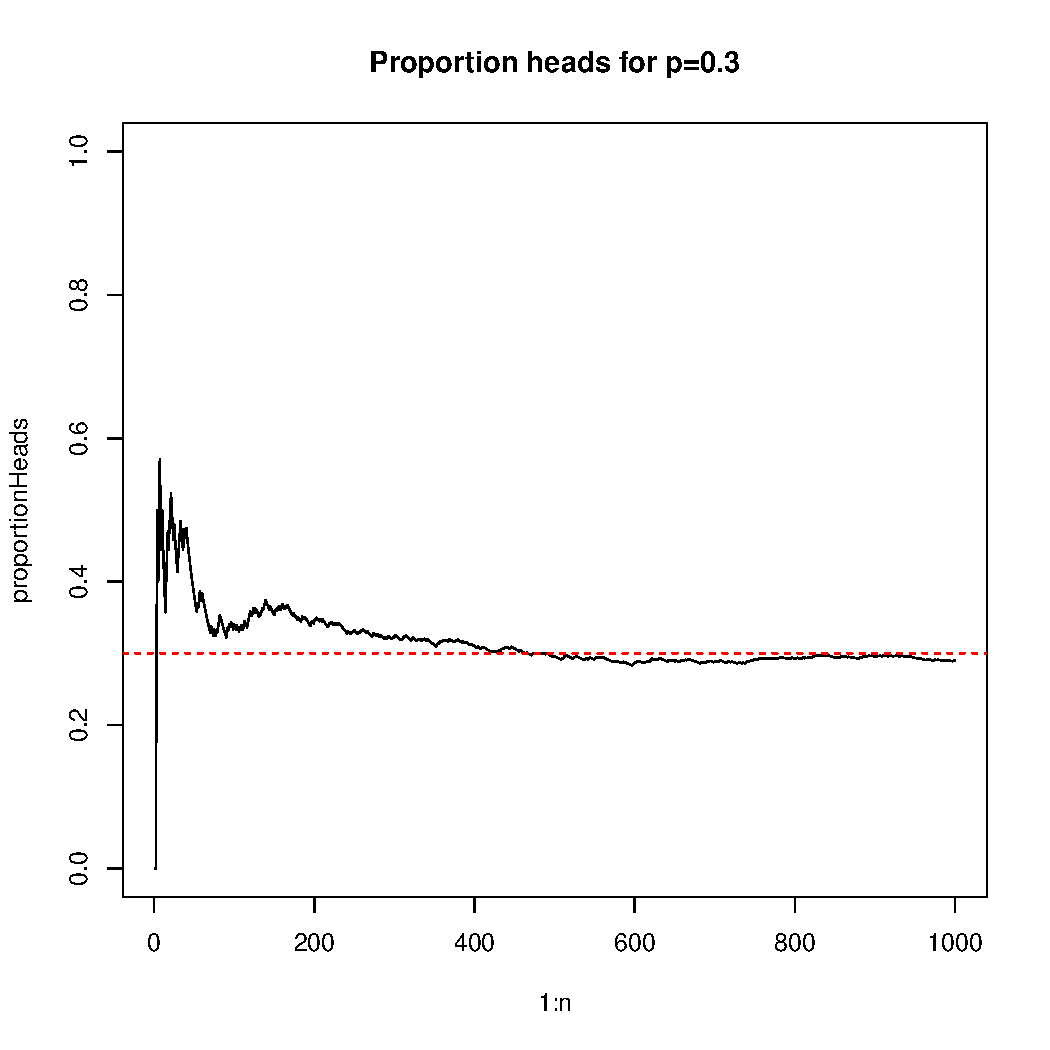
\includegraphics[width=0.6\textwidth]{ch1_2.21a.pdf}
\end{figure}


\newpage\noindent
Proportion of H vs T for $p=0.03$.
\begin{lstlisting}[style=RSyntax, title=R]
# 1.21 - Plotting proportion of H vs T
n = 5000
p = 0.03
coinTosses = sample(c("H","T"), prob = c(p, 1-p), size = n, replace = TRUE)
proportionHeads = rep(0, n)
headCount = 0
for(i in 1:n) {
    if (coinTosses[i] == "H") {
    headCount = headCount + 1
    } 
    proportionHeads[i] = headCount/i
} 

# PDF
pdf("~/ALLSTAT/ch1_2.21b.pdf")
plot(x = 1:n, y = proportionHeads, type = "l", ylim = c(0,1),
        main = paste0("Proportion heads for p=", p))
abline(h = p, col = "red", lty = "dashed")
dev.off()        
\end{lstlisting}

\medskip\noindent
\textbf{Result}\\
After some initial randomness due to few samples, we can see that the simulated results stabilizes
aroud 0.03, as expected. Did a simulation of 5000 to make the 'convergence' clearer. Note that the
y-axis only goes up to 0.1 in this plot.
\begin{figure}[H]
    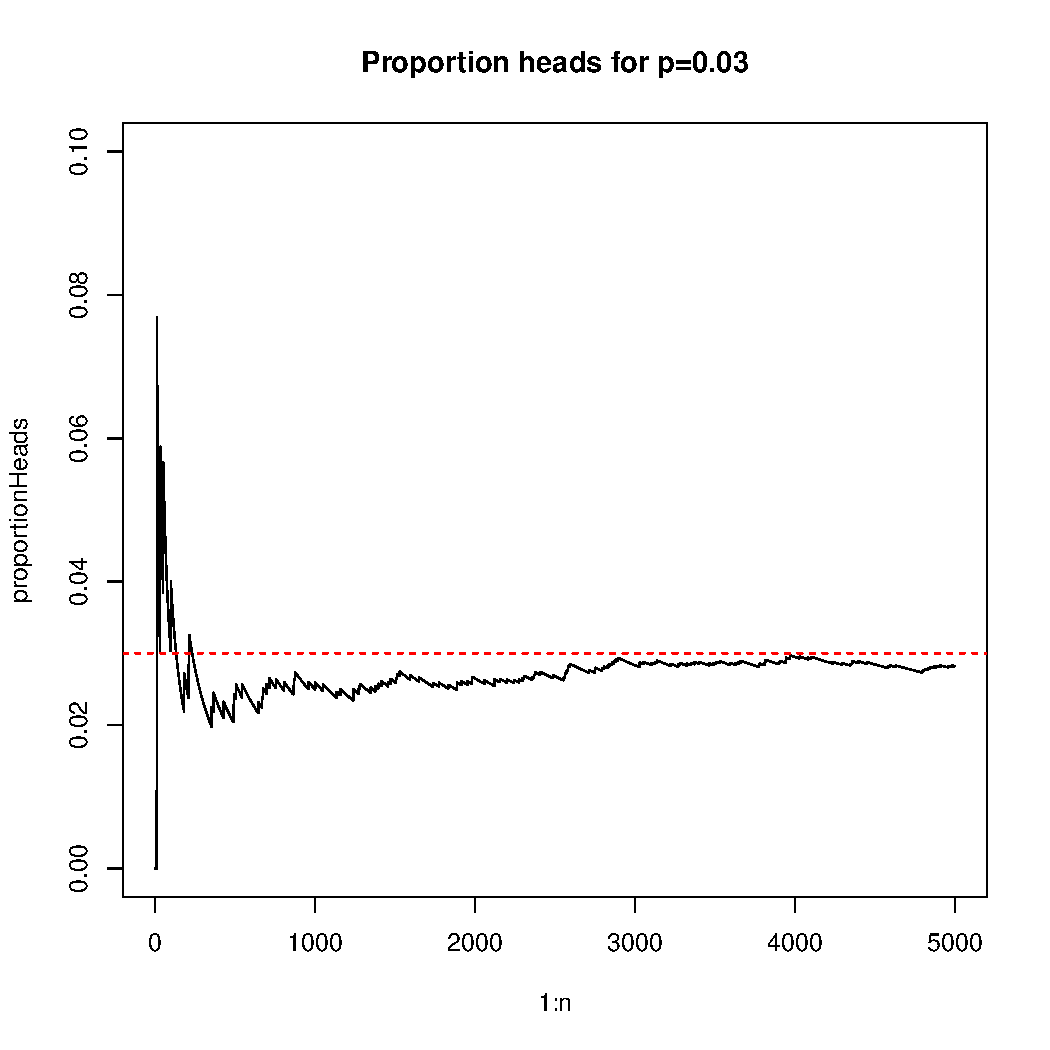
\includegraphics[width=0.6\textwidth]{ch1_2.21b.pdf}
\end{figure}



\newpage\noindent
\textbf{1.22}\\  % PDF page 16
Investigating some properties of Binomial random variables.
\begin{lstlisting}[style=RSyntax, title=R]
# 1.22 - Binomial Random Variables
REP = 10  # Number of simulations per n
p = 0.3   # Probability of H
sim10 = rep(0, REP)
sim100 = rep(0, REP)
sim1000 = rep(0, REP)
# Simulating 10
for(i in 1:REP) {
    # 1 means head
    coinTosses = sample(c(1,0), prob = c(p, 1-p), size = 10, replace = TRUE)
    sim10[i] = sum(coinTosses) 
} 
# Simulating 100
for(i in 1:REP) {
    # 1 means head
    coinTosses = sample(c(1,0), prob = c(p, 1-p), size = 100, replace = TRUE)
    sim100[i] = sum(coinTosses) 
} 
# Simulating 1000
for(i in 1:REP) {
    # 1 means head
    coinTosses = sample(c(1,0), prob = c(p, 1-p), size = 1000, replace = TRUE)
    sim1000[i] = sum(coinTosses) 
} 
df = data.frame(
    SIM10 = sim10,
    SIM100 = sim100,
    SIM1000 = sim1000
)       
# Output
df
apply(df, 2, mean)
\end{lstlisting}
As seen in the results, the mean of the 10 simulations is close to $np$ which would be 3, 30 and 300.
\begin{verbatim}
> df
    SIM10 SIM100 SIM1000
1     1     32     282
2     2     30     298
3     3     33     319
4     3     28     290
5     3     29     284
6     2     34     286
7     4     37     310
8     2     30     294
9     2     30     297
10    2     31     326
> apply(df, 2, mean)
    SIM10  SIM100 SIM1000 
    2.4    31.4   298.6 
\end{verbatim}



\newpage\noindent
\textbf{1.23}\\  % PDF page 17
Simulating conditional probabilities.
First we simulate an independent experiment.
\begin{lstlisting}[style=RSyntax, title=R]
# 1.23 - Simulating a fair die
options(digits=8)
numberOfTosses = 10000
A = c(2, 4, 6)
B = c(1, 2, 3, 4)
AandB = intersect(A, B) # c(2, 4)

dieTosses = sample(1:6, size = numberOfTosses, replace = TRUE)

# Calculating P(A), P(B), P(A)*P(B) and P(A cap B) 
PA = sum(dieTosses %in% A)/numberOfTosses
PB = sum(dieTosses %in% B)/numberOfTosses
PAandB = sum(dieTosses %in% AandB)/numberOfTosses

# Output
PA
PB
PA*PB
PAandB
\end{lstlisting}
Results from the calculation. As we can see, the estimates for $\P(A)\approx 1/2$ and
$\P(B)\approx 2/3$. Also $\P(A\cap B)\approx \P(A)\P(B) \approx 1/3$. Differences are probably due
to rounding errors.
\begin{verbatim}
> # Output
> PA
[1] 0.5005
> PB
[1] 0.6695
> PA*PB
[1] 0.33508475
> PAandB
[1] 0.3344
\end{verbatim}

\medskip\noindent
Now we will construct an experiment with a conditional probability. We will use a fair coin
and a die. When we get heads, this will correspond to 1 and the die is unchanged. If we get
tails, this will be 2 and will double the die count; so if we get tails and we roll a 2,
this will give us a 4.
$$
\begin{tabular}{c|cccccccccccc}
    \hline
    & 1 & 2 & 3 & 4 & 5 & 6 & 7 & 8 & 9 & 10 & 11 & 12 \\
    \hline
    $H$ & 1/12 & 1/12 & 1/12 & 1/12 & 1/12 & 1/12 & & & & & \\
    $T$ & & 1/12 & & 1/12& & 1/12& & 1/12& & 1/12& & 1/12 \\
    \hline
\end{tabular}
$$
Define the events: $A = \{2, 3, 4, 5, 6\}$ and $B = \{2, 4, 6, 8\}$ which will
give $A\cap B = \{2, 4, 6\}$. The theoretical probabilities are:
\begin{align*}
    \P(A) &= 8/12 = 2/3 = 0.666\\
    \P(B) &= 7/12 \approx 0.5833\\
    \P(A)\P(B) &= 7/18 \approx 0.3888\\
    \P(A\cap B) &= 1/2 = 0.5
\end{align*}


\newpage\noindent
Simulating conditional probabilities.
\begin{lstlisting}[style=RSyntax, title=R]
# 1.23 - Simulating a conditional probability
options(digits=8)
numberOfTosses = 10000
A = c(2, 3, 4, 5, 6)
B = c(2, 4, 6, 8)
AandB = intersect(A, B) # c(2, 4, 6)

dieTosses = sample(1:6, size = numberOfTosses, replace = TRUE)
coinTosses = sample(1:2, size = numberOfTosses, replace = TRUE)
jointToss = dieTosses*coinTosses

# Calculating P(A), P(B), P(A)*P(B) and P(A cap B)
PA = sum(jointToss %in% A)/numberOfTosses
PB = sum(jointToss %in% B)/numberOfTosses
PAandB = sum(jointToss %in% AandB)/numberOfTosses

# Output
PA
PB
PA*PB
PAandB    
\end{lstlisting}
\begin{verbatim}
> # Output
> PA
[1] 0.6691
> PB
[1] 0.5825
> PA*PB
[1] 0.38975075
> PAandB
[1] 0.4995
\end{verbatim}
Repeating the theoretical values from previous page:
\begin{align*}
    \P(A) &= 8/12 = 2/3 = 0.666\\
    \P(B) &= 7/12 \approx 0.5833\\
    \P(A)\P(B) &= 7/18 \approx 0.3888\\
    \P(A\cap B) &= 1/2 = 0.5
\end{align*}
The simulated results are very close to the theoretical calculations.
We can see that we do not have independence, as expected.







\begin{comment}

\bigskip\noindent
%%%%%%%%%%%%%%%%%%%%%%%%%%%%%%%%%%%%%%%%%%%%%%%%%%%%%%%%%%%%%%%%%%%%%%%%%%%%%%%
\textbf{1.X}\\  % PDF page 16


\begin{align*}
    A &= B
\end{align*}


\begin{equation*}
    A = B
    \tag*{\qed}
\end{equation*}


\end{comment}

\newpage
\section{Chapter 2 - Random Variables}

\subsection*{Exercises}

%%%%%%%%%%%%%%%%%%%%%%%%%%%%%%%%%%%%%%%%%%%%%%%%%%%%%%%%%%%%%%%%%%%%%%%%%%%%%%%
\textbf{2.1}\\  % PDF page 43
\textbf{Claim}: $\P(X = x) = F(x^+) - F(x^-)$. (Discrete)\\
\textsc{Proof}. By definition of the CDF:
$$
F(x^+) = \lim_{z\downarrow x}F(z) = \lim_{z\downarrow x}\P(X\leq z),\qquad
F(x^-) = \lim_{y\uparrow x}F(y) = \lim_{y\uparrow x}\P(X\leq y)
$$
(so $y<x$ and $y\ra x$, and $x<z$ and $x\leftarrow z$). By the right continuous property,
we can deduce that $z > y$ and we can set $z = x$ and $y = x-1$.
$$
\P(X\leq x^+) = \P(X\leq x) = \P(X = x) + \P(X \leq x-1),\quad
\P(X\leq x^-) = \P(X\leq x-1)
$$
So:
\begin{align*}
    \P(X = x) &= \P(X = x) + \P(X\leq x-1) - \P(X\leq x-1) \\
    &= \P(X\leq x) - \P(X\leq x-1) \\
    &= \P(X\leq x^+) - \P(X\leq x^-) \\
    &= F(x^+) - F(x^-)
    \tag*{\qed}
\end{align*}

\bigskip\noindent
%%%%%%%%%%%%%%%%%%%%%%%%%%%%%%%%%%%%%%%%%%%%%%%%%%%%%%%%%%%%%%%%%%%%%%%%%%%%%%%
\textbf{2.2}\\  % PDF page 44
Let $X$ be such that $\P(X = 2) = \P(X = 3) = 1/10$ and $\P(X = 5) = 8/10$.
Here is a plot of the CDF.
\begin{center}
    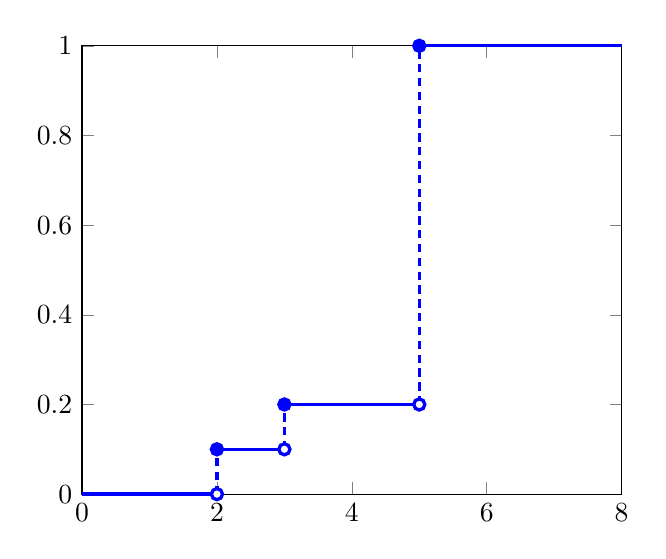
\begin{tikzpicture}
\begin{axis}[
    clip=false,
    jump mark left,
    ymin=0,ymax=1,
    xmin=0, xmax=8,
    every axis plot/.style={very thick},
    discontinuous,
    table/create on use/cumulative distribution/.style={
        create col/expr={\pgfmathaccuma + \thisrow{f(x)}}   
    }
]
\addplot [blue] table [y=cumulative distribution]{
x f(x)
0 0
2 1/10
3 1/10
5 8/10
8 0
};
\end{axis}
\end{tikzpicture}
\end{center}
By reading the plot, we can see that:
$$
\P(2 < X\leq 4.8) = F(4.8) - F(2) = 2/10 - 1/10 = 1/10
$$
$$
\P(2\leq X\leq 4.8) = F(4.8) = 2/10
$$

\bigskip\noindent
%%%%%%%%%%%%%%%%%%%%%%%%%%%%%%%%%%%%%%%%%%%%%%%%%%%%%%%%%%%%%%%%%%%%%%%%%%%%%%%
\textbf{2.3}\\  % PDF page 44
\textbf{Lemma 2.15} Let $F$ be the CDF for a random variable $X$. Then:
\begin{enumerate}
    \item $\P(X = x) = F(x) - F(x^-)$
    \item $\P(x < X\leq y) = F(y) - F(x)$
    \item $\P(X > x) = 1 - F(x)$
    \item If $X$ is continuous, then
$$
F(b) - F(a) = \P(a < X < b) = \P(a \leq X < b) = \P(a < X\leq b) = \P(a\leq X\leq b)
$$
\end{enumerate}
\textsc{Proof}. We will prove each statement in turn. (1.) was proved in exercise \textbf{2.1}.
Doing (3) first, since we need it to prove (2).

\medskip\noindent(3) By definition of complements of sets $A = \{X > x\}$ means $A^c = \{X\leq x\}$,
and it follows that:
$$
\P(X > x) = \P(A) = 1 - \P(A^c) = 1 - \P(X\leq x) = 1 - F(x).
$$

\medskip\noindent(2) Assume $x < y$. We will need that $\{X > x\}\cup\{X\leq y\} = \Omega$,
and we will also use Lemma 1.6 (in reverse).
\begin{align*}
    \P(x < X\leq y) &= \P(\{X > x\}\cap\{X\leq y\}) \\
    &= \P(X > x) + \P(X\leq y) - \P(\{X > x\}\cup\{X\leq y\}) \\
    &= 1 - F(x) + F(y) - 1 \\
    &= F(y) - F(x)
\end{align*}

\medskip\noindent(4) Similar argument for all cases, so will just do one.
We just need to turn the inequalities into
strict inequalities. For continuous random variables, pointwise probabilities are 0.
Again, we will need to use $\{X > a\}\cup\{X < b\} = \Omega$.

Define $A := \{a \leq X\}$ and $B := \{X < b\}$.
First, we make the following observation:
\begin{align*}
    \P(A) &= \P(\{a \leq X\}) \\
    &= \P(\{a = X\}\cup\{a < X\}) \\
    &= \P(\{a = X\}) + \P(\{a < X\}) - \P(\{a = X\}\cap\{a < X\}) \\
    &= 0 + \P(A') - 0 \\
    &= \P(A')
\end{align*}
where $A' = \{a < X\}$. We get 0 for the pointwise probability, since this is continuous,
and we get 0 because the sets are disjoint. We have shown that $\P(A) = \P(A')$ and can use
this to conclude the proof.
\begin{align*}
    \P(a \leq X < b) &= \P(\{a\leq X\}\cap\{X < b\})\\
    &= \P(A\cap B) \\
    &= \P(A) + \P(B) + \P(A\cup B) \\
    &= \P(A) + \P(B) + \P(\Omega) \\
    &= \P(A') + \P(B) + \P(A'\cup B) \\
    &= \P(A'\cap B) \\
    &= \P(a < X < b)
    \tag*{\qed}
    %&= \P\bigg(\Big[\{X = a\}\cup \{a < X\}\Big]\cap \{X < b\}\bigg)
\end{align*}

\bigskip\noindent
%%%%%%%%%%%%%%%%%%%%%%%%%%%%%%%%%%%%%%%%%%%%%%%%%%%%%%%%%%%%%%%%%%%%%%%%%%%%%%%
\textbf{2.4}\\  % PDF page 44
$X$ has the probability density (PDF):
$$
f_X(x) = 
\left\{
    \begin{matrix}
        1/4 & 0<x<1 \\
        3/8 & 3<x<5 \\
        0 & \text{otherwise}
    \end{matrix}
\right.
$$
Plot of the PDF:
\begin{center}
    \begin{tikzpicture}
        \begin{axis}[
            axis lines = left,
            ymin = -0.002,
            ymax = 0.5,
            xlabel = $x$,
            ylabel = {$f_X(x)$},
        ]
        %Section 1
        \addplot [
            domain=0:1, 
            samples=10, 
            color=blue,
            style=ultra thick,
        ]
        {1/4};
        %Section 2
        \addplot [
            domain=1:3, 
            samples=10, 
            color=blue,
            style=ultra thick,
        ]
        {0};
        %Section 3
        \addplot [
            domain=3:5, 
            samples=10, 
            color=blue,
            style=ultra thick,
        ]
        {3/8};
        %Section 4
        \addplot [
            domain=5:7, 
            samples=10, 
            color=blue,
            style=ultra thick,
        ]
        {0};
        %Vertical lines
        \addplot +[mark=none, color=blue, style=dashed] coordinates {(1, -0) (1, 1/4)};
        \addplot +[mark=none, color=blue, style=dashed] coordinates {(3, -0) (3, 3/8)};
        \addplot +[mark=none, color=blue, style=dashed] coordinates {(5, -0) (5, 3/8)};
        \end{axis}
        \end{tikzpicture}
\end{center}
From the relatively simple structure, we can easily determine the area under the graph:
$$
A = (1)\left(\frac{1}{4}\right) + (2)\left(\frac{3}{8}\right) = \frac{2}{8} + \frac{6}{8} = 1
$$
(a) Finding the CDF by integrating the PDF. We will split up the integral in several parts.
First for the case when $y\in(0,1)$:
$$
F_X(y) = \int_{-\infty}^y f_X(t)dt = \frac{1}{4}\int_0^y 1dt  
= \frac{1}{4}\Big[t\Big]_0^y 
= \frac{y}{4}
$$
When $y=1$ we have $F_X(1) = 1/4$.
Next, we must consider the case $y\in(1,3)$. Here the PDF is 0, so it doesn't increase.
It remains constant at 1/4 (since the CDF doesn't decrease).
$$
F_X(y) = \frac{1}{4}
$$
Next is the case $y\in(3,5)$. Consider the intermediary integral:
$$
I_1= \int_3^y\frac{3}{8}dt
= \frac{3}{8}\Big[t\Big]_3^y
= \frac{3y - 9}{8}
$$
For values $y\in(3,5)$ we start on 1/4, so the CDF in this region becomes:
$$
F_X(y) = \frac{3y - 9}{8} + \frac{1}{4}
$$
% $$
% F_X(y) = \int_{-\infty}^y f_X(t)dt = \int_0^y \frac{1}{4}dt + \int_3^y\frac{3}{8}dt = I_1 + I_2
% $$
% \begin{align*}
%     I_1 =
%     \int_0^y \frac{1}{4}dt  
%     = \frac{1}{4}\int_0^y 1dt  
%     = \frac{1}{4}\Big[t\Big]_0^y 
%     = \frac{y}{4}
% \end{align*}
% \begin{align*}
%     I_2 = \int_3^y\frac{3}{8}dt 
%     = \frac{3}{8}\int_3^y 1 dt 
%     = \frac{3}{8}\Big[t\Big]_3^y
%     = \frac{3y - 9}{8}
% \end{align*}
% With these results, we can write:
% $$
% F_X(y) =
% \left\{
%     \begin{matrix}
%         \displaystyle \frac{y}{4} & 0 < y < 1 \\
%         \displaystyle \frac{3y - 9}{8} & 3 < y < 5 \\
%     \end{matrix}
% \right.
% $$
% Note that when $y = 5$ we get:
% $$
% F_X(5) = \frac{3(5) - 9}{8} + \frac{(1)}{4} = \frac{6}{8} + \frac{2}{8} = 1
% $$
\newpage\noindent
So, the full expression for the CDF becomes:
$$
F_X(y) =
\left\{
    \begin{matrix}
        \displaystyle y/4 & y\in(0,1) \\
        1/4 & y\in(1,3) \\
        \displaystyle \frac{3y - 9}{8} + \frac{1}{4} & y\in(3,5) \\
        1 & y\geq 5
    \end{matrix}
\right.
$$
Note that when $y = 5$ we get:
$$
F_X(5) = \frac{3(5) - 9}{8} + \frac{1}{4} = \frac{6}{8} + \frac{2}{8} = 1
$$
Plot of the CDF:
\begin{center}
    \begin{tikzpicture}
    \begin{axis}[
        axis lines = left,
        ymin = -0.002,
        ymax = 1.05,
        xlabel = $x$,
        ylabel = {$y$},
    ]
    %Section 1
    \addplot [
        domain=0:1, 
        samples=10, 
        color=blue,
        style=ultra thick,
    ]
    {x/4};
    %Section 2
    \addplot [
        domain=1:3, 
        samples=10, 
        color=blue,
        style=ultra thick,
    ]
    {1/4};
    %Section 3
    \addplot [
        domain=3:5, 
        samples=10, 
        color=blue,
        style=ultra thick,
    ]
    {(3*x - 9)/8 + 1/4};
    %Section 4
    \addplot [
        domain=5:7, 
        samples=10, 
        color=blue,
        style=ultra thick,
    ]
    {1};
    \end{axis}
    \end{tikzpicture}
\end{center}
% (b) Defining $Y = 1/X$ and finding the PDF of $Y$. Following the instructions
% mentioned at equation (2.11) and example 2.46 on page 41. We usually begin by finding the set:
% $$
% A_y = \{x : r(x)\leq y\} = \{x : 1/x\leq y\} = \{x : x\leq 1/y\}.
% $$
% But following the hint we are given, we will consider the following three sets:
% $$
% A_1 = \frac{1}{5} \leq y \leq \frac{1}{3},\quad
% A_2 = \frac{1}{3} \leq y \leq 1,\quad
% A_3 = y\geq 1
% $$
(b) Defining $Y = 1/X$ and finding the PDF of $Y$. Following the hint we are given,
we will consider the following three sets:
$$
A_1 = \frac{1}{5} \leq y \leq \frac{1}{3},\quad
A_2 = \frac{1}{3} \leq y \leq 1,\quad
A_3 = y\geq 1
$$
Where $A_1$ corresponds to $(3, 5)$, $A_2$ to $(1, 3)$
and $A_3$ to $(0,1)$. We can express the CDF for $F_Y(y)$ in terms
of $F_X(x)$: %First, we consider $A_1: y\in(1/5,1/3)$.
\begin{align*}
    F_Y(y) &= \P(Y\leq y) = \P(\frac{1}{X} \leq y) \\
    &= \P(X \geq \frac{1}{y}) \\
    &= 1 - \P(X\leq \frac{1}{y}) \\
    &= 1 - F_X(\frac{1}{y})
\end{align*}
\newpage\noindent
First, we consider $A_1: y\in[1/5,1/3]$, and when we input $1/y$ to
$F_X(\cdot)$, it will be in $(3, 5)$. So:
\begin{align*}
    F_Y(y) &= 1 - F_X(1/y) \\
    &= 1 - \left(\frac{3(\frac{1}{y}) - 9}{8} + \frac{1}{4}\right) \\
    &= 1 - \frac{3 - 9y}{8y} - \frac{1}{4} \\
    &= \frac{3}{4} + \frac{9y - 3}{8y} \\
    &= \frac{15y - 3}{8y}
\end{align*}
Next, we consider $A_2: y\in[1/3,1]$. The input to $F_X(\cdot)$ will be in $(1, 3)$:
\begin{align*}
    F_Y(y) &= 1 - F_X(1/y) \\
    &= 1 - \frac{1}{4} \\
    &= \frac{3}{4}
\end{align*}
Next, we consider $A_3: y\geq 1$. The input to $F_X(\cdot)$ will be in $(0, 1)$:
\begin{align*}
    F_Y(y) &= 1 - F_X(1/y) \\
    &= 1 - \frac{\frac{1}{y}}{4} \\
    &= 1 - \frac{1}{4y}
\end{align*}
Also, whenever $y<1/5$, then $1/y > 5$ which means $F_X(\cdot) = 1$, and so:
$$
F_Y(y) = 1 - F_X(1/y) = 1 - 1 = 0.
$$
This gives a full description of the CDF for $F_Y(y)$.
$$
F_Y(y) =
\left\{
    \begin{matrix}
        0 & y < 1/5 \\
        \rule{0pt}{20pt}\displaystyle \frac{15y - 3}{8y} & 1/5\leq y\leq 1/3 \\
        \rule{0pt}{20pt}\displaystyle \frac{3}{4} & 1/3\leq y \leq 1 \\
        \rule{0pt}{20pt}\displaystyle 1 - \frac{1}{4y} & y\geq 1
    \end{matrix}
\right.
$$

\newpage\noindent
Plot of CDF:
\begin{center}
    \begin{tikzpicture}
    \begin{axis}[
        axis lines = left,
        ymin = -0.002,
        ymax = 1.05,
        xlabel = $y$,
        ylabel = {$F_Y(y)$},
    ]
    %Section 1
    \addplot [
        domain=0:0.2, 
        samples=10, 
        color=blue,
        style=ultra thick,
    ]
    {0};
    %Section 2
    \addplot [
        domain=0.2:0.333, 
        samples=10, 
        color=blue,
        style=ultra thick,
    ]
    {(15*x - 3)/(8*x)};
    %Section 3
    \addplot [
        domain=0.333:1, 
        samples=10, 
        color=blue,
        style=ultra thick,
    ]
    {3/4};
    %Section 4
    \addplot [
        domain=1:2, 
        samples=10, 
        color=blue,
        style=ultra thick,
    ]
    {1 - 1/(4*x)};
    \end{axis}
    \end{tikzpicture}
\end{center}
Finally, we can find the PDF of $Y$. We differentiate each of the parts in
the CDF. When $y\in(1/5, 1/3)$:
\begin{align*}
    \frac{d}{dy}\left(\frac{15y - 3}{8y}\right) &= \frac{3}{8y^2}
\end{align*}
When $y\geq 1$:
\begin{align*}
    \frac{d}{dy}\left(1 - \frac{1}{4y}\right) &= \frac{1}{4y^2}
\end{align*}
(All other parts are constant, so they become 0). This gives us the PDF and its plot:

\medskip\noindent
\begin{minipage}[b]{0.4\textwidth}
    $$
    f_Y(y) =
    \left\{
        \begin{matrix}
            0 & y < 1/5 \\
            \rule{0pt}{20pt}\displaystyle \frac{3}{8y^2} & 1/5\leq y\leq 1/3 \\
            \rule{0pt}{15pt}\displaystyle 0 & 1/3 < y < 1 \\
            \rule{0pt}{20pt}\displaystyle \frac{1}{4y^2} & y\geq 1
        \end{matrix}
    \right.
    $$
    \rule{0pt}{2pt}
    \end{minipage}
\begin{minipage}[c]{0.6\textwidth}
    %Plot of PDF:\\
        \begin{tikzpicture}
        \begin{axis}[
            axis lines = left,
            ymin = -0.002,
            ymax = 10,
            xlabel = $y$,
            ylabel = {$f_Y(y)$},
        ]
        %Section 1
        \addplot [
            domain=0:0.2, 
            samples=10, 
            color=blue,
            style=ultra thick,
        ]
        {0};
        %Section 2
        \addplot [
            domain=0.2:0.333, 
            samples=10, 
            color=blue,
            style=ultra thick,
        ]
        {(3)/(8*x^2)};
        %Section 3
        \addplot [
            domain=0.333:1, 
            samples=10, 
            color=blue,
            style=ultra thick,
        ]
        {0};
        %Section 4
        \addplot [
            domain=1:2, 
            samples=10, 
            color=blue,
            style=ultra thick,
        ]
        {1/(4*x^2)};
        %Vertical lines
        \addplot +[mark=none, color=blue, style=dashed] coordinates {(1/5, -0) (1/5, 9.375)};
        \addplot +[mark=none, color=blue, style=dashed] coordinates {(1/3, -0) (1/3, 3.375)};
        \addplot +[mark=none, color=blue, style=dashed] coordinates {(1, -0) (1, 1/4)};
        \end{axis}
    \end{tikzpicture}
\end{minipage}

\newpage\noindent
\textbf{2.5}\\  % PDF page 44
Let $X$ and $Y$ be discrete RV. $X$ and $Y$ are independent
if and only if $f_{X,Y}(x, y) = f_X(x)f_Y(y)$ for all $x$ and $y$. \\
\textsc{Proof}.\\
$\Rightarrow$) Assume that $X$ and $Y$ are independent. That means that for any $x,y$,
we have
$$
\P(X=x\cap Y=y) = \P(X=x)\P(Y=y)
$$
Starting with the definition of the joint pdf:
\begin{align*}
    f_{X,Y}(x, y) &= \P(X=x, Y=y) \\
    &= \P(X=x\cap Y=y) \\
    &= \P(X=x)\P(Y=y) \\
    &= f_X(x)f_Y(y)
\end{align*}
Which shows that $f_{X,Y}(x, y) = f_X(x)f_Y(y)$ for all $x$ and $y$.

\medskip\noindent
$\Leftarrow$) Assume that $f_{X,Y}(x, y) = f_X(x)f_Y(y)$ for all $x$ and $y$.
By definition:
\begin{align*}
    f_{X,Y}(x, y) &= \P(X=x, Y=y) \\
    &= \P(X=x\cap Y=y)
\end{align*}
And,
\begin{align*}
    f_X(x)f_Y(y) &= \P(X=x)\P(Y=y)
\end{align*}
From our assumption, these are equal, so $\P(X=x\cap Y=y) = \P(X=x)\P(Y=y)$ which shows that
$X$ and $Y$ are independent.\\
By implication both ways, the statement is proved.\qed

\bigskip\noindent
%%%%%%%%%%%%%%%%%%%%%%%%%%%%%%%%%%%%%%%%%%%%%%%%%%%%%%%%%%%%%%%%%%%%%%%%%%%%%%%
\textbf{2.6}\\  % PDF page 45
Let $X$ have distribution $F$ and density $f$, and let $A$ be a subset of the
real line, e.g. $A = (a,b)$ for some $a,b\in\R$ and $a<b$. We have the indicator function
$$
I_A(x) =
\left\{
    \begin{matrix}
        1 & x\in A \\
        0 & x\not\in A
    \end{matrix}
\right.
$$
We will set $Y = I_A(X)$ and find the PDF and CDF of $Y$. 

\medskip\noindent
The exercise asks for a
probability mass function, but that cannot be correct. Since $X$ has a density $f$, it is
a continuous RV. If $X\sim U(0,1)$ and $A = (0,1)$, then $Y = X$ and it will be a uniform
variable with a continuous distribution, so not necessarily continuous.

\medskip\noindent
And if it can be a continuous distribution, what happens if we define $A = \mathbb{Q}\subset\R$?
There will be an infinite number of points in any interval with measure 0. Then we cannot define
a PDF at all... Poorly formulated exercise in my opinion! Need to fill up with 
extra assumptions? 

\medskip\noindent
Skipping for now.

\newpage\noindent
%%%%%%%%%%%%%%%%%%%%%%%%%%%%%%%%%%%%%%%%%%%%%%%%%%%%%%%%%%%%%%%%%%%%%%%%%%%%%%%
\textbf{2.7}\\  % PDF page 45
Let $X$ and $Y$ be independent and suppose that $X,Y\sim U(0,1)$.
For $Z = \min(X, Y)$ we will find the density $f_Z(z)$ for $Z$. Following the hint, we will first
find $\P(Z > z)$. Since any observations of $x,y\in(0,1)$, then we can immediately see that
$\P(Z > 0) = 1$ and $\P(Z > 1) = 0$. But what happens for other values? Best way to find out is
with some illustrations. Here are plots of the cases $\P(Z > 1/2)$, $\P(Z > 1/4)$ and $\P(Z > 3/4)$.

\begin{figure}[h]
    \centering
\begin{minipage}[t]{.3\textwidth}
    \centering
    %%%%%%%%%%%%%%%%%%%%%%%%%%%%%%%%%%%%%%% P(Z > 1/2)
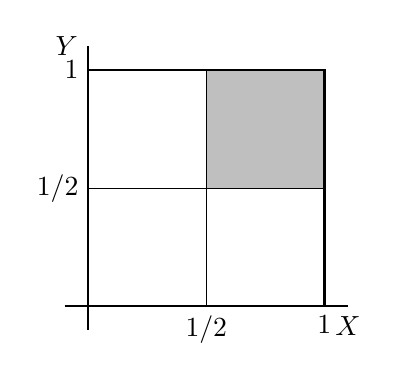
\begin{tikzpicture}[
    scale=3,
    %axis/.style={very thick, ->, >=stealth'},
    important line/.style={thick},
    dashed line/.style={dashed, thin},
    pile/.style={thick, ->, >=stealth', shorten <=2pt, shorten
    >=2pt},
    every node/.style={color=black}
    ]
    % axis
    \draw[thick] (-0.1,0)  -- (1.1,0) node(xline)[below]
        {$X$};
    \draw[thick] (0,-0.1) -- (0,1.1) node(yline)[left] {$Y$};
    % Values
    \draw (0,1) node(xline)[left]{$1$};
    \draw (0,0.5) node(xline)[left]{$1/2$};
    \draw (1,0) node(xline)[below]{$1$};
    \draw (0.5,0) node(xline)[below]{$1/2$};
    % Fill
    \fill[fill=gray!50] (0.5,0.5) -- (0.5,1) -- (1,1) -- (1,0.5) -- cycle;
    % Box
    \draw[important line] (0,0) -- (0,1) -- (1,1) -- (1,0) -- cycle;
    % Lines
    \draw (0.5,0) coordinate (A) -- (0.5,1);
    \draw (0,0.5) coordinate (C) -- (1,0.5);
\end{tikzpicture}  
\end{minipage}%
\begin{minipage}[t]{0.3\textwidth}
    \centering 
    %%%%%%%%%%%%%%%%%%%%%%%%%%%%%%%%%%%%%%% P(Z > 1/4)
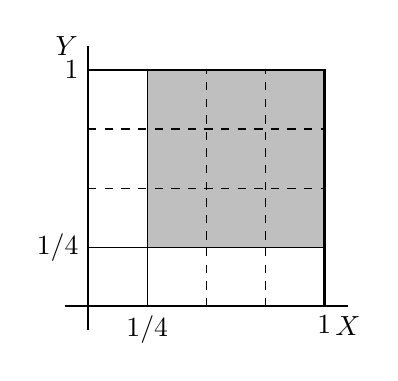
\begin{tikzpicture}[
    scale=3,
    %axis/.style={very thick, ->, >=stealth'},
    important line/.style={thick},
    dashed line/.style={dashed, thin},
    pile/.style={thick, ->, >=stealth', shorten <=2pt, shorten
    >=2pt},
    every node/.style={color=black}
    ]
    % axis
    \draw[thick] (-0.1,0)  -- (1.1,0) node(xline)[below]
        {$X$};
    \draw[thick] (0,-0.1) -- (0,1.1) node(yline)[left] {$Y$};
    % Values
    \draw (0,1) node(xline)[left]{$1$};
    \draw (0,0.25) node(xline)[left]{$1/4$};
    \draw (1,0) node(xline)[below]{$1$};
    \draw (0.25,0) node(xline)[below]{$1/4$};
    % Fill
    \fill[fill=gray!50] (0.25,0.25) -- (0.25,1) -- (1,1) -- (1,0.25) -- cycle;
    % Box
    \draw[important line] (0,0) -- (0,1) -- (1,1) -- (1,0) -- cycle;
    % Lines
    \draw (0.25,0) coordinate (A) -- (0.25,1);
    \draw[style=dashed] (0.5,0) coordinate (A) -- (0.5,1);
    \draw[style=dashed] (0.75,0) coordinate (A) -- (0.75,1);
    \draw (0,0.25) coordinate (C) -- (1,0.25);
    \draw[style=dashed] (0,0.5) coordinate (C) -- (1,0.5);
    \draw[style=dashed] (0,0.75) coordinate (C) -- (1,0.75);
\end{tikzpicture}
\end{minipage}%
\begin{minipage}[t]{0.3\textwidth}
    \centering
    %%%%%%%%%%%%%%%%%%%%%%%%%%%%%%%%%%%%%%% P(Z > 3/4)
    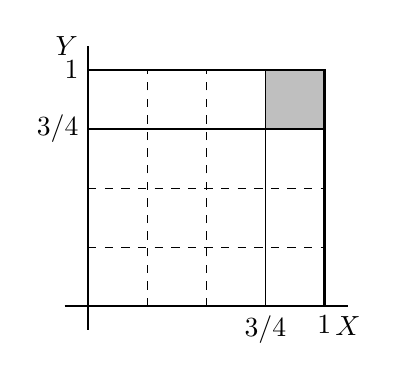
\begin{tikzpicture}[
        scale=3,
        %axis/.style={very thick, ->, >=stealth'},
        important line/.style={thick},
        dashed line/.style={dashed, thin},
        pile/.style={thick, ->, >=stealth', shorten <=2pt, shorten
        >=2pt},
        every node/.style={color=black}
        ]
        % axis
        \draw[thick] (-0.1,0)  -- (1.1,0) node(xline)[below]
            {$X$};
        \draw[thick] (0,-0.1) -- (0,1.1) node(yline)[left] {$Y$};
        % Values
        \draw (0,1) node(xline)[left]{$1$};
        \draw (0,0.75) node(xline)[left]{$3/4$};
        \draw (1,0) node(xline)[below]{$1$};
        \draw (0.75,0) node(xline)[below]{$3/4$};
        % Fill
        \fill[fill=gray!50] (0.75,0.75) -- (0.75,1) -- (1,1) -- (1,0.75) -- cycle;
        % Box
        \draw[important line] (0,0) -- (0,1) -- (1,1) -- (1,0) -- cycle;
        % Lines
        \draw[style=dashed] (0.25,0) coordinate (A) -- (0.25,1);
        \draw[style=dashed] (0.5,0) coordinate (A) -- (0.5,1);
        \draw (0.75,0) coordinate (A) -- (0.75,1);
        \draw[style=dashed] (0,0.25) coordinate (C) -- (1,0.25);
        \draw[style=dashed] (0,0.5) coordinate (C) -- (1,0.5);
        \draw (0,0.75) coordinate (C) -- (1,0.75);
    \end{tikzpicture}
\end{minipage}
\end{figure}
If we simulate lots of $X$ and $Y$ values, we see that about 1/4th of them will have both $X$ and
$Y$ values larger than 1/2, so $\P(Z>1/2) = 1/4$. Similarly, we get $\P(Z>1/4) = 9/16$ and
$\P(Z > 3/4) = 1/16$. Confirming this with a simulation.

\begin{lstlisting}[style=RSyntax]
# 2.7 - Simulating U(0,1)
N = 100000;X = runif(N);Y = runif(N)

Z = pmin(X, Y) # This is: Z = min{X, Y}

# Comparing simualted vs. theoretical results
sum(Z > 0.5)/N
1/4
sum(Z > 0.25)/N
9/16
sum(Z > 0.75)/N
1/16   
\end{lstlisting}
\begin{Verbatim}[fontsize=\small]
> # Comparing simualted vs. theoretical results
> sum(Z > 0.5)/N
[1] 0.24888
> 1/4
[1] 0.25

> sum(Z > 0.25)/N
[1] 0.56156
> 9/16
[1] 0.5625

> sum(Z > 0.75)/N
[1] 0.06205
> 1/16
[1] 0.0625
\end{Verbatim}

\newpage\noindent
By inspecting the images on the previous page, we can determine the 'shape' of the probabilities.
For $Z > 1/4$ we remove the union of $X \leq 1/4$ and $Y\leq 1/4$. We define $A = \{X \leq z\}$ and
$B = \{Y\leq z\}$, and can write the general case as:
\begin{align*}
    \P(Z > z) &=
    1 - \P(\{X \leq z\}\cup \{Y \leq z\}) \\
    &= 1 - \P(A\cup B) \\
    &= 1 - \big[\P(A) + \P(B) - \P(A\cap B)\big] \\
    &= 1 - \big[\P(A) + \P(B) - \P(A)\P(B)\big]
\end{align*}
Where we used Lemma 1.6, and the fact that $X$ and $Y$ are independent. By using the probability
law of complements, we can find the expression for $\P(Z\leq z)$.
$$
\P(Z\leq z) = \P(X\leq z) + \P(Y\leq z) - \P(X\leq z)\P(Y\leq z)
$$
The CDF for a uniform distribution on $U(a,b)$ is:
$$
F(z) = \frac{z-a}{b-a} \imp F_X(z) = F_Y(z) = \frac{z-0}{1-0} = z
$$
Which means:
$$
F_Z(z) = F_X(z) + F_Y(z) - F_X(z)F_Y(z) = 2z - z^2
$$
We can confirm our illustrations and simulated examples again by noting that:
\begin{align*}
    F_Z(1/2) &= \frac{1}{2} + \frac{1}{2} - \left(\frac{1}{2}\cdot\frac{1}{2}\right) = 1 - \frac{1}{4} = \frac{3}{4} \\
    F_Z(1/4) &= \frac{1}{4} + \frac{1}{4} - \left(\frac{1}{4}\cdot\frac{1}{4}\right) = \frac{8}{16} - \frac{1}{16} = \frac{7}{16}\\
    F_Z(3/4) &= \frac{3}{4} + \frac{3}{4} - \left(\frac{3}{4}\cdot\frac{3}{4}\right) = \frac{24}{16} - \frac{9}{16} = \frac{15}{16}
\end{align*}
which gives us the opposite results as expected (since we simulated and illustrated $\P(Z > z)$).
The PDF $f_Z(z)$ is the derivative of $F_Z(z)$.
Including PDF-plot and histogram of the simulated $Z$s.
$$
f_Z(z) = \frac{d}{dz}\Big(F_Z(z)\Big) = 2 - 2z.
$$
%Including a plot of the PDF as well as the histogram of the simulated $Z$ values.
\begin{figure}[H]
    \begin{minipage}{0.5\textwidth}
\begin{tikzpicture}
    \begin{axis}[
        width=0.8\textwidth,
        axis lines = left,
        ymin = -0.002,
        ymax = 2.1,
        xlabel = $z$,
        ylabel = {$f_Z(z)$},
    ]
    %Section 1
    \addplot [
        domain=0:1, 
        samples=10, 
        color=blue,
        style=ultra thick,
    ]
    {2 - 2*x};
    \end{axis}
\end{tikzpicture}
    \end{minipage}
    \begin{minipage}{0.5\textwidth}
        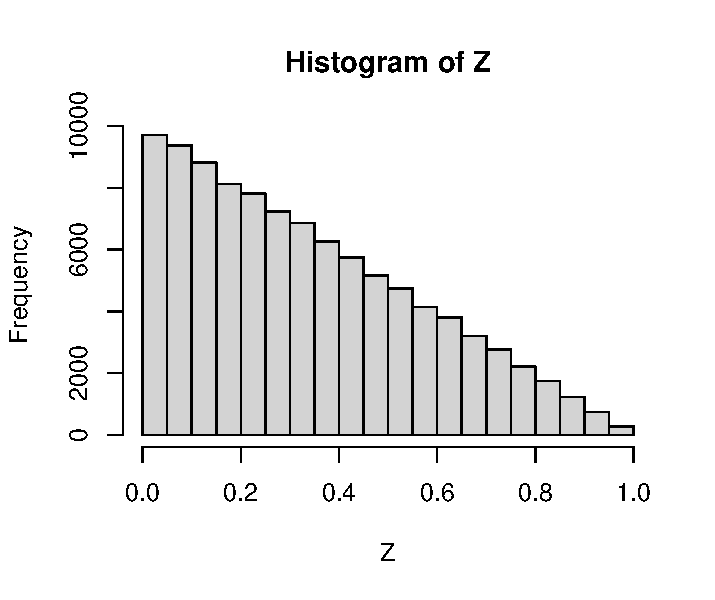
\includegraphics[scale=0.55]{ch2_2.7b.pdf}
    \end{minipage}
\end{figure}

\newpage\noindent
%%%%%%%%%%%%%%%%%%%%%%%%%%%%%%%%%%%%%%%%%%%%%%%%%%%%%%%%%%%%%%%%%%%%%%%%%%%%%%%
\textbf{2.8}\\  % PDF page 45
The RV $X$ has CDF $F$. Finding the CDF of $X^+ = \max\{0, X\}$.

\medskip\noindent
From the definition of CDF:
\begin{align*}
    F_{X^+}(u) &=  \P\big(\max(0, X)\leq u\big)\\
    &= \P\Big(\{\omega\in \Omega \;:\; X(\omega)\leq u\;\text{and}\; u\geq 0\}\Big)
\end{align*}
We must consider two cases. When $u < 0$:
\begin{align*}
    F_{X^+}(u) &= \P\Big(\{\omega\in \Omega \;:\; X(\omega)\leq u\;\text{and}\; u\geq 0\}\Big) \\
    &= \P(\emptyset) \\
    &= 0
\end{align*}
When $u\geq 0$:
\begin{align*}
    F_{X^+}(u) &= \P\Big(\{\omega\in \Omega \;:\; X(\omega)\leq u\;\text{and}\; u\geq 0\}\Big) \\
    &= \P\Big(\{\omega\in \Omega \;:\; X(\omega)\leq u\}\Big)  \\
    &= \P(X\leq u) \\
    &= F_X(u)
\end{align*}
So in summary:
$$
F_{X^+}(u) =
\left\{
    \begin{matrix}
        0 & u<0 \\
        F_X(u) & u\geq0 \\
    \end{matrix}
\right.
$$

% \medskip\noindent
% Illustration of what happens when we go from $X$ to $X^+$ for some continuous
% distribution, such as $X\sim N(0,1)$.
% \begin{figure}[H]
%     \begin{minipage}{0.5\textwidth}
% \begin{tikzpicture}
%     \begin{axis}[
%         width=\textwidth,
%         axis lines = left,
%         ymin = -0.002,
%         ymax = 0.5,
%         xlabel = $x$,
%         ylabel = {$f_X(x)$},
%     ]
%     %Section 1
%     \addplot [
%         domain=-2:2, 
%         samples=50, 
%         color=blue,
%         style=ultra thick,
%     ]
%     {1/(sqrt(2*3.1415))*exp(-0.5*x^2)};
%     \end{axis}
% \end{tikzpicture}
%     \end{minipage}
%     \begin{minipage}{0.5\textwidth}
%         \begin{tikzpicture}
%             \begin{axis}[
%                 width=\textwidth,
%                 axis lines = left,
%                 ymin = -0.002,
%                 ymax = 0.5,
%                 xlabel = $x$,
%                 ylabel = {$f_{X^+}(x)$},
%             ]
%             %Section 1
%             \addplot [
%                 domain=-2:0, 
%                 samples=2, 
%                 color=blue,
%                 style=ultra thick,
%             ]
%             {0};
%             %Section 2
%             \addplot [
%                 domain=0:2, 
%                 samples=50, 
%                 color=blue,
%                 style=ultra thick,
%             ]
%             {1/(sqrt(2*3.1415))*exp(-0.5*x^2)};
%             %Vertical lines
%             \addplot +[mark=none, color=blue] coordinates {(0, -0) (0, 0.4)};
%             \end{axis}
%         \end{tikzpicture}
%     \end{minipage}
% \end{figure}
% We split up the $X$ into negative and positive values, which becomes a disjoint set.
% $$
% \{X\leq x : x\in\R\} = 
% \{X\leq x : x\leq 0\} \cup \{0 < X\leq x : x>0\}
% $$
% Since they are disjoint:
% $$
% \P(X\leq x) = \P(X \leq 0) + \P(0<X\leq x) = F(0) + F(x) - F(0)
% $$
% We can split up the CDF:
% $$
% F(X\leq x) = F(X\leq 0)
% $$
% \medskip\noindent
% One of the defining properties of a PDF is that it must be greater than or equal to 0.
% Since the CDF if the integral of the PDF, it will always be greater than or equal to 0
% as well.
%%%% No, wait - this is incorrect. We could have e.g. U(-1, 1) or N(0, 1) in which case many
%%%% X will be negative. So the PDF is never negative, that is true, but that says
%%%% nothing about the X.

\bigskip\noindent
%%%%%%%%%%%%%%%%%%%%%%%%%%%%%%%%%%%%%%%%%%%%%%%%%%%%%%%%%%%%%%%%%%%%%%%%%%%%%%%
\textbf{2.9}\\  % PDF page 45
We have $X\sim \text{Exp}(\beta)$. The PDF is given by:
$$
f(x) = \frac{1}{\beta}e^{-x/\beta},\quad x > 0
$$
Finding the CDF by integrating the PDF.
\begin{align*}
    F(y) &= \int_{-\infty}^y f(x)dx \\
    &= \frac{1}{\beta}\int_0^y e^{-x/\beta}dx\\
    &= \frac{1}{\beta}\big[-\beta e^{-x/\beta}\big]_0^y\\
    &= \big[-e^{-x/\beta}\big]_0^y \\
    &= 1 - e^{-y/\beta}
\end{align*}
To find the inverse $F^{-1}(q)$ we set $q = F(y)$ and solve for $y$.
$$
q = 1 - e^{-y/\beta}
\imp
y = -\beta\log(1 - q)
\imp
F^{-1}(q) = -\beta\log(1 - q)
$$

\bigskip\noindent
%%%%%%%%%%%%%%%%%%%%%%%%%%%%%%%%%%%%%%%%%%%%%%%%%%%%%%%%%%%%%%%%%%%%%%%%%%%%%%%
\textbf{2.10}\\  % PDF page 45
If $X$ and $Y$ are independent, then $g(X)$ and $h(Y)$ are independent for some functions
$g$ and $h$.

\medskip\noindent
\textsc{Proof}.
Let $X$ and $Y$ be some arbitrary random variables, and let $x$ and $y$ be
values in the range of $g$ and $h$ such that $g(X) = x$ and $h(Y) = y$. Then:
\begin{align*}
    \P(g(X) = x, h(Y) = y) &=
    \P(X = g^{-1}(x), Y = h^{-1}(y)) \\
\shortintertext{By independence of $X$ and $Y$.}
&= \P(X = g^{-1}(x))\P(Y = h^{-1}(y)) \\
&= \P(g(X) = x)\P(h(Y) = y) 
\end{align*}
which shows that $g$ and $h$ satisfies the condition for independence.\qed
% When $X$ and $Y$ are independent, we want to show that the following is true:
% $$
% \P(g(X)\cap h(Y)) = \P(g(X))\P(h(Y))
% $$

\bigskip\noindent
%%%%%%%%%%%%%%%%%%%%%%%%%%%%%%%%%%%%%%%%%%%%%%%%%%%%%%%%%%%%%%%%%%%%%%%%%%%%%%%
\textbf{2.11}\\  % PDF page 45
Tossing a coin which has probability $p$ of getting H. We let $X$ denote the
number of heads and $Y$ the number of tails.

\medskip\noindent(a) Showing that $X$ and $Y$ are dependent. First it will be helpful
to consider a simplified case where we have $N=1$ and $N=2$ coin tosses, and assuming $p=1/2$.
\begin{figure}[H]
    \begin{minipage}{0.5\textwidth}
        $N = 1$ Tosses \\
        $$
            \begin{tabular}{c|c|c|c}
                & $Y=0$ & $Y=1$ & \\
                \hline
                $X=0$ & 0 & $1/2$ & $1/2$ \\
                \hline
                $X=1$ & $1/2$ & 0 & $1/2$ \\
                \hline
                & $1/2$ & $1/2$ & 1
            \end{tabular}
        $$
        \rule{0pt}{5pt}
    \end{minipage}
    \begin{minipage}{0.5\textwidth}
        $N = 2$ Tosses \\
        $$
            \begin{tabular}{c|c|c|c|c}
                & $Y=0$ & $Y=1$ & $Y=2$ & \\
                \hline
                $X=0$ & 0 & 0 & 1/4 & $1/4$ \\
                \hline
                $X=1$ & 0 & 1/2 & 0 & $1/2$ \\
                \hline
                $X=2$ & $1/4$ & 0 & 0 & $1/4$ \\
                \hline
                & $1/4$ & $1/2$ & $1/4$ & 1
            \end{tabular}
        $$
    \end{minipage}
\end{figure}
In the case of $N=2$, we see that $f(0, 2) = 1/4$ while $f_X(0)f_Y(2) = 1/16$. This will be the
inspiration for how we show it in the general case with $N$ tosses and probability $p$ of heads.

\medskip\noindent
We only need to show one specific case where $\P(X=x, Y=y) \not= \P(X=x)\P(Y=y)$ to show that these
values are dependent. The total number of tosses will be $N = X + Y$ and we compare the cases where
we get $N$ heads. In that case, using the Multinomial distribution:
$$
\P(X=N, Y=0) = {N\choose N,0} =p^N(1-p)^0 = p^N,
$$
but with the two Binomial distributions:
$$
\P(X=N)\P(Y=0) = {N\choose N}p^N(1-p)^0\times {N\choose 0}p^0(1-p)^N = p^N(1-p)^N.
$$
These are not equal, showing that $X$ and $Y$ are dependent variables.


\newpage\noindent
%%%%%%%%%%%%%%%%%%%%%%%%%%%%%%%%%%%%%%%%%%%%%%%%%%%%%%%%%%%%%%%%%%%%%%%%%%%%%%%
(b) Now we have $N\sim\text{Poisson}(\lambda)$, where $N = X + Y$ for $X$ heads
and $Y$ tails. Show that these values are now independent.

\medskip\noindent\emph{Current solution, but not sure it's correct...}\\
Assuming $X=x$ and $Y=y$. Then:
\begin{align*}
    \P(X=x\cap Y=y) &= \P(X=x\cap Y=y\cap N = x+y) \\
    &= \P(X=x\cap Y=y \mid N = x+y)\cdot\P(N = x+y) \\
    &= {x+y\choose x}p^x(1-p)^y\cdot e^{-\lambda}\frac{\lambda^{x+y}}{(x+y)!} \\
    &= \frac{\cancel{(x+y)!}}{x!y!}p^x(1-p)^y\cdot e^{-\lambda}\frac{\lambda^x\lambda^y}{\cancel{(x+y)!}} \\
    &= e^{-\lambda}\frac{p^x\lambda^x}{x!}\cdot\frac{(1-p)^y\lambda^y}{y!} \\
    &= e^{-\lambda p}\frac{p^x\lambda^x}{x!}\cdot e^{-\lambda(1-p)}\frac{(1-p)^y\lambda^y}{y!} \\
    &= \P(X=x | \lambda p)\cdot\P(Y=y|\lambda(1-p)) \\
    &= \P(X=x)\P(Y=y)
\end{align*}
Which shows we have independence. We used:
$$
e^{-\lambda} = e^{-\lambda(p - p + 1)} = e^{-\lambda p + \lambda p - \lambda}
= e^{-\lambda p}e^{\lambda p - \lambda} = e^{-\lambda p}e^{-\lambda(1-p)}.
$$
Also, we made the assumption that $\P(X=x\cap Y=y \mid N = x+y)$ is Binomial. But I think this is
only true when we can assume that $X$ and $Y$ are independent... which is what we are trying to show.
Will review this later... hopefully!

\bigskip\noindent
%%%%%%%%%%%%%%%%%%%%%%%%%%%%%%%%%%%%%%%%%%%%%%%%%%%%%%%%%%%%%%%%%%%%%%%%%%%%%%%
\textbf{2.12} \textsc{Theorem} 2.33\\  % PDF page 45
Suppose that the range of $X$ and $Y$ is a (possibly infinite)
rectangle. If $f(x, y) = g(x)h(y)$ for some functions $g$ and $h$ (not necessarily
probability density functions) then $X$ and $Y$ are independent.

\medskip\noindent\textsc{Proof}. From the joint PDF, we can find the marginal distributions:
$$
f_X(x) = \int f(x, y) dy, \quad
f_Y(y) = \int f(x, y) dx
$$
By applying these integrals to both sides of the equality:
$$
\int f(x, y) dy = g(x)\int h(y) dy \imp f_X(x) = g(x)
$$
$$
\int f(x, y) dx = h(y)\int g(x) dx \imp f_Y(y) = h(y)
$$
We get $g(x)$ and $h(y)$ since they are equal to $f(x,y)$ over the entire 'rectangle' and must therefore
integrate to 1. This leaves us with: $f(x, y) = g(x)h(y) = f_X(x)f_Y(y)$, and by the results in exercise 2.5,
this means that $X$ and $Y$ are independent. \qed

\newpage\noindent
%%%%%%%%%%%%%%%%%%%%%%%%%%%%%%%%%%%%%%%%%%%%%%%%%%%%%%%%%%%%%%%%%%%%%%%%%%%%%%%
\textbf{2.13}\\  % PDF page 45
(a) Finding the PDF of $Y = e^X$ when $X\sim N(0,1)$.
\begin{align*}
    F_Y(y) &= \P(Y\leq y) = \P(e^X \leq y) \\
    &= \P(X\leq \log(y)) = F_X(\log(y))
\end{align*}
We simply get the standard normal distribution back, but we input the logarithm of $y$.
This means we get the PDF:
$$
f_Y(y) = f_X(\log(y)) = \frac{1}{\sqrt{2\pi}}\exp\left(-\frac{1}{2}\big(\log(y)\big)^2\right)
$$
Plotting the function:
\begin{figure}[H]
\begin{minipage}{0.5\textwidth}
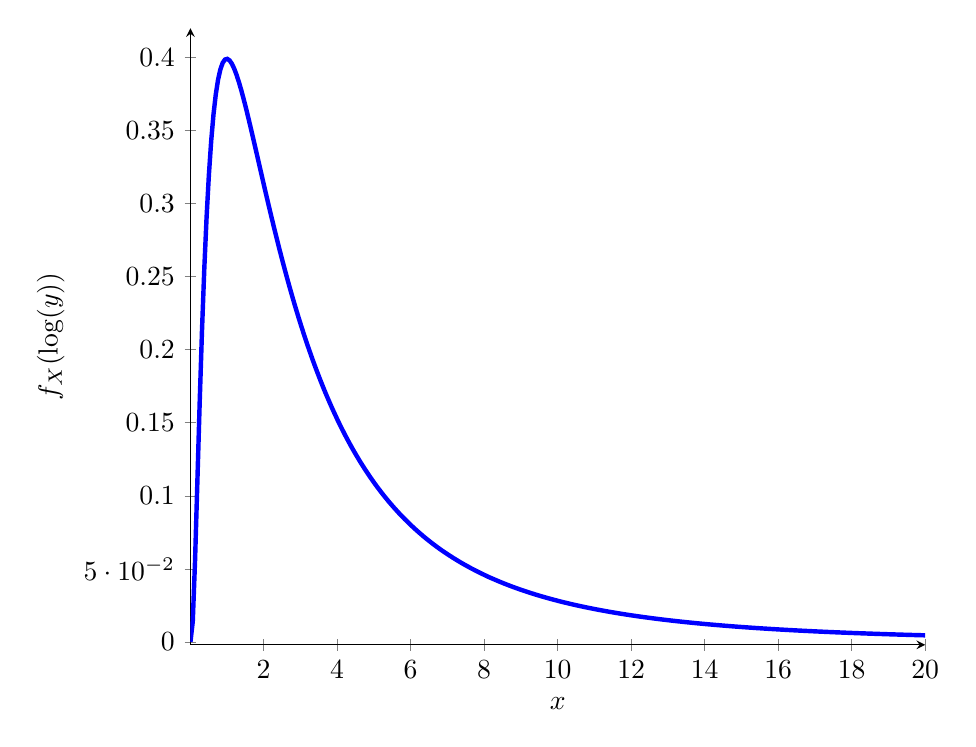
\begin{tikzpicture}
    \begin{axis}[
        width=0.9\textwidth,
        axis lines = left,
        ymin = -0.002,
        ymax = 0.42,
        xlabel = $x$,
        ylabel = {$f_X(\log(y))$},
    ]
    %Section 1
    \addplot [
        domain=-5:20, 
        %domain=-1:5, 
        samples=400, 
        color=blue,
        style=ultra thick,
    ]
    {(1/(sqrt(2*pi)))*exp(-0.5*ln(x)*ln(x))};
    \end{axis}
\end{tikzpicture}
\end{minipage}
\begin{minipage}{0.5\textwidth}
\end{minipage}
\end{figure}
(b) Plotting histogram of simulated results. Comparable to the plot above.
\begin{figure}[H]
    \begin{minipage}{0.5\textwidth}
        \begin{center}
            \begin{figure}[H]
            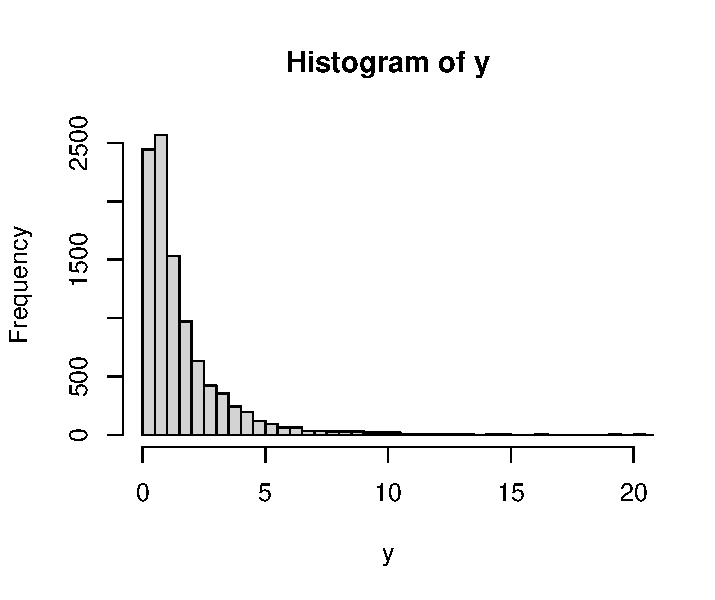
\includegraphics[scale=0.65]{ch2_2.13b.pdf}
            \end{figure}
        \end{center}
    \end{minipage}
    \begin{minipage}{0.5\textwidth}
    \begin{lstlisting}[style=RSyntax]
x = rnorm(10000)
y = exp(x)
hist(y, breaks = 100, xlim = c(0, 20))
pdf("~/AllStatistics/files/ch2_2.13b.pdf",
     width = 4.7747, height = 4)
hist(y, breaks = 100, xlim = c(0, 20))
dev.off()
    \end{lstlisting}
    \rule{0pt}{55pt}
\end{minipage}
\end{figure}






\begin{comment}

\bigskip\noindent
%%%%%%%%%%%%%%%%%%%%%%%%%%%%%%%%%%%%%%%%%%%%%%%%%%%%%%%%%%%%%%%%%%%%%%%%%%%%%%%
\textbf{2.X}\\  % PDF page 45


\begin{align*}
    A &= B
\end{align*}


\begin{equation*}
    A = B
    \tag*{\qed}
\end{equation*}


%%% Tikz Image - side by side
\begin{figure}
    \begin{minipage}[0.5\textwidth]
\begin{tikzpicture}
    \begin{axis}[
        width=\textwidth,
        axis lines = left,
        ymin = -0.002,
        ymax = 2.1,
        xlabel = $z$,
        ylabel = {$f_Z(z)$},
    ]
    %Section 1
    \addplot [
        domain=0:1, 
        samples=10, 
        color=blue,
        style=ultra thick,
    ]
    {2 - 2*x};
    \end{axis}
\end{tikzpicture}
    \end{minipage}
    \begin{minipage}[0.5\textwidth]
\begin{tikzpicture}
    \begin{axis}[
        width=\textwidth,
        axis lines = left,
        ymin = -0.002,
        ymax = 2.1,
        xlabel = $z$,
        ylabel = {$f_Z(z)$},
    ]
    %Section 1
    \addplot [
        domain=0:1, 
        samples=10, 
        color=blue,
        style=ultra thick,
    ]
    {2 - 2*x};
    \end{axis}
\end{tikzpicture}
    \end{minipage}
\end{figure}


\begin{lstlisting}[style=RSyntax, title=R]
# Code
\end{lstlisting}

\begin{verbatim}
# Output
\end{verbatim}


\end{comment}
%
\newpage
\section{Chapter 3 - Expectation}

\subsection*{Exercises}

\bigskip\noindent
%%%%%%%%%%%%%%%%%%%%%%%%%%%%%%%%%%%%%%%%%%%%%%%%%%%%%%%%%%%%%%%%%%%%%%%%%%%%%%%
\textbf{3.1}\\  % PDF page 58
Define $X$ as the wealth after $n$ games. The probability of winning and losing is the same
for each outcome so $p = 1/2$.
\begin{align*}
    \E[X] &= \frac{1}{2}\cdot 2c+ \frac{1}{2}\cdot \left(\frac{1}{2}\right)c
    = c + \frac{c}{4} = \frac{5}{4}c
\end{align*}
We expect to have $5/4\cdot c$ after $n$ games. We can also verify this result with a simulation
in \textbf{R}.
\begin{lstlisting}[style=RSyntax, title=R]
> games = sample(c(2, 0.5), size = 1000000, replace = TRUE)
> mean(games)
[1] 1.250973
> 5/4
[1] 1.25
\end{lstlisting}

\bigskip\noindent
%%%%%%%%%%%%%%%%%%%%%%%%%%%%%%%%%%%%%%%%%%%%%%%%%%%%%%%%%%%%%%%%%%%%%%%%%%%%%%%
\textbf{3.2}\\  % PDF page 59
\textbf{Claim}. $\V(X) = 0$ if and only if $\P(X = c) = 1$ for some constant $c$.

\medskip\noindent\textsc{Proof}.\\
$\Rightarrow)$ Set $c = \mu$ and assume $\V(X) = 0$, which means that
$$
%\E[(X - \mu)^2] = \E[X^2] - \mu^2 = 0
\E[(X - \mu)^2] = 0
\imp
%\E[X^2] = \mu^2
\int (x - \mu)^2dF(x) = 0.
$$
This can only be 0 when $x = \mu = c$ for the entire domain of $X$. Hence $\P(X = c) = 1$.

\medskip\noindent
$\Leftarrow)$ Assume $\P(X=c) = 1$. When calculating the expectation:
$$
\mu = \E[X] = \int c dF(x) = c
$$
When calculating the variance:
$$
\V(X) = \int (x - \mu)^2dF(x) = \int (c - c)^2dF(x) = 0,
$$
since $x = c$ for all $x$ in the domain of $X$. \qed

\newpage\noindent
%%%%%%%%%%%%%%%%%%%%%%%%%%%%%%%%%%%%%%%%%%%%%%%%%%%%%%%%%%%%%%%%%%%%%%%%%%%%%%%
\textbf{3.3}\\  % PDF page 59
Let $X_1,\ldots, X_n\sim U(0,1)$ and define $Y = \max(X_1,\ldots, X_n)$. We will calculate
$\E[Y]$. It is not stated in the exercise, but we will assume that the $X_i$ are independent.
Finding the CDF for $Y$.
\begin{align*}
    F_Y(y) &= \P(Y\leq y) \\
    &= \P(\max(X_1, \ldots, X_n) \leq y) \\
    &= \P(X_1\leq y)\cap\ldots\cap\P(X_n\leq y) \\
    &= \P(X_1\leq y)\P(X_2\leq y)\cdots\P(X_n\leq y) \tag{Independence}\\
    &= (F_X(y))^n
\end{align*}
Differentiating to get the PDF for $Y$.
$$
f_Y(y) = \frac{d}{dy}F_Y(y) = \frac{d}{dy}(F_X(y))^n = n(F_X(y))^{n-1}f_X(y)
$$
Since $X_i$ are uniformly distributed, we know that $F_X(y) = y$ and $f_X(y) = 1$, so:
$$
f_Y(y) = ny^{n-1}
$$
Now we can calculate the expectation of $Y$.
$$
\E[Y] = \int_0^1 y\cdot ny^{n-1} dy = n\int_0^1 y^n dy = n\Big[\frac{y^{n+1}}{n+1}\Big]_0^1 = \frac{n}{n+1}
$$
Confirming this result with a numeric simulation in \RR.

\begin{lstlisting}[style=RSyntax, title=R]
> # 3.3
> N = 1000000
> U1 = runif(N)
> U2 = runif(N)
> U3 = runif(N)
> U4 = runif(N)
> U5 = runif(N)
> U6 = runif(N)
> U7 = runif(N)
> U8 = runif(N)
> U9 = runif(N)
> U10 = runif(N)
> Y = pmax(U1, U2, U3, U4, U5,
+          U6, U7, U8, U9, U10)
> mean(Y)
[1] 0.9091151
> # Theoretical Result
> 10/11
[1] 0.9090909
\end{lstlisting}
As we can see, the theoretical result is very close to the simulated result for $n=10$.
% \begin{verbatim}
%     # Output
% \end{verbatim}
% # 3.3
% N = 1000000
% U1 = runif(N)
% U2 = runif(N)
% U3 = runif(N)
% U4 = runif(N)
% U5 = runif(N)
% U6 = runif(N)
% U7 = runif(N)
% U8 = runif(N)
% U9 = runif(N)
% U10 = runif(N)
% Y = pmax(U1, U2, U3, U4, U5,
%          U6, U7, U8, U9, U10)
% mean(Y)
% # Theoretical Result n/(n+1)
% 10/11

\newpage\noindent
%%%%%%%%%%%%%%%%%%%%%%%%%%%%%%%%%%%%%%%%%%%%%%%%%%%%%%%%%%%%%%%%%%%%%%%%%%%%%%%
\textbf{3.4} - Random Walk\\  % PDF page 59
A particle starts in the origin and jumps left, a step of -1, with probability $p$
and jumps right, a step of 1, with probability $1-p$. The expected location will be:
$$
\E[X] = (-1)p + (1)(1-p) = -p + 1 - p = 1 - 2p
$$
To calculate the variance, we start by finding the second moment:
$$
\E[X^2] = (-1)^2p + (1)^2(1-p) = p + 1 - p = 1
$$
So the variance is:
$$
\V(X) = \E[X^2] - \E[X]^2 = 1 - (1 - 2p)^2 = 1 -(1 - 4p + 4p^2) = 4p - 4p^2
$$

\bigskip\noindent
%%%%%%%%%%%%%%%%%%%%%%%%%%%%%%%%%%%%%%%%%%%%%%%%%%%%%%%%%%%%%%%%%%%%%%%%%%%%%%%
\textbf{3.5}\\  % PDF page 59
Tossing a fair coin until we get H. Finding the expected number of tosses. The reasoning is
as follows. We get H on the first toss with probability 1/2, first H on the second toss
with probability $1/2^2$ = 1/4 and so on. The pattern becomes as follows, for the first 7 cases:
$$
\begin{tabular}{lll}
    \textbf{Tosses} & \textbf{Outcome} & \textbf{Probability} \\
    1 & $\{H\}$ & 1/2 \\
    2 & $\{TH\}$ & 1/4 \\
    3 & $\{TTH\}$ & 1/8 \\
    4 & $\{TTTH\}$ & 1/16 \\
    5 & $\{TTTTH\}$ & 1/32 \\
    6 & $\{TTTTTH\}$ & 1/64 \\
    7 & $\{TTTTTTH\}$ & 1/128
\end{tabular}
$$
Define $T$ to be the number of tosses to get H.
\begin{align*}
    \E[T] &= (1)\left(\frac{1}{2}\right) + (2)\left(\frac{1}{4}\right) + \ldots + (k)\left(\frac{1}{2^k}\right) + \ldots \\
    &= \sum_{k=1}^\infty \frac{k}{2^k} \\
    &= 2
\end{align*}
Not delving in to the mathematics of the infinite sum, but it can be shown that this sum becomes 2
which will be the expected number of tosses to get a H. Here is a numeric approximation in \RR.
\begin{lstlisting}[style=RSyntax, title=R]
> sumApprox = 0
> for (k in 1:1000) {
+   sumApprox = sumApprox + k/2^k
+ } 
> sumApprox
[1] 2
\end{lstlisting}

\newpage\noindent
%%%%%%%%%%%%%%%%%%%%%%%%%%%%%%%%%%%%%%%%%%%%%%%%%%%%%%%%%%%%%%%%%%%%%%%%%%%%%%%
\textbf{3.6} \textbf{Theorem} - The Rule of the Lazy Statistician\\  % PDF page 59
Proving the following result for the discrete case. Let $Y = r(X)$, then
$$
\E[Y] = \E[r(X)] = \sum_{x}r(x)f(x)
$$
\textsc{Proof}.








\begin{comment}

\bigskip\noindent
%%%%%%%%%%%%%%%%%%%%%%%%%%%%%%%%%%%%%%%%%%%%%%%%%%%%%%%%%%%%%%%%%%%%%%%%%%%%%%%
\textbf{3.X}\\  % PDF page 59


\begin{align*}
    A &= B
\end{align*}


\begin{equation*}
    A = B
    \tag*{\qed}
\end{equation*}


\begin{lstlisting}[style=RSyntax, title=R]
# Code
\end{lstlisting}

\begin{verbatim}
# Output
\end{verbatim}




%%% Tikz Image - side by side
\begin{figure}
    \begin{minipage}[0.5\textwidth]
\begin{tikzpicture}
    \begin{axis}[
        width=\textwidth,
        axis lines = left,
        ymin = -0.002,
        ymax = 2.1,
        xlabel = $z$,
        ylabel = {$f_Z(z)$},
    ]
    %Section 1
    \addplot [
        domain=0:1, 
        samples=10, 
        color=blue,
        style=ultra thick,
    ]
    {2 - 2*x};
    \end{axis}
\end{tikzpicture}
    \end{minipage}
    \begin{minipage}[0.5\textwidth]
\begin{tikzpicture}
    \begin{axis}[
        width=\textwidth,
        axis lines = left,
        ymin = -0.002,
        ymax = 2.1,
        xlabel = $z$,
        ylabel = {$f_Z(z)$},
    ]
    %Section 1
    \addplot [
        domain=0:1, 
        samples=10, 
        color=blue,
        style=ultra thick,
    ]
    {2 - 2*x};
    \end{axis}
\end{tikzpicture}
    \end{minipage}
\end{figure}


\end{comment}
%
\newpage
\section{Inequalities}

\subsection*{Practical Example}
\textbf{Example 1 - Markov's Inequality}.\\
You hear that the mean age of NYU students is 20 years, but you know quite a few
students that are older than 30. You decide to apply Markov's inequality to bound
the fraction of students above 30 by modeling age as a nonnegative random variable A.
$$
\P(A > 30) \leq \frac{\E[A]}{30} = \frac{2}{3},
$$
so at most two thirds of the students are over 30.
This isn't a very precise bound, but then we also only use the expectation.

\medskip\noindent
\textbf{Example 2 - Chebyshev's Inequality}.\\
The previous bound is a little too weak. After investigating we discover that the
standard deviation of student age is actually just 3 years. Applying Chebyshev's
inequality to this information and obtain
$$
\P(|A - \E[A]| > 10) \leq \frac{\V(A)}{100} = \frac{9}{100}.
$$
So at least 91\% of the students are under 30 years old (and above 10).

\subsection*{Exercises}
%%%%%%%%%%%%%%%%%%%%%%%%%%%%%%%%%%%%%%%%%%%%%%%%%%%%%%%%%%%%%%%%%%%%%%%%%%%%%%%
\textbf{4.1}\\  % PDF page 68
Let $X\sim\text{Exp}(\beta)$. As we found in exercise 3.12, $\mu = \E[X] = \beta$ and
$\sigma^2 = \V(X) = \beta^2$. By applying Chebyshev's inequality:
$$
\P(|X-\beta|\geq t) = \P(|X-\mu|\geq t) \leq \frac{\sigma^2}{t^2} = \frac{\beta^2}{t^2}
$$
We are going to compare Chebyshev's inequality with the following inequality. Since $\sigma\geq 0$
and $k > 1$, we can apply Markov's inequality to get:
$$
\P(|X-\mu|\geq k\sigma) = \P((X-\mu)^2\geq k^2\sigma^2) \leq
\frac{\E[(X-\mu)^2]}{k^2\sigma^2} = \frac{\sigma^2}{k^2\sigma^2} = \frac{1}{k^2}
$$
We recognize this as the corollarly to the Chebyshev inequality. Comparing,
and using that $\sigma = \beta$, and using $t$ instead of $k$:
\begin{align*}
    \P(|X-\beta|\geq t) &\leq \frac{\beta^2}{t^2} \\
    \P(|X-\beta|\geq t\beta) &\leq \frac{1}{t^2}
\end{align*}
If $\beta > 1$, the first bound becomes 'weaker' which makes sense since $\beta t > t$ and
we are considering a smaller interval. If $\beta < 1$ the reverse is true. Also interesting
to note that by scaling up the bounded interval by $\beta$ gives a $\beta^2$ increase in the
bound, provided that $\beta > 1$. Shows there is a nonlinear relationship for the bound
when using the Exponential distribution.

\newpage\noindent
%%%%%%%%%%%%%%%%%%%%%%%%%%%%%%%%%%%%%%%%%%%%%%%%%%%%%%%%%%%%%%%%%%%%%%%%%%%%%%%
\textbf{4.2}\\  % PDF page 68
Let $X\sim\text{Poisson}(\lambda)$. As seen, $\E[X] = \lambda$ and
$\V(X) = \lambda$. Applying Chebyshev's inequality to show that
$\P(X\geq 2\lambda) = 1/\lambda$.
$$
\P(X \geq 2\lambda) = \P(X - \lambda \geq \lambda) \leq
\P(|X - \lambda| \geq \lambda) \leq \frac{\lambda}{\lambda^2} = \frac{1}{\lambda}.
$$
Which shows that $\P(X \geq 2\lambda) \leq 1/\lambda$.

\bigskip\noindent
%%%%%%%%%%%%%%%%%%%%%%%%%%%%%%%%%%%%%%%%%%%%%%%%%%%%%%%%%%%%%%%%%%%%%%%%%%%%%%%
\textbf{4.3}\\  % PDF page 68
Let $X_1,\ldots,X_n\sim\text{Bernoulli}(p)$ and define
$$
\bar{X} = \frac{1}{n}\sum_{i=1}^nX_i.
$$
Bound $\P(|\bar{X} - p| > \epsilon)$ with Chebyshev's and
Hoeffding's inequality. Show that when $n$ is large, the
Hoeffding's bound is smaller than Chebyshev's bound. (Assuming $\epsilon > 0)$.

For the Bernoulli distribution, $\E[X_i] = p$ and $\V(X_i) = p(1-p)$.
Since we are using a statistic, $\E[\bar{X}] = p$ and $\V(\bar{X}) = p(1-p)/n$
as per Theorem 3.17. Applying Chebyshev's inequality:
$$
\P(|\bar{X} - p| > \epsilon) \leq \frac{p(1-p)/n}{\epsilon^2} = \frac{p(1-p)}{n\epsilon^2}
\leq \frac{1/4}{n\epsilon^2} = \frac{1}{4n\epsilon^2}
$$
(Using that the max value of $p-p^2$ is 1/4 for $p\in(0,1)$).
Applying Hoeffding's inequality via Theorem 4.5.
$$
\P(|\bar{X} - p| > \epsilon) \leq 2e^{-2n\epsilon^2} = \frac{2}{e^{2n\epsilon^2}}
$$
To examine what happens as $n$ grows, we divide the Hoeffding bound by the Chebyshev bound
and call it $L_n$:
$$
L_n = 
\left(\frac{2}{e^{2n\epsilon^2}}\right)
\Big/
\left(\frac{1}{4n\epsilon^2}\right)
= \frac{8n\epsilon^2}{e^{2n\epsilon^2}}
$$
If we take the limit when $n\ra\infty$, both the numerator and denominator diverges.
So we apply L'Hôpital's rule and differentiate the numerator and denominator wrt. $n$:
$$
\lim_{n\ra\infty} L_n = 
\lim_{n\ra\infty} \frac{8n\epsilon^2}{e^{2n\epsilon^2}} = 
\lim_{n\ra\infty} \frac{8\epsilon^2}{2\epsilon^2e^{2n\epsilon^2}} = 0
$$
Since we lose the dependence on $n$ in the numerator, the fraction goes to 0 as $n$ grows.
So as $n$ becomes large, $L_n$ becomes 0, which means that the Hoeffding bound becomes
smaller than the Chebyshev bound.

\newpage\noindent
%%%%%%%%%%%%%%%%%%%%%%%%%%%%%%%%%%%%%%%%%%%%%%%%%%%%%%%%%%%%%%%%%%%%%%%%%%%%%%%
\textbf{4.4}\\  % PDF page 68
Let $X_1,\ldots,X_n\sim\text{Bernoulli}(p)$. 

\medskip\noindent(a) For some $\alpha > 0$, define:
$$
\epsilon = \sqrt{\frac{1}{2n}\log\left(\frac{2}{\alpha}\right)}
\imp
\epsilon^2 = \frac{1}{2n}\log\left(\frac{2}{\alpha}\right)
$$
and set $\hat{p} = n^{-1}\sum_{i=1}^n X_i$. Now we define
$C_n = (\hat{p} - \epsilon, \hat{p} + \epsilon)$ and will show that the probability that
$C_n$ contains $\hat{p}$ is $\alpha - 1$, using Hoeffding's inequality.

$C_n$ containing $p$ means that:
$$
p \in C_n \imp
\hat{p} - \epsilon \leq p \leq \hat{p} + \epsilon
\imp
-\epsilon \leq p - \hat{p} \leq \epsilon
\imp
|\hat{p} - p| \leq \epsilon
$$
where we used that $|\hat{p} - p| = |p - \hat{p}|$ in the final step. So:
$$
\P(p\in C_n) = \P(|\hat{p} - p| \leq \epsilon) = 1 - \P(|\hat{p} - p| > \epsilon)
$$
(the probability that $p$ is in the interval $C_n$ is equal to 1 minus the probability
that is outside the interval, basically). We can use the bound found in Theorem 4.5 again.
\begin{align*}
    \P(|\hat{p} - p| > \epsilon) &\leq
    2\exp\left\{-2n\epsilon^2\right\} \\
    &= 2\exp\left\{-2n\cdot\frac{1}{2n}\log\left(\frac{2}{\alpha}\right)\right\} \\
    &= 2\exp\left\{-\log\left(\frac{2}{\alpha}\right)\right\} \\
    &= 2\exp\left\{\log\left(\frac{\alpha}{2}\right)\right\}\\
    &= 2\left(\frac{\alpha}{2}\right) \\
    &= \alpha
\end{align*}
Rewriting this inequality in terms of $1-\alpha$.
\begin{align*}
    \P(|\hat{p} - p| > \epsilon) &\leq \alpha \\
    1 + \P(|\hat{p} - p| > \epsilon) &\leq 1 + \alpha \\
    1 - \alpha &\leq 1 - \P(|\hat{p} - p| > \epsilon)
\end{align*}
Which shows the desired result:
$$
1 - \alpha \leq 1 - \P(|\hat{p} - p| > \epsilon) = \P(p\in C_n).
$$
(b) Running some simulations. Doing 1000 simulations for $n=10, 50, 100, 2000$
and checking how often the $p$ lies in the range $\hat{p}\pm\epsilon$.

See code and plots on the next page.

\newpage\noindent

\begin{lstlisting}[style=RSyntax, title=R]
# 4.4(b): p = 0.4, alpha = 0.05
simBern <- function(n) {  # Simulate Bernoulli
    NSIM = 1000 # Do 1000 simulations per n
    simulationList = matrix(rep(0, n*NSIM), nrow = NSIM)
    for (i in 1:NSIM) {
        simulationList[i,1:n] = sample(c(1, 0), size=n,
                                       replace = TRUE, prob = c(0.4, 0.6))
    }
    return(simulationList)
} 
countCoverage <- function(sim, alpha) {
    N = ncol(sim); NSIM = nrow(sim)
    covRate = rep(0, NSIM)
    for (i in 1:NSIM) {
        mn = mean(sim[i, 1:N])
        if(abs(0.4 - mn) < 0.05) {
            covRate[i] = 1 
        }
    } 
    hitRate = sum(covRate)/NSIM;print(hitRate)
} 
# Bernoulli simulations
bsim10 = simBern(10);bsim50 = simBern(50)
bsim100 = simBern(100);bsim2000 = simBern(2000)
> countCoverage(bsim10, alpha=0.05)
[1] 0.268
> countCoverage(bsim50, alpha=0.05)
[1] 0.552
> countCoverage(bsim100, alpha=0.05)
[1] 0.684
> countCoverage(bsim2000, alpha=0.05)
[1] 1
\end{lstlisting}
Plotting the coverage rate vs. $n$. As $n$ increases, the interval will contain $p$ more often.
\begin{figure}[H]
    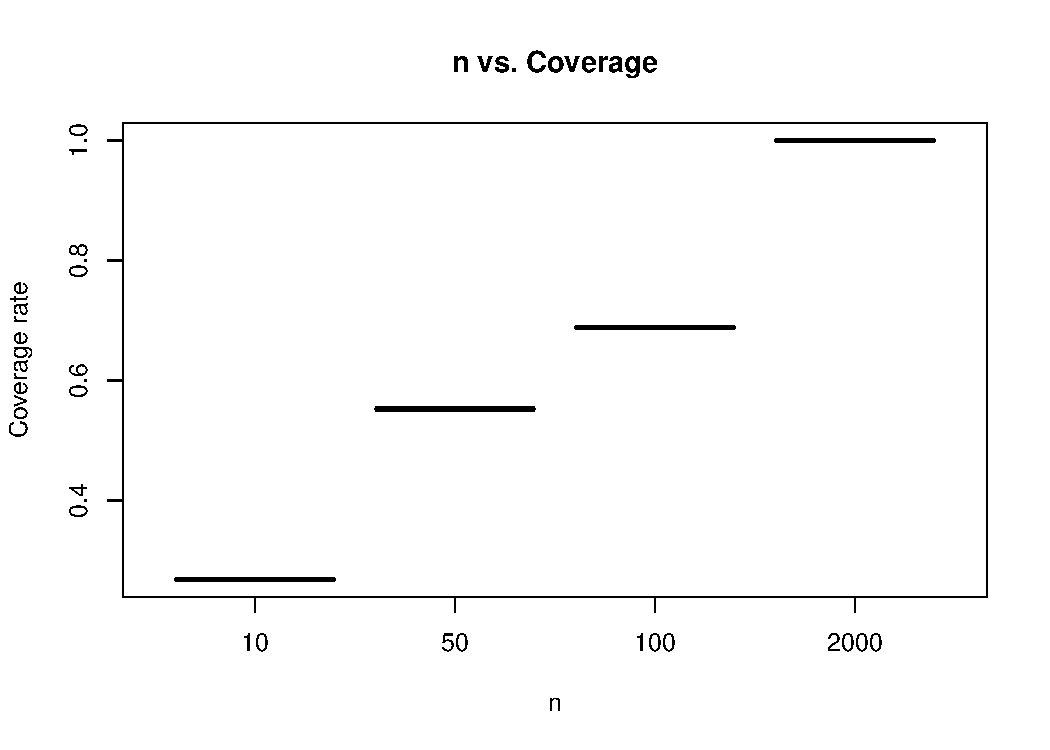
\includegraphics[scale=0.54]{ch4_4.pdf}
\end{figure}

\newpage\noindent
(c) Investigating the relationship between $n$ and the interval length:
$2|\hat{p} - p|$. When does it become smaller than 0.05? According to the simulation
results, that happens roughly when $n$ passes 200, based on our 1000-per-$n$ simulation.
\begin{lstlisting}[style=RSyntax, title=R]
# 4.4(c): Plotting length of interval
IntervalLength <- function(sim) {
    N = ncol(sim); NSIM = nrow(sim)
    intLength = rep(0, NSIM)
    for (i in 1:NSIM) {
        mn = mean(sim[i, 1:N])
        intLength[i] = 2*abs(0.4 - mn) 
    } 
    print(mean(intLength))
} 
> IntervalLength(bsim10)
[1] 0.2408
> IntervalLength(bsim50)
[1] 0.10572
> IntervalLength(bsim100)
[1] 0.077
> IntervalLength(bsim200)
[1] 0.0547
> IntervalLength(bsim300)
[1] 0.04543333
> IntervalLength(bsim2000)
[1] 0.017746
\end{lstlisting}
\begin{figure}[H]
    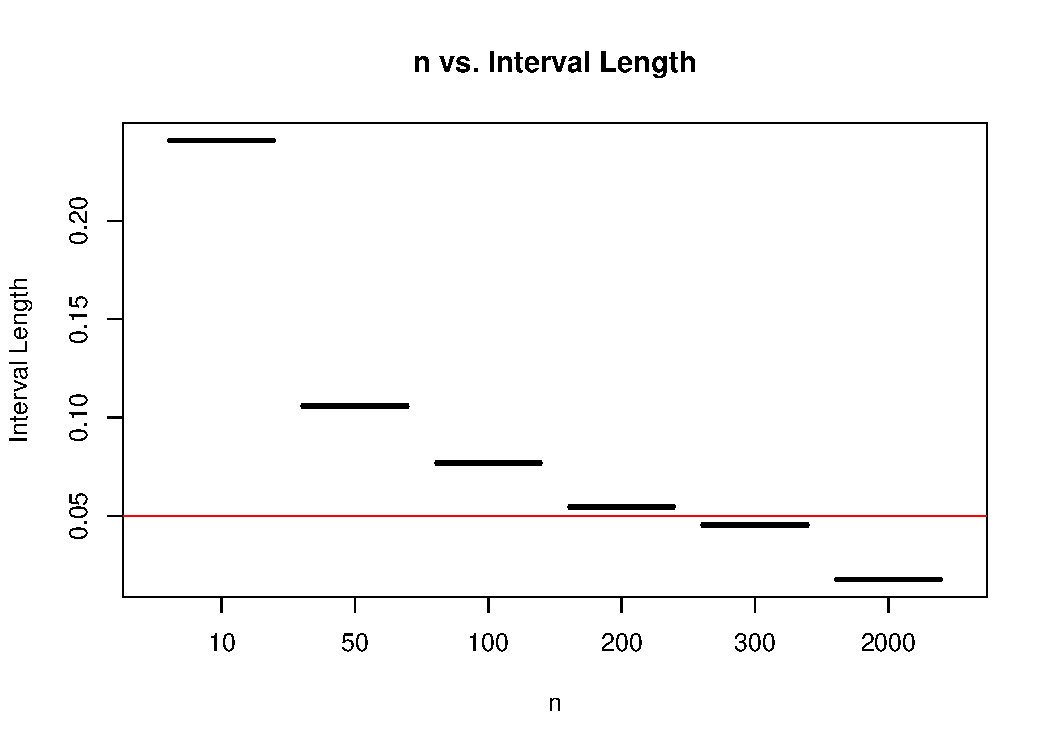
\includegraphics[scale=0.7]{ch4_4b.pdf}
\end{figure}

\newpage\noindent
%%%%%%%%%%%%%%%%%%%%%%%%%%%%%%%%%%%%%%%%%%%%%%%%%%%%%%%%%%%%%%%%%%%%%%%%%%%%%%%
\textbf{4.5} - Theorem 4.7: Mill's Inequality\\  % PDF page 68
Let $Z\sim N(0,1)$ and $t>0$. Then,
$$
\P(|Z| > t) \leq \sqrt{\frac{2}{\pi}}\cdot\frac{e^{-t^2/2}}{t}.
$$
\textsc{Proof}. From the hint, we can use the symmetry property of the normal
distribution, and when $t > 0$:
$$
\P(|Z| > t) = 2\P(Z > t)
\imp
\frac{1}{2}\P(|Z| > t) = \P(Z > t)
\imp
\frac{t}{2}\P(|Z| > t) = t\P(Z > t)
$$
As laid out in the proof of the Markov inequality, we get:
$$
\frac{t}{2}\P(|Z| > t) = t\P(Z > t) = t\int_t^\infty f(x)dx \leq \int_t^\infty xf(x)dx = I
$$
Calculating the integral $I$:
$$
I = \int_t^\infty xf(x)dx =
\frac{1}{\sqrt{2\pi}}\int_t^\infty x\cdot e^{-x^2/2}dx =
\frac{1}{\sqrt{2\pi}}\big[-e^{-x^2/2}\big]_t^\infty = \frac{1}{\sqrt{2\pi}}\Big(0 - (-e^{-t^2/2})\Big)
= \frac{1}{\sqrt{2\pi}}e^{-t^2/2}
$$
Collecting our findings:
$$
\frac{t}{2}\P(|Z| > t) \leq \frac{1}{\sqrt{2\pi}}e^{-t^2/2}
\imp
\P(|Z| > t) \leq \sqrt{\frac{2}{\pi}}\frac{e^{-t^2/2}}{t}
$$
which concludes the proof.\qed

\medskip\noindent
An additional note on the fraction manipulation.
$$
\frac{2}{\sqrt{2\pi}} = \frac{\sqrt{2}\sqrt{2}}{\sqrt{2}\sqrt{\pi}} = \frac{\sqrt{2}}{\sqrt{\pi}} = \sqrt{\frac{2}{\pi}}
$$


\bigskip\noindent
%%%%%%%%%%%%%%%%%%%%%%%%%%%%%%%%%%%%%%%%%%%%%%%%%%%%%%%%%%%%%%%%%%%%%%%%%%%%%%%
\textbf{4.6}\\  % PDF page 68
Let $Z\sim N(0,1)$. We simulate the probability that $\P(|Z| > t)$ and plot the results.
See code and plot on next page.

We will also include the Markov bounds. Since the Markov inequality only applies to
nonnegative random variables, we use it on $|Z|$. Finding $\E[|Z|]$ by using that
the standard normal distribution is symmetric, so we multiply the expected value for
$\E[Z > 0]$ by 2.
\begin{align*}
    \E[|Z|] &= 2\left(\frac{1}{\sqrt{2\pi}}\int_0^\infty x\cdot e^{-x^2/2}dx \right) \\
    &= \sqrt{\frac{2}{\pi}}\Big[-e^{-x^2/2}\Big]_0^\infty \\
    &= \sqrt{\frac{2}{\pi}}\Big(0 - ( - 1)\Big) \\
    &= \sqrt{\frac{2}{\pi}}
\end{align*}
(This can easily be verified numerically).

\newpage\noindent
\begin{lstlisting}[style=RSyntax, title=R]
# Plotting P(Z > t) as a function of t
Z = rnorm(1000000)
t = 1:2000/400 # t goes from 0 to 5
P_Zgt = rep(0, length(t))

for (i in 1:length(t)) {
    P_Zgt[i] = sum(abs(Z) > t[i])
} 
plot(t, P_Zgt/1e6, type="l",
     main="P(|Z|>t) for t in (0,5)")
\end{lstlisting}
Results from plot, when including bounds for the Markov and Hill inequalities:\\
\begin{figure}[H]
    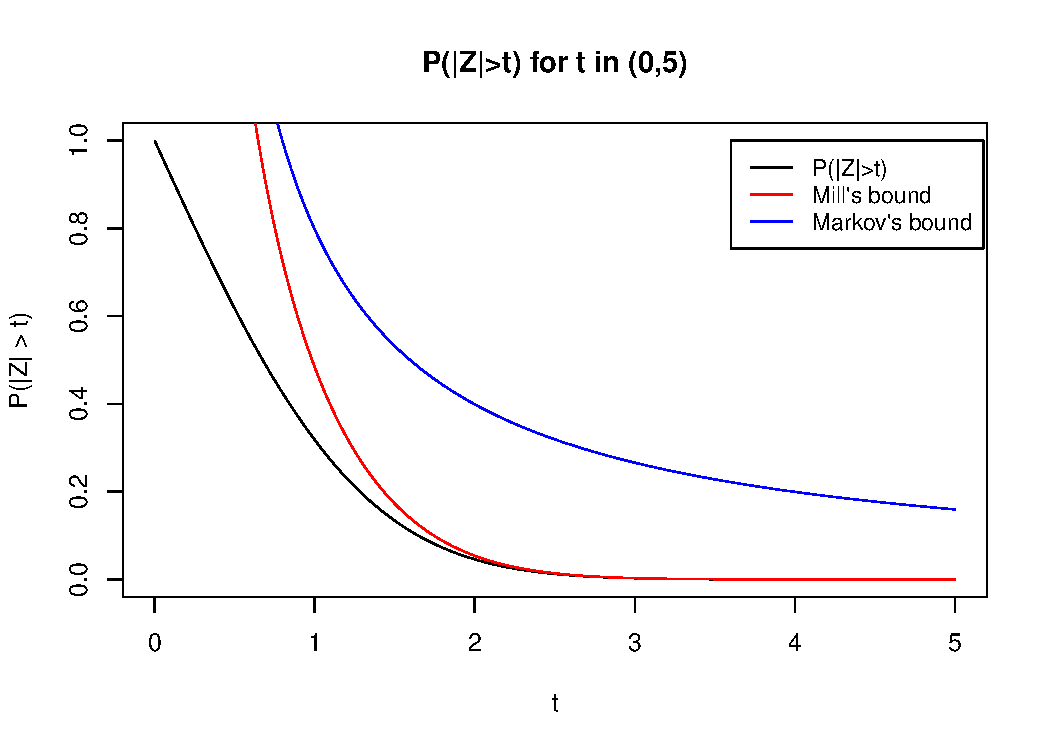
\includegraphics[scale=0.85]{ch4_6.pdf}
\end{figure}
The Markov inequality gives a very lose bound, but as we can see the Mill inequality
gives a bound that really hugs the $\P(|Z| > z)$ curve.

\newpage\noindent
%%%%%%%%%%%%%%%%%%%%%%%%%%%%%%%%%%%%%%%%%%%%%%%%%%%%%%%%%%%%%%%%%%%%%%%%%%%%%%%
\textbf{4.7}\\  % PDF page 68
Let $X_1,\ldots, X_n \sim N(0,1)$. Bound $\P(|\bar{X}| > t)$ using Mill's inequality,
where $\bar{X} = n^{-1}\sum_{i=1}^n X_i$ and compare to Chebyshev's bound.

We begin by applying the Chebyshev's inequality. The sampling distribution of $\bar{X}$
gives $\E[\bar{X}] = 0$ and $\V(\bar{X}) = \sigma^2/n = 1/n$. 
$$
\P(|\bar{X}| > t) = \P(|\bar{X} - \mu| > t) \leq \frac{\sigma^2}{t^2} = \frac{1}{nt^2}
$$
Now, the variable $\bar{X}$ no longer has a standard normal distribution, as we noted above.
We have $\bar{X} \sim N(0, 1/n)$. But we can do the following, since we only require $t > 0$:
\begin{align*}
    \P(|X| > t) &= \P(|0 + (1/n)Z| > t) \\
    &= \P(1/n|Z| > t)\\
    &= \P(|Z| > nt)
\end{align*}
So, by defining $k=nt > 0$, we get:
$$
\P(|X|>t) = \P(|Z| > k) \leq
\sqrt{\frac{2}{\pi}}\frac{e^{-k^2/2}}{k} =
\sqrt{\frac{2}{\pi}}\frac{e^{-(nt)^2/2}}{nt}
$$
No particular observations, except that we can note Hill's inequality relies on the square
of $n$, while Chebyshev's bound only uses $n$. By taking the limit and applying L'Hôpital's
rule, we can easily see that Hill's bound will be smaller as $n$ grows.









\begin{comment}

\bigskip\noindent
%%%%%%%%%%%%%%%%%%%%%%%%%%%%%%%%%%%%%%%%%%%%%%%%%%%%%%%%%%%%%%%%%%%%%%%%%%%%%%%
\textbf{4.X}\\  % PDF page 68


\begin{align*}
    A &= B
\end{align*}


\begin{equation*}
    A = B
    \tag*{\qed}
\end{equation*}


\begin{lstlisting}[style=RSyntax, title=R]
# Code
\end{lstlisting}

\begin{verbatim}
# Output
\end{verbatim}






%%%%%%%%%%%%%%%%%%%%%%%%%%%%%%%%%%%%%%%%%%% Minipages x 2
\begin{figure}[H]
    \begin{minipage}{0.5\textwidth}
        % MINIPAGE 1
    \end{minipage}
    \begin{minipage}{0.5\textwidth}
        % MINIPAGE 2
    \end{minipage}
\end{figure}

%%%%%%%%%%%%%%%%%%%%%%%%%%%%%%%%%%%%%%%%%%% Two R images
\begin{figure}[H]
    \begin{minipage}{0.5\textwidth}
    \begin{center}
        \begin{figure}[H]
            \includegraphics[scale=0.7]{IMG1.pdf}
        \end{figure}
    \end{center}
    \end{minipage}
    \begin{minipage}{0.5\textwidth}
    \begin{center}
        \begin{figure}[H]
            \includegraphics[scale=0.7]{IMG2.pdf}
        \end{figure}
    \end{center}
    \end{minipage}
\end{figure}


%%%%%%%%%%%%%%%%%%%%%%%%%%%%%%%%%%%%%%%%%%% Two TikZ images
%%% Tikz Image - side by side
\begin{figure}
    \begin{minipage}[0.5\textwidth]
\begin{tikzpicture}
    \begin{axis}[
        width=\textwidth,
        axis lines = left,
        ymin = -0.002,
        ymax = 2.1,
        xlabel = $z$,
        ylabel = {$f_Z(z)$},
    ]
    %Section 1
    \addplot [
        domain=0:1, 
        samples=10, 
        color=blue,
        style=ultra thick,
    ]
    {2 - 2*x};
    \end{axis}
\end{tikzpicture}
    \end{minipage}
    \begin{minipage}[0.5\textwidth]
\begin{tikzpicture}
    \begin{axis}[
        width=\textwidth,
        axis lines = left,
        ymin = -0.002,
        ymax = 2.1,
        xlabel = $z$,
        ylabel = {$f_Z(z)$},
    ]
    %Section 1
    \addplot [
        domain=0:1, 
        samples=10, 
        color=blue,
        style=ultra thick,
    ]
    {2 - 2*x};
    \end{axis}
\end{tikzpicture}
    \end{minipage}
\end{figure}
    
\end{comment}
%
\newpage
\section{Chapter 5 - Convergence of Random Variables}

\medskip\noindent\textbf{Definition 5.1} Types of convergence\\
Let $X_1,X_2,\ldots$ be a sequence of random variables and let $X$ be another
random variable. Let $F_n$ denote the CDF of $X_n$ and let $F$ denote the CDF of $X$.

\medskip\noindent
1. $X_n$ converges to $X$ in \emph{probability}, $X_n\raP X$, if for all $\epsilon > 0$,
$$
\P(|X_n - X| > \eps)\ra 0
$$
as $n\ra\infty$.

\medskip\noindent
2. $X_n$ converges to $X$ in \emph{distribution}, $X_n\raD X$, if
$$
\lim_{n\ra\infty}F_n(t) = F(t)
$$
at all $t$ for which $F$ is continuous.

\medskip\noindent\textbf{Definition 5.2}\\
$X_n$ converges to $X$ in \emph{quadratic mean} ($L_2$), written $X_n\raQ X$, if
$$
\E[(X_n - X)^2]\ra 0
$$
as $n\ra\infty$.

\medskip\noindent
Relationship in convergence types.
$$
\raQ \imp \raP \imp \raD
$$

\subsection*{Exercises}
%%%%%%%%%%%%%%%%%%%%%%%%%%%%%%%%%%%%%%%%%%%%%%%%%%%%%%%%%%%%%%%%%%%%%%%%%%%%%%%
\textbf{5.1}\\  % PDF page 82
Let $X_1,\ldots, X_n$ be IID with finite mean and variance $\mu$ and $\sigma^2$.
Let $\bar{X}$ be the sample mean and $S_n^2$ be the sample variance.
$$
\bar{X} = \frac{1}{n}\sum_{i=1}^n,
\qquad
S_n^2 = \frac{1}{n-1}\sum_{i=1}^n(X_i - \bar{X})^2
$$

\medskip\noindent(a) Showing that $\E[S_n^2] = \sigma^2$ was done in exercise 3.8.

\medskip\noindent(b) Showing that $S_n^2\raP\sigma^2$. Directly, this means that for any $\eps>0$,
$$
\P(|S_n^2 - \sigma^2| > \eps) = 0 \;\;\text{as}\;\; n\ra\infty.
$$
But we can do it in a different way. Following the hint, we want to rewrite $S_n^2$
so we can apply the law of large numbers.

\medskip\noindent
Doing the calculations on the next page.

\newpage\noindent
\begin{align*}
    S_n^2 &= \frac{1}{n-1}\sum_{i=1}^n(X_i - \bar{X})^2 \\
    &= \frac{n}{n-1}\left(\frac{1}{n}\sum_{i=1}^n\Big[X_i^2 - 2X_i\bar{X} + \bar{X}^2\Big]\right) \\
    \shortintertext{Distributing the sum.}
    &= \frac{n}{n-1}\left(\frac{1}{n}\sum_{i=1}^nX_i^2 - 2\bar{X}\left(\frac{1}{n}\sum_{i=1}^n X_i\right) + \bar{X}^2\right) \\
    &= \frac{n}{n-1}\left(\frac{1}{n}\sum_{i=1}^nX_i^2 - 2\bar{X}^2 + \bar{X}^2\right) \\
    &= \frac{n}{n-1}\left(\frac{1}{n}\sum_{i=1}^nX_i^2 - \bar{X}^2\right) \\
    \shortintertext{WLLN on $\bar{X}^2$ with $g(x) = x^2$.}
    &= \frac{n}{n-1}\left(\frac{1}{n}\sum_{i=1}^nX_i^2 - \mu^2\right) \\
    &= \frac{n}{n-1}\left(\frac{1}{n}\sum_{i=1}^n(X_i - \mu)^2\right)
\end{align*}
The last rewrite is a standard identity. Now, we define $Y_i = X_i - \mu$. Then
$\bar{Y} \ra \E[(X_i - \mu)]$ by the WLLN. By Theorem 5.5(f), we can apply $g(x) = x^2$
and get $\bar{Y}^2 \ra \E[(X_i - \mu)^2] = \V(X_i) = \sigma^2$. Finally, we use the hint
with $c_n = n/(n-1)$ which obviously tends to 1, so we can apply
Theorem 5.5(d) and hence we have proved that $S_n^2 \raP \sigma^2$. (The hint says using
5.5(e), but that is convergence with distribution, which I don't think is correct).
(Update: this is a misprint which is noted in the errata2.pdf for the book).

\bigskip\noindent
%%%%%%%%%%%%%%%%%%%%%%%%%%%%%%%%%%%%%%%%%%%%%%%%%%%%%%%%%%%%%%%%%%%%%%%%%%%%%%%
\textbf{5.2}\\  % PDF page 82
Let $X_1,X_2\ldots$ be a sequence of random variables. Show that $X_n \raQ b$
if and only if
$$
\lim_{n\ra\infty}\E[X_n] = b,
\quad\text{and}\quad
\lim_{n\ra\infty}\V[X_n] = 0.
$$
\textsc{Proof}.\\
$\Rightarrow$) We assume $X_n \raQ b$, which means
$$
\E[(X_n - b)^2]\ra 0,\quad n\ra\infty.
$$
We can rewrite the expression:
\begin{align*}
    \E[(X_n - b)^2] &= \E[X_n^2 - 2bX_n + b^2] \\
    &= \E[X_n^2] - 2b\E[X_n] + b^2 \\
    &= \E[X_n^2] - \E[X_n]^2 + \E[X_n]^2 - 2b\E[X_n] + b^2 \\
    &= \V(X_n) + (\E[X_n] - b)^2
\end{align*}

\newpage\noindent
By our assumption $\E[(X_n - b)^2]\ra 0$ as $n\ra\infty$, and so 
$\V(X_n) + (\E[X_n] - b)^2 \ra 0$ as $n\ra\infty$.
Since $\V(X_n) \geq 0$ and $(\E[X_n] - b)^2 \geq 0$, then we can conclude that
$$
\V(X_n) \ra 0,
\qquad
(\E[X_n] - b)^2 \ra 0 \imp \E[X_n] \ra b
$$
as $n\ra\infty$.\\
$\Leftarrow$) We assume 
$$
\lim_{n\ra\infty}\E[X_n] = b,
\quad\text{and}\quad
\lim_{n\ra\infty}\V[X_n] = 0.
$$
Then $\lim_{n\ra\infty} \V(X_n) + (\E[X_n] - b)^2 = 0$.
By reversing the calculations from the first part:
$$
\lim_{n\ra\infty} \V(X_n) + (\E[X_n] - b)^2 = 0
\imp
\lim_{n\ra\infty} \E[(X_n - b)^2] = 0
\imp
X_n \raQ b.
$$
By showing implication both ways, the result is proved.\qed

\bigskip\noindent
%%%%%%%%%%%%%%%%%%%%%%%%%%%%%%%%%%%%%%%%%%%%%%%%%%%%%%%%%%%%%%%%%%%%%%%%%%%%%%%
\textbf{5.3}\\  % PDF page 82
Let $X_1,\ldots, X_n$ be IID and let $\mu = \E[X_i]$ with finite variance.
Show that $\bar{X} \raQ \mu$.

\medskip\noindent\textsc{Proof}. Define:
$$
\bar{X}_n = \frac{1}{n}\sum_{i=1}^n X_i.
$$
By the WLLN, $\bar{X}_n\raP \mu$, which we can also express as
$$
\lim_{n\ra\infty}\E[\bar{X}_n] = \mu.
$$
The variance is finite, so $\V(X_i) = \sigma^2 <\infty$. This means that for
the sample variance:
$$
\lim_{n\ra\infty} \V(\bar{X}) = \lim_{n\ra\infty} \frac{\sigma^2}{n} = 0.
$$
With this, we can simply apply the result from exercise 5.2 which shows that
$\E[(\bar{X} - \mu)^2]\ra 0$ as $n\ra\infty$ which proves $\bar{X}\raQ \mu$.\qed

\bigskip\noindent
%%%%%%%%%%%%%%%%%%%%%%%%%%%%%%%%%%%%%%%%%%%%%%%%%%%%%%%%%%%%%%%%%%%%%%%%%%%%%%%
\textbf{5.4}\\  % PDF page 82
Let $X_1,X_2,\ldots$ be a sequence of random variables such that
$$
\P\left(X_n = \frac{1}{n}\right) = 1 - \frac{1}{n^2},
\quad\text{and}\quad
\P(X_n = n) = \frac{1}{n^2}.
$$
Just noting the probabilities for each outcome as $n$ grows.
$$
\begin{tabular}{l|l|l|l|l|l}
           &$n=1$&$n=2$&$n=3$&$n=4$&$\ldots$ \\
           \hline
\rule{0pt}{10pt}$p(x) = \P(X_n = \frac{1}{n})$ &$p(1) = 0$&$p(\frac{1}{2}) = \frac{3}{4}$&$p(\frac{1}{3}) = \frac{8}{9}$&$p(\frac{1}{4}) = \frac{15}{16}$&$\ldots$\\
\rule{0pt}{10pt}$p(x) = \P(X_n = n)$ &$p(1) = 1$&$p(2) = \frac{1}{4}$&$p(3) = \frac{1}{9}$&$p(4) = \frac{1}{16}$&$\ldots$\\
\hline
\end{tabular}
$$
As $n$ becomes large, the probability that we get $n$ and not $1/n$ becomes very small.
But as $n$ becomes large, it will also yield extreme outliers in the sequence with
a non-zero probability.

\newpage\noindent
Starting by calculating the mean, second moment, and variance.
\begin{align*}
    \E[X_n] &= \left(\frac{1}{n}\right)\left(1 - \frac{1}{n^2}\right) + (n)\left(\frac{1}{n^2}\right)\\
    &= \frac{1}{n} - \frac{1}{n^3} + \frac{1}{n} \\
    &= \frac{2}{n} - \frac{1}{n^3}
\end{align*}
\begin{align*}
    \E[X_n^2] &= \left(\frac{1}{n^2}\right)\left(1 - \frac{1}{n^2}\right) + (n^2)\left(\frac{1}{n^2}\right)\\
    &= \frac{1}{n^2} - \frac{1}{n^4} + 1
\end{align*}
\begin{align*}
    \V(X_n) &= \E[X_n^2] - \E[X_n]^2 \\
    &= \frac{1}{n^2} - \frac{1}{n^4} + 1 - \left(\frac{2}{n} - \frac{1}{n^3}\right)^2 \\
    &= \frac{1}{n^2} - \frac{1}{n^4} + 1 - \left(\frac{4}{n^2} - \frac{4}{n^4} + \frac{1}{n^6}\right) \\
    &= 1 - \frac{3}{n^2} + \frac{3}{n^4} - \frac{1}{n^6}
\end{align*}
Results verified by simulation. (See code in \texttt{5.4.R}). E.g. for $n=200$ and 10M simulations:
\begin{lstlisting}[style=RSyntax, title=R]
# Simulated vs. Theoretical
> mean(Xn)
[1] 0.009879878
> 2/n - 1/n^3
[1] 0.009999875
> var(Xn)
[1] 0.9759275
> 1 - 3/n^2 + 3/n^4 - 1/n^6
[1] 0.999925
\end{lstlisting}
From these expressions we can see that $\lim_{n\ra\infty} \E[X_n] = 0$, but $\lim_{n\ra\infty} \V(X_n) = 1$.
Since the variance does not become 0, we know by the result in exercise 5.2 that this does
NOT converge in quadratic mean.

Checking if $X_n$ converges in probability. If we fix some $\eps > 0$, we can apply
the Chebyshev inequality. Set $\mu = \E[X_n]$ and $\sigma^2 = \V(X_n)$:
$$
\P(|X_n -\mu| > \eps) \leq \frac{\sigma^2}{\eps^2}
= \frac{1 - \frac{3}{n^2} + \frac{3}{n^4} - \frac{1}{n^6}}{\eps^2}
$$
By taking the limit $n\ra\infty$ on both sides, we get:
$$
\lim_{n\ra\infty} \P(|X_n -\mu| > \eps)
\leq
\lim_{n\ra\infty} \frac{1 - \frac{3}{n^2} + \frac{3}{n^4} - \frac{1}{n^6}}{\eps^2}
= \frac{1}{\eps^2}.
$$
Since this does not tend to 0, we do NOT have convergence in probability.

\newpage\noindent
%%%%%%%%%%%%%%%%%%%%%%%%%%%%%%%%%%%%%%%%%%%%%%%%%%%%%%%%%%%%%%%%%%%%%%%%%%%%%%%
\textbf{5.5}\\  % PDF page 82
Let $X_1,\ldots,X_n\sim\text{Bernoulli}(p)$. Prove that
$$
\frac{1}{n}\sum_{i=1}^n X_i^2 \raP p,
\quad\text{and}\quad
\frac{1}{n}\sum_{i=1}^n X_i^2 \raQ p.
$$
\textsc{Proof}. Recalling how to calculate the expectation and second moment
for a Bernoulli$(p)$ variable:
$$
\E[X] = (1)p + (0)(p-1) = p,
\qquad
\E[X^2] = (1)^2p + (0)^2(p-1) = p,
$$
With these, we can calculate the variance.
$$
\V(X) = \E[X^2] - \E[X]^2 = p - p^2 = p(1 - p).
$$
%Since the $X_i$ are IID, we can apply the WLLN to establish that $\bar{X} \raP p$.
We define $Y_i := X_i^2$ and exploit the simplicity of the Bernoulli distribution.
In this case:
$$
\E[Y] = \E[X^2] = (1)^2p + (0)^2(p-1) = p,
\qquad
\E[Y^2] = \E[X^4] = (1)^4p + (0)^4(p-1) = p,
$$
With these, we can calculate the variance.
$$
\V(Y) = \E[Y^2] - \E[Y]^2 = p - p^2 = p(1 - p).
$$
So we have $\mu = \E[Y] = p$ and $\sigma^2 = p(1-p)$.
We can now define the sample mean and variance:
$$
\E[\bar{Y}] = p,\qquad \V(\bar{Y}) = \frac{\sigma^2}{n} = \frac{p(1 - p).}{n}.
$$
Since the variance tends to 0 as $n\ra\infty$ we can use the results in exercise 5.3
to conclude that $\bar{Y}\raQ p$ and by how we defined $Y$, $\frac{1}{n}\sum_{i=1}^n X_i^2 \raQ p$.
Since we have convergence in quadratic mean, it follows that we also have convergence
in probability. \qed

\bigskip\noindent
%%%%%%%%%%%%%%%%%%%%%%%%%%%%%%%%%%%%%%%%%%%%%%%%%%%%%%%%%%%%%%%%%%%%%%%%%%%%%%%
\textbf{5.6}\\  % PDF page 82
The height of men has mean 68 inches and standard deviation 2.6 inches. We have $n=100$.
Finding the approximate probability that the average height in the sample will
be at least 68 inches.

 We can approximate this probability with the CLT (central limit theorem). We want to
 find the probability that the sample height $\bar{X} = \frac{1}{n}\sum_{i=1}^n X_i$
 is at least as big as the population mean: $\P(\bar{X} > \mu)$. 
 $$
 \P(\bar{X} > \mu) =
 1 - \P(\bar{X} \leq \mu) %\approx 1 - \P(Z_n \leq \mu)
 $$
 By the central limit
 theorem, using that $n=100$, $\mu = 68$ and $\sigma = 2.6$:
 $$
 \P(\bar{X} \leq 68) =
 \P(\bar{X} - 68\leq 0) =
 \P\left(\frac{10(\bar{X} - 68)}{2.6} \leq 0\right) \approx
 \P(Z\leq 0) = 0.5
 $$
 (Since the standard normal distribution is symmetric and centered at 0).
 So we get:
 $$
 \P(\bar{X} > 68) =
 1 - \P(\bar{X}\leq 68) = 1 - 0.5 = 0.5.
 $$

 \newpage\noindent
 %%%%%%%%%%%%%%%%%%%%%%%%%%%%%%%%%%%%%%%%%%%%%%%%%%%%%%%%%%%%%%%%%%%%%%%%%%%%%%%
 \textbf{5.7}\\  % PDF page 82
 Let $\lambda_n = \frac{1}{n}$ for all $n$ and let $X_n\sim\text{Poisson}(\lambda_n)$.

 \medskip\noindent(a) Showing that $X_n \raP 0$. By properties of the Poisson
 distribution, we have
 $$
\mu = \E[X_n] = \frac{1}{n},\qquad \sigma^2 = \V(X_n) = \frac{1}{n}.
 $$
 By fixing some $\eps > 0$ and applying Chebyshev's inequality, we get:
 $$
 \P(|X_n - \frac{1}{n}| > \eps) = \P(|X_n - \mu| > \eps) \leq \frac{\sigma^2}{\eps^2} = \frac{1}{n\eps^2}
 $$
By taking the limit on both sides:
$$
\lim_{n\ra\infty}\P(|X_n - \frac{1}{n}| > \eps) =  \leq \lim_{n\ra\infty}\frac{1}{n\eps^2} = 0,
$$
and since $\mu = 1/n \ra 0$ we have shown that $X_n\raP 0$.

\medskip\noindent(b) We define $Y_n = nX_n$ and will show that $Y_n\raP 0$.
Finding the mean and variance:
$$
\E[Y_n] = \E[nX_n] = n\E[X_n] = n\left(\frac{1}{n}\right) = 1
$$
$$
\V(Y_n) = \V(nX_n) = n^2\V(X_n) = n^2\left(\frac{1}{n}\right) = n
$$
From the Chebyshev inequality we can only really conclude that $Y_n$ does NOT converge to 1,
but we can't use it for determining the asymptotic behavior of $Y_n$ at 0. Instead we will
use Theorem 5.5(f):$X_n \raP 0$ then $g(X_n)\raP g(X)$ . Here, $Y_n$ is a function of $X_n$,
defined as: $Y_n = nX_n$ where $g(x) = nx$, which is a continuous function.
In this case we get that $X_n \raP 0$ implies $nX_n\raP n\cdot 0$ so $Y_n \raP 0$.

\bigskip\noindent
%%%%%%%%%%%%%%%%%%%%%%%%%%%%%%%%%%%%%%%%%%%%%%%%%%%%%%%%%%%%%%%%%%%%%%%%%%%%%%%
\textbf{5.8}\\  % PDF page 82
A program has $n=100$ pages of code. Let $X_i\sim\text{Poisson}(1)$ be iid and denote the
number of errors on page $i$. Let $Y = \sum_{i=1}^n X_i$ denote the total
number of errors. Use the CLT to approximate $\P(Y < 90)$.

\medskip\noindent The mean and variance are $\mu = \E[X_i] = 1$ and $\sigma^2 = \V(X_i) = 1$.
An important observation: the CLT applies to sample means, but in this case we are simply
summing up 100 independent Poisson variables, and so $Y\sim\text{Poisson}(100)$,
i.e. $\E[Y] = 100$ and $\V(Y) = 100$.

Let us define $W = \frac{1}{n}Y$, which means:
$$
W = \frac{1}{n}Y = \frac{1}{n}\sum_{i=1}^n X_i,
$$
then by the CLT, $W\sim N(1, 1/100)$, so $\E[W] = 1$ and $\V(W) = 1/100$.

\newpage\noindent
By going the other way, we can find a normal approximation for $Y$ by using that $Y = nW$
where $n=100$.:
$$
\E[Y] = \E[nW] = n\E[W] = n(1) = 100,
$$
$$
\V(Y) = \V(nW) = n^2\V(W) = (100)^2\left(\frac{1}{100}\right) = 100
$$
The standard deviation is: $\sqrt{\V(Y)} = 10$. Approximating the probability.
$$
\P(Y < 90) = \P\left(\frac{Y - 100}{10} < -9\right) \approx \P(Z\leq -9) \approx 0
$$
Note: this exercise demonstrates that the CLT is just an approximation,
and under certain conditions it's a very poor approximation. In \texttt{5.8.R}
a simulation repeating the conditions were done one million times, and numerically,
the probability that $\P(X < 90)$ turns out to be about 0.1467.
\begin{lstlisting}[style=RSyntax, title=R]
> # Approximating answer numerically
> length(Y)
[1] 1000000
> sum(Y < 90)/length(Y)
[1] 0.146773
\end{lstlisting}

\bigskip\noindent
%%%%%%%%%%%%%%%%%%%%%%%%%%%%%%%%%%%%%%%%%%%%%%%%%%%%%%%%%%%%%%%%%%%%%%%%%%%%%%%
\textbf{5.9}\\  % PDF page 82





% By the CLT the normal approximation will be $N = (\mu, \sigma^2/n) = N(1, 1/100)$.
% With this we can approximate the probability:
% $$
% \P(Y < 90) = \P\left(Y - 100 < -10\right)
% = \P\left(10(Y - 100) < -100\right)
% %= \P\left(10(Y - 100) < -100\right)
% $$




\begin{comment}

\bigskip\noindent
%%%%%%%%%%%%%%%%%%%%%%%%%%%%%%%%%%%%%%%%%%%%%%%%%%%%%%%%%%%%%%%%%%%%%%%%%%%%%%%
\textbf{5.X}\\  % PDF page 82


\begin{align*}
    A &= B
\end{align*}


\begin{equation*}
    A = B
    \tag*{\qed}
\end{equation*}


\begin{lstlisting}[style=RSyntax, title=R]
# Code
\end{lstlisting}

\begin{verbatim}
# Output
\end{verbatim}






%%%%%%%%%%%%%%%%%%%%%%%%%%%%%%%%%%%%%%%%%%% Minipages x 2
\begin{figure}[H]
    \begin{minipage}{0.5\textwidth}
        % MINIPAGE 1
    \end{minipage}
    \begin{minipage}{0.5\textwidth}
        % MINIPAGE 2
    \end{minipage}
\end{figure}

%%%%%%%%%%%%%%%%%%%%%%%%%%%%%%%%%%%%%%%%%%% Two R images
\begin{figure}[H]
    \begin{minipage}{0.5\textwidth}
    \begin{center}
        \begin{figure}[H]
            \includegraphics[scale=0.7]{IMG1.pdf}
        \end{figure}
    \end{center}
    \end{minipage}
    \begin{minipage}{0.5\textwidth}
    \begin{center}
        \begin{figure}[H]
            \includegraphics[scale=0.7]{IMG2.pdf}
        \end{figure}
    \end{center}
    \end{minipage}
\end{figure}


%%%%%%%%%%%%%%%%%%%%%%%%%%%%%%%%%%%%%%%%%%% Two TikZ images
%%% Tikz Image - side by side
\begin{figure}
    \begin{minipage}[0.5\textwidth]
\begin{tikzpicture}
    \begin{axis}[
        width=\textwidth,
        axis lines = left,
        ymin = -0.002,
        ymax = 2.1,
        xlabel = $z$,
        ylabel = {$f_Z(z)$},
    ]
    %Section 1
    \addplot [
        domain=0:1, 
        samples=10, 
        color=blue,
        style=ultra thick,
    ]
    {2 - 2*x};
    \end{axis}
\end{tikzpicture}
    \end{minipage}
    \begin{minipage}[0.5\textwidth]
\begin{tikzpicture}
    \begin{axis}[
        width=\textwidth,
        axis lines = left,
        ymin = -0.002,
        ymax = 2.1,
        xlabel = $z$,
        ylabel = {$f_Z(z)$},
    ]
    %Section 1
    \addplot [
        domain=0:1, 
        samples=10, 
        color=blue,
        style=ultra thick,
    ]
    {2 - 2*x};
    \end{axis}
\end{tikzpicture}
    \end{minipage}
\end{figure}
    
    
    
\end{comment}
%
\newpage
\section{Models, Statistical Inference and Learning}

\subsection*{Definitions}
\noindent The bias of an estimator is defined as
$$
\bias(\hat{\theta}_n) = \E_\theta[\hat{\theta}_n] - \theta.
$$
The standard error, denoted by \se\, and is defined as:
$$
\se(\hat{\theta}_n) = \sqrt{\V(\hat{\theta}_n)}.
$$
The MSE, mean squared error, is defined as:
$$
\MSE = \E_\theta[(\hat{\theta}_n - \theta)^2].
$$
The MSE can according to Theorem 6.9 be written as:
$$
\MSE = \bias^2(\hat{\theta}_n) + \V_\theta(\hat{\theta}_n).
$$

\subsection*{Exercises}

\bigskip\noindent
%%%%%%%%%%%%%%%%%%%%%%%%%%%%%%%%%%%%%%%%%%%%%%%%%%%%%%%%%%%%%%%%%%%%%%%%%%%%%%%
\textbf{6.1}\\  % PDF page 95
Let $X_1,\ldots,X_n\sim\text{Poisson}(\lambda)$ and let
$\hat{\lambda} = n^{-1}\sum_{i=1}^nX_i$. We will calculate the bias, se and MSE
of the estimator.

For the Poisson distribution, we know that $\E[X_i] = \lambda$ and $\V(X_i) = \lambda$.

\medskip\noindent Calculating the bias.
$$
\bias(\hat{\lambda}) = \E_\theta\left[\frac{1}{n}\sum_{i=1}^nX_i\right] - \lambda
= \frac{1}{n}\sum_{i=1}^n\E_\theta[X_i] - \lambda = \lambda - \lambda = 0
$$
which shows that the mean is an unbiased estimator. Calculating the variance.
$$
\V(\hat{\lambda}) = \V\left(\frac{1}{n}\sum_{i=1}^nX_i\right) =
\frac{1}{n^2}\sum_{i=1}^n\V(X_i) = \frac{\lambda}{n}
$$
The standard error is the square root of the variance.
$$
\se(\hat{\lambda}) = \sqrt{\frac{\lambda}{n}}
$$
Finally, the MSE.
$$
\MSE = 0^2 + \frac{\lambda}{n} = \frac{\lambda}{n}.
$$

\newpage\noindent
%%%%%%%%%%%%%%%%%%%%%%%%%%%%%%%%%%%%%%%%%%%%%%%%%%%%%%%%%%%%%%%%%%%%%%%%%%%%%%%
\textbf{6.2}\\  % PDF page 95
Let $X_1,\ldots,X_n \sim U(0,\theta)$ and let $\hat{\theta} = \max(X_1,\ldots, X_n)$.
Find \bias, \se\, and MSE.

For the $U(0,\theta)$ uniform distribution, $\E[X_i] = \theta/2$ and $\V(X_i) = \theta^2/12$.
However, we are using the maximum value, which we don't know the expectation of. In order to
calculate it, we will need the PDF, which requires the CDF. For each $X_i$ the CDF is $F(x) = x/\theta$.
We assume independence and will find the CDF of $\hat{\theta}$ which we will denote as $F_\theta$.
\begin{align*}
    F_\theta(x) = \P(\hat{\theta} \leq x)
    &= \P(X_1\leq x, X_2\leq x, \ldots, X_n\leq x) \\
    &= \P(X_1\leq x)\P(X_2\leq x)\cdots P(X_n\leq x) \\
    &= \left(\frac{x}{\theta}\right)^n \\
    &= \frac{x^n}{\theta^n}
\end{align*}
We find the PDF by differentiating the CDF.
$$
f_\theta(x) = F'(x) = \frac{n\theta^{n-1}}{\theta}
$$
Now we can calculate the expectation. (A simulated verification is in \texttt{6.2.R}).
\begin{align*}
    \E[\hat{\theta}] &= \int_0^\theta x\cdot \frac{n x^{n-1}}{\theta} dx
    = \frac{n}{\theta^n}\int_0^\theta x^n dx \\
    &= \frac{n}{\theta^n}\left[\frac{x^{n+1}}{n+1}\right]_0^\theta
    =\frac{n}{n+1}\frac{1}{\theta^n}\theta^{n+1} \\
    &= \frac{n}{n+1}\theta
\end{align*}
We will also need the variance, so we calculate the second moment.
\begin{align*}
    \E[\hat{\theta}^2] &= \int_0^\theta x^2\cdot \frac{n x^{n-1}}{\theta} dx
    = \frac{n}{\theta^n}\int_0^\theta x^{n+1} dx \\
    &= \frac{n}{\theta^n}\left[\frac{x^{n+2}}{n+2}\right]_0^\theta
    =\frac{n}{n+2}\frac{1}{\theta^n}\theta^{n+2} \\
    &= \frac{n}{n+2}\theta^2
\end{align*}
Now we can calculate the variance (skipping the algebra).
(A simulated verification is in \texttt{6.2.R}).
\begin{align*}
    \V(\hat{\theta}) &= \E[\hat{\theta}^2] - \E[\hat{\theta}]^2\\
    &= \frac{n}{n+2}\theta^2 - \left(\frac{n}{n+1}\right)^2\theta^2 \\
    &= \frac{n}{(n+2)(n+1)^2}\theta^2
\end{align*}

\newpage\noindent
Finding the \bias.
$$
\bias(\thetah) = \E[\thetah] - \theta = \frac{n}{n+1}\theta - \theta = -\frac{1}{n+1}\theta
$$
This estimator is not unbiased, because we will often end up with a slightly smaller value.
As we have shown, we could use the unbiased estimator $\frac{n+1}{n}\max(X_1,\ldots,X_n)$
instead.

Finding the standard error, which is just the square root of the variance.
$$
\se(\thetah) = \sqrt{\V(\thetah)} = \frac{\sqrt{n}}{\sqrt{n+2}(n+1)}\theta
$$
And finally, the MSE.
\begin{align*}
    \MSE &= \bias^2(\thetah) + \V(\thetah) \\
    &= \frac{1}{(n+1)^2}\theta^2 + \frac{n}{(n+2)(n+1)^2}\theta^2 \\
    &= \frac{n+2}{(n+2)(1+n)^2}\theta^2 + \frac{n}{(n+2)(n+1)^2}\theta^2\\
    &= \frac{2n + 2}{(n+2)(n+1)^2}\theta^2
\end{align*}

\bigskip\noindent
%%%%%%%%%%%%%%%%%%%%%%%%%%%%%%%%%%%%%%%%%%%%%%%%%%%%%%%%%%%%%%%%%%%%%%%%%%%%%%%
\textbf{6.3}\\  % PDF page 96
Let $X_1,\ldots, X_n\sim U(0, \theta)$ and let $\thetah = 2\bar{X}_n$. Find the
bias, se and MSE.

\medskip\noindent
Here the estimator is two times the mean, or written more explicitly.
$$
\thetah = \frac{2}{n}\sum_{i=1}^n X_i
$$
Now we can use the properties of the uniform distribution:
$$
\E[X_i] = \frac{\theta}{2}\quad\text{and}\quad
\V(X_i) = \frac{\theta^2}{12}
$$
Finding the bias.
$$
\bias(\thetah) = \E\left[\frac{2}{n}\sum_{i=1}^n X_i\right] - \theta
= \frac{2}{n}\sum_{i=1}^n \E\left[X_i\right] - \theta
= 2\cdot\frac{\theta}{2} - \theta = \theta - \theta = 0
$$
In this case, we have an unbiased estimator. Calculating the variance:
$$
\V(\thetah) = \V\left(\frac{2}{n}\sum_{i=1}^n X_i\right)
= \frac{4}{n^2}\sum_{i=1}^n  \V\left(X_i\right)
= \frac{4}{n}\cdot \frac{\theta^2}{12}
= \frac{\theta^2}{3n}
$$
(Simulations for expectation and variance confirmed in \texttt{6.3.R}).

\newpage\noindent
The standard error, se, is just the square root of the variance.
$$
\se(\thetah) = \sqrt{\V(\thetah)} = \frac{\theta}{\sqrt{3n}}
$$
Calculating the MSE.
\begin{align*}
    \MSE &= \bias^2(\thetah) + \V(\thetah) \\
    &= 0^2 + \frac{\theta^2}{3n} \\
    &= \frac{\theta^2}{3n}
\end{align*}


\begin{comment}

\bigskip\noindent
%%%%%%%%%%%%%%%%%%%%%%%%%%%%%%%%%%%%%%%%%%%%%%%%%%%%%%%%%%%%%%%%%%%%%%%%%%%%%%%
\textbf{6.X}\\  % PDF page 96


\begin{align*}
    A &= B
\end{align*}


\begin{equation*}
    A = B
    \tag*{\qed}
\end{equation*}


\begin{lstlisting}[style=RSyntax, title=R]
# Code
\end{lstlisting}

\begin{verbatim}
# Output
\end{verbatim}






%%%%%%%%%%%%%%%%%%%%%%%%%%%%%%%%%%%%%%%%%%% Minipages x 2
\begin{figure}[H]
    \begin{minipage}{0.5\textwidth}
        % MINIPAGE 1
    \end{minipage}
    \begin{minipage}{0.5\textwidth}
        % MINIPAGE 2
    \end{minipage}
\end{figure}

%%%%%%%%%%%%%%%%%%%%%%%%%%%%%%%%%%%%%%%%%%% Two R images
\begin{figure}[H]
    \begin{minipage}{0.5\textwidth}
    \begin{center}
        \begin{figure}[H]
            \includegraphics[scale=0.7]{IMG1.pdf}
        \end{figure}
    \end{center}
    \end{minipage}
    \begin{minipage}{0.5\textwidth}
    \begin{center}
        \begin{figure}[H]
            \includegraphics[scale=0.7]{IMG2.pdf}
        \end{figure}
    \end{center}
    \end{minipage}
\end{figure}


%%%%%%%%%%%%%%%%%%%%%%%%%%%%%%%%%%%%%%%%%%% Two TikZ images
%%% Tikz Image - side by side
\begin{figure}
    \begin{minipage}[0.5\textwidth]
\begin{tikzpicture}
    \begin{axis}[
        width=\textwidth,
        axis lines = left,
        ymin = -0.002,
        ymax = 2.1,
        xlabel = $z$,
        ylabel = {$f_Z(z)$},
    ]
    %Section 1
    \addplot [
        domain=0:1, 
        samples=10, 
        color=blue,
        style=ultra thick,
    ]
    {2 - 2*x};
    \end{axis}
\end{tikzpicture}
    \end{minipage}
    \begin{minipage}[0.5\textwidth]
\begin{tikzpicture}
    \begin{axis}[
        width=\textwidth,
        axis lines = left,
        ymin = -0.002,
        ymax = 2.1,
        xlabel = $z$,
        ylabel = {$f_Z(z)$},
    ]
    %Section 1
    \addplot [
        domain=0:1, 
        samples=10, 
        color=blue,
        style=ultra thick,
    ]
    {2 - 2*x};
    \end{axis}
\end{tikzpicture}
    \end{minipage}
\end{figure}

    
    
\end{comment}
%
\newpage
\section{Estimating the CDF and Statistical Functionals}

\subsection*{Exercises}







\begin{comment}

\bigskip\noindent
%%%%%%%%%%%%%%%%%%%%%%%%%%%%%%%%%%%%%%%%%%%%%%%%%%%%%%%%%%%%%%%%%%%%%%%%%%%%%%%
\textbf{X.X}\\  % PDF page XX


\begin{align*}
    A &= B
\end{align*}


\begin{equation*}
    A = B
    \tag*{\qed}
\end{equation*}


\begin{lstlisting}[style=RSyntax, title=R]
# Code
\end{lstlisting}

\begin{verbatim}
# Output
\end{verbatim}






%%%%%%%%%%%%%%%%%%%%%%%%%%%%%%%%%%%%%%%%%%% Minipages x 2
\begin{figure}[H]
    \begin{minipage}{0.5\textwidth}
        % MINIPAGE 1
    \end{minipage}
    \begin{minipage}{0.5\textwidth}
        % MINIPAGE 2
    \end{minipage}
\end{figure}

%%%%%%%%%%%%%%%%%%%%%%%%%%%%%%%%%%%%%%%%%%% Two R images
\begin{figure}[H]
    \begin{minipage}{0.5\textwidth}
    \begin{center}
        \begin{figure}[H]
            \includegraphics[scale=0.7]{IMG1.pdf}
        \end{figure}
    \end{center}
    \end{minipage}
    \begin{minipage}{0.5\textwidth}
    \begin{center}
        \begin{figure}[H]
            \includegraphics[scale=0.7]{IMG2.pdf}
        \end{figure}
    \end{center}
    \end{minipage}
\end{figure}


%%%%%%%%%%%%%%%%%%%%%%%%%%%%%%%%%%%%%%%%%%% Two TikZ images
%%% Tikz Image - side by side
\begin{figure}
    \begin{minipage}[0.5\textwidth]
\begin{tikzpicture}
    \begin{axis}[
        width=\textwidth,
        axis lines = left,
        ymin = -0.002,
        ymax = 2.1,
        xlabel = $z$,
        ylabel = {$f_Z(z)$},
    ]
    %Section 1
    \addplot [
        domain=0:1, 
        samples=10, 
        color=blue,
        style=ultra thick,
    ]
    {2 - 2*x};
    \end{axis}
\end{tikzpicture}
    \end{minipage}
    \begin{minipage}[0.5\textwidth]
\begin{tikzpicture}
    \begin{axis}[
        width=\textwidth,
        axis lines = left,
        ymin = -0.002,
        ymax = 2.1,
        xlabel = $z$,
        ylabel = {$f_Z(z)$},
    ]
    %Section 1
    \addplot [
        domain=0:1, 
        samples=10, 
        color=blue,
        style=ultra thick,
    ]
    {2 - 2*x};
    \end{axis}
\end{tikzpicture}
    \end{minipage}
\end{figure}

    
    
\end{comment}
%
\newpage
\section{The Bootstrap}

\subsection*{Exercises}







\begin{comment}

\bigskip\noindent
%%%%%%%%%%%%%%%%%%%%%%%%%%%%%%%%%%%%%%%%%%%%%%%%%%%%%%%%%%%%%%%%%%%%%%%%%%%%%%%
\textbf{X.X}\\  % PDF page XX


\begin{align*}
    A &= B
\end{align*}


\begin{equation*}
    A = B
    \tag*{\qed}
\end{equation*}


\begin{lstlisting}[style=RSyntax, title=R]
# Code
\end{lstlisting}

\begin{verbatim}
# Output
\end{verbatim}






%%%%%%%%%%%%%%%%%%%%%%%%%%%%%%%%%%%%%%%%%%% Minipages x 2
\begin{figure}[H]
    \begin{minipage}{0.5\textwidth}
        % MINIPAGE 1
    \end{minipage}
    \begin{minipage}{0.5\textwidth}
        % MINIPAGE 2
    \end{minipage}
\end{figure}

%%%%%%%%%%%%%%%%%%%%%%%%%%%%%%%%%%%%%%%%%%% Two R images
\begin{figure}[H]
    \begin{minipage}{0.5\textwidth}
    \begin{center}
        \begin{figure}[H]
            \includegraphics[scale=0.7]{IMG1.pdf}
        \end{figure}
    \end{center}
    \end{minipage}
    \begin{minipage}{0.5\textwidth}
    \begin{center}
        \begin{figure}[H]
            \includegraphics[scale=0.7]{IMG2.pdf}
        \end{figure}
    \end{center}
    \end{minipage}
\end{figure}


%%%%%%%%%%%%%%%%%%%%%%%%%%%%%%%%%%%%%%%%%%% Two TikZ images
%%% Tikz Image - side by side
\begin{figure}
    \begin{minipage}[0.5\textwidth]
\begin{tikzpicture}
    \begin{axis}[
        width=\textwidth,
        axis lines = left,
        ymin = -0.002,
        ymax = 2.1,
        xlabel = $z$,
        ylabel = {$f_Z(z)$},
    ]
    %Section 1
    \addplot [
        domain=0:1, 
        samples=10, 
        color=blue,
        style=ultra thick,
    ]
    {2 - 2*x};
    \end{axis}
\end{tikzpicture}
    \end{minipage}
    \begin{minipage}[0.5\textwidth]
\begin{tikzpicture}
    \begin{axis}[
        width=\textwidth,
        axis lines = left,
        ymin = -0.002,
        ymax = 2.1,
        xlabel = $z$,
        ylabel = {$f_Z(z)$},
    ]
    %Section 1
    \addplot [
        domain=0:1, 
        samples=10, 
        color=blue,
        style=ultra thick,
    ]
    {2 - 2*x};
    \end{axis}
\end{tikzpicture}
    \end{minipage}
\end{figure}

    
    
\end{comment}
%\input{chap9.tex}


%%%%%%%%%%%%%%%%%%%%%%%%%%%%%%%%%%% Appendix %%%%%%%%%%%%%%%%%%%%%%
%\input{appendix.tex}

\end{document}